\section{Fitting Methods}\label{sec:fitting-methods}

To fit the aforementioned models to the data, we employ an algorithm which maximizes the likelihood function,
\begin{equation}
  \mathcal{L}(\vec{\beta}) = e^{-\mathcal{N}} \frac{\mathcal{N}^N}{N!} \prod_{i=1}^{N} \mathcal{P}_i(\vec{\beta}),
  \label{eq:likelihood}
\end{equation}
where $N$ is the number of events in the data, $\mathcal{N}$ is the number of events predicted by the model, and $\mathcal{P}_i(\vec{\beta})$ is the normalized probability distribution function evaluated on the $i$th event at position $\vec{\beta}$ in parameter space. The term in front of the product is a Poisson distribution which describes the ``extended'' maximum likelihood method. We relate these probability distributions to our modeled intensity function in \Cref{eq:generalized-polarized-intensity} via the normalization,
\begin{equation}
  \mathcal{I}(\vec{\beta}; m_i, s_i, \Omega_i, P_{\gamma, i}, \Phi_i) \equiv \mathcal{I}_i(\vec{\beta}) = \mathcal{N}\mathcal{P}_i(\vec{\beta}).
\end{equation}

By absorbing the factor of $\mathcal{N}^N$ into the product, we find

\begin{equation}
  \mathcal{L}(\vec{\beta}) = \frac{e^{-\mathcal{N}}}{N!} \prod_{i=1}^{N} \mathcal{I}_i(\vec{\beta}).
\end{equation}

We want to maximize this function, but the product makes this computationally difficult and unstable, since it can grow very large (if $\mathcal{I} > 1$) or very small (if $\mathcal{I} < 1$) to a point where its value exceeds floating-point precision. The standard solution is to instead minimize the negative logarithm of the likelihood instead,

\begin{equation}
  -2 \ln \mathcal{L}(\vec{\beta}) = -2 \left(\sum_{i=1}^{N} \left[\ln \mathcal{I}_i(\vec{\beta})\right] - \mathcal{N} - \ln N! \right),
\end{equation}
where the factor of two scales the log-likelihood to correspond to a $\chi^2$ distribution as $N \to \infty$ by Wilks' theorem, allowing us to obtain an accurate covariance matrix from the fit for uncertainty estimation.

In an ideal world, we could stop here, ignoring the last two terms as they are constant in $\beta$ and therefore do not contribute to the gradient of the negative log-likelihood. However, we must also consider the efficiency of the detector itself, which we will define as $\eta(m_i, s_i, \Omega_i, P_{\gamma,i}, \Phi_i) \equiv \eta_i$. In principle, we do not know the analytical form of this function, but we will later see that we can approximate it using Monte Carlo simulated data.

With this efficiency function in mind, we find that $\mathcal{N}$, the normalization factor which describes the number of events predicted by the model, becomes

\begin{equation}
  \mathcal{N} = \int \dd{\vec{x}} \mathcal{I}(\vec{\beta}; \vec{x})\eta(\vec{x}),
\end{equation}
where $\vec{x} = (m, s, \Omega, P_{\gamma}, \Phi)$. This means we can write the normalized probability distribution functions as

\begin{equation}
  \mathcal{P}_i(\vec{\beta}) = \frac{1}{\mathcal{N}} \mathcal{I}_i(\vec{\beta})\eta_i.
\end{equation}

This changes the negative log-likelihood to

\begin{align}
  - 2 \ln \mathcal{L}(\vec{\beta}) &= -2 \left( \sum_{i=1}^N \left[\ln \mathcal{I}_i(\vec{\beta})\right] - \int \dd{\vec{x}} \mathcal{I}(\vec{\beta; \vec{x}})\eta(\vec{x}) - \ln N! + \sum_{i=1}^N \left[\ln\eta_i\right]\right) \\
                                   &= -2 \left( \sum_{i=1}^N \left[\ln \mathcal{I}_i(\vec{\beta})\right] - \int \dd{\vec{x}} \mathcal{I}(\vec{\beta; \vec{x}})\eta(\vec{x})\right) + C.
\end{align}

Next, we need a way of dealing with the integral term, particularly with the $\eta(\vec{x})$ function for which we do not have access to the analytical form. To approximate this integral, we use both the fundamental theorem of calculus and the mean value theorem for derivatives, which together relate the integral of a function to its average value on the domain of integration,

\begin{equation}
  \int_{\mathbb{D}} f(\vec{x})\dd{\vec{x}} = \mathbb{A} \ev{f(\vec{x})},
  \label{eq:mean-value-theorem}
\end{equation}
where $\mathbb{A}$ is the area of the integration domain $\mathbb{D}$ and $\ev{f(\vec{x})}$ denotes the average value of $f(\vec{x})$ on that domain. If we generate phase-space Monte Carlo for the $K_S^0K_S^0$ channel, we can model $\eta(\vec{x})$ as an indicator function corresponding to whether or not an event is detected by a simulation of the detector, passes through the reconstruction process described in \Cref{sub:particle-identification-and-the-gluex-kinematic-fit}, and passes through our finer data selection from \Cref{sub:fiducial-cuts}. We can then write the average as a sum over the ``accepted'' Monte Carlo events,

\begin{equation}
  \int \dd{\vec{x}} \mathcal{I}(\vec{\beta}; \vec{x})\eta(\vec{x}) = \frac{1}{\mathbb{A} N_g} \sum_{j=1}^{N_a} \left[\mathcal{I}_j(\vec{\beta})\right],
\end{equation}
where $\mathcal{I}_j(\vec{\beta})$ is evaluated on the $j$th accepted Monte Carlo event\footnote{This is not to be confused with $\mathcal{I}_i(\vec{\beta})$, which we will use to refer to the function evaluated over data. These terms will always stay in separate sums for clarity.}, and $N_a$ and $N_g$ are the number of accepted and generated events, respectively. We still need to deal with the factor of $\mathbb{A}$. We could absorb this into our intensity function by scaling the intensity by $\mathbb{A}^{N_a}$, which would eliminate it from this term. In the data term, we would then have

\begin{equation}
  \sum_{i=1}^N \left[\mathbb{A}^{N_a}\mathcal{I}_i(\vec{\beta})\right] = \sum_{i=1}^N \left[\mathcal{I}_i(\vec{\beta})\right] + NN_a\ln\mathbb{A},
\end{equation}
where the new additive term is constant in $\vec{\beta}$ and can again be ignored in the minimization. At this stage, we need to minimize

\begin{equation}
  -2\ln\mathcal{L}(\vec{\beta}) = -2\left(\sum_{i=1}^N\left[\ln\mathcal{I}_i(\vec{\beta})\right] - \frac{1}{N_g} \sum_{i=j}^{N_a}\left[\mathcal{I}_j(\vec{\beta})\right]\right).
\end{equation}

We can incorporate event weights (from accidental subtraction or sPlot, for example) into these sums as

\begin{equation}
  -2\ln\mathcal{L}(\vec{\beta}) = -2\left(\sum_{i=1}^N\left[w_i\ln\mathcal{I}_i(\vec{\beta})\right] - \frac{1}{N_g} \sum_{i=j}^{N_a}\left[w_j\mathcal{I}_j(\vec{\beta})\right]\right)
\end{equation}

An additional scaling of the intensity with $\mathcal{I}(\vec{\beta}) \to \varepsilon^{-N_{\alpha}}\mathcal{I}(\vec{\beta})$ with $N_g = \varepsilon N_a$ can be made to eliminate $N_g$ from this expression, which adds a constant factor of $-NN_a\ln\varepsilon$ to the negative log-likelihood. This choice is optional, but it can be helpful from a computational/organizational standpoint when it comes to projecting the fitted model back onto each Monte Carlo dataset and is chosen in this analysis to give us

\begin{equation}
  -2\ln\mathcal{L}(\vec{\beta}) = -2\left(\sum_{i=1}^N\left[w_i\ln\mathcal{I}_i(\vec{\beta})\right] - \frac{1}{N_a} \sum_{i=j}^{N_a}\left[w_j\mathcal{I}_j(\vec{\beta})\right]\right).
\end{equation}

We can now choose a minimization algorithm to fit our data to various models which will be described in detail in \Cref{sec:mass-independent-fits,sec:mass-dependent-fits}. For this analysis, fits were performed with \texttt{laddu}, an amplitude analysis engine I wrote, which uses the L-BFGS-B minimization algorithm, a memory-efficient variant of the Broyden-Fletcher-Goldfarb-Shanno algorithm which allows for box constraints on the parameter space~\cite{Byrd1995}.

To obtain plots of the fitted model, we can weight each event in either the accepted or generated Monte Carlo (for results without and with efficiency correction, respectively) as,

\begin{equation}
  \hat{w}_j = \frac{w_j \mathcal{I}_j(\vec{\beta}^*)}{N_\text{MC}},
\end{equation}
where $\vec{\beta}^*$ is the value of the fit parameters which maximizes the likelihood and $N_\text{MC}$ is $N_a$ or $N_g$ depending on which set of Monte Carlo we are using. We can additionally isolate individual waves by manually setting the coefficients of other waves to zero before evaluating the intensity.

\subsection{Uncertainty Estimation}

Quasi-Newton minimization algorithms like L-BFGS-B\footnote{This also applies to other algorithms commonly used in this field, like \texttt{MINUIT}} perform gradient descent by making progressively better estimations of the Hessian matrix $\mathbf{H}$ at each step in the algorithm. One can then obtain an estimate of the uncertainty of the $i$th parameter from $\sigma_i = \sqrt{(\mathbf{H}^{-1})_{ii}}$, for which we can either use the Hessian approximate at the end of the minimization or calculate the true Hessian to some arbitrary level of computational precision using finite differences. This gives us the uncertainty on each fit parameter, but not the uncertainty on the number of modeled counts in a particular bin. Propagating the uncertainty is straightforward mathematically, but complicated computationally. Additionally, the Hessian method does not give us any further detail about the shape of the likelihood surface at the minimum other than the standard deviation of a particular parameter. To examine higher order moments, we require methods which either directly sample the parameter space, e.g. Markov chain Monte Carlo (MCMC), or which resample the data, e.g. the jackknife or bootstrap methods. For this thesis, we will use the bootstrap, as MCMC methods are much more time-consuming and require the tuning of hyperparameters and walker steps, and the jackknife method, which involves resampling the data by omitting one or more events at a time, is only preferred when the bootstrap method described as follows is computationally infeasible.

The bootstrap method derives from the following reasoning. If we had some existing estimate of uncertainty, we could check the estimate by simply collecting more data, performing the analysis on this new data, and observing if our results fall within the estimated uncertainty. However, even if we were to obtain more data, we lack the original estimate of uncertainty. We can obtain such an estimate by ``pulling ourselves up by our bootstraps'' and resampling the data with replacement to obtain a slightly different ``bootstrapped'' dataset, which has the same number of events as the original, but contains some duplicate events and misses some of the original events. Assuming the original data is a representative sample of our population (in this case, assuming a new set of data would only effect the precision of our results), we can obtain several of these bootstrapped datasets and perform our fit. We must start each fit at the true minimum found from the original dataset, since we want to understand the uncertainty as it relates to our model, not to the path the minimizer takes, which may run into different local/false minima in each bootstrapped dataset. The distribution of a parameter over many bootstrapped analyses can then be associated with the uncertainty of that parameter.

We begin by defining the statistic $\hat{\beta}_i(X) = \beta_i^*$ where $X$ represents the dataset and $\hat{\beta}_i$ is the maximum likelihood estimator of $\beta_i$ which maps the events in the dataset to a particular value $\beta_i^*$ via the fitting process we described in \Cref{sec:fitting-methods}. We then resample the data with replacement $B$ times to obtain bootstrapped datasets $\{X_1,\ldots,X_b\}$. The standard error on the parameter $\beta_i$ is then given by~\cite{Efron1981},

\begin{equation}
  \hat{\sigma}_{\beta_i}^{(B)} = \sqrt{\sum_{b=1}^{B}\frac{\left(\hat{\beta}_i(X_b) - \frac{1}{B}\sum_{b'=1}^{B} \hat{\beta}_i(X_{b'}) \right)^2}{B-1}}.
  \label{eq:bootstrap-standard-error}
\end{equation}

We can also extract confidence intervals for each parameter using bootstrapping. These might be more useful than our standard error estimates, since the shape of the likelihood surface is not necessarily symmetric. First, we define the cumulative distribution function of the $\hat{\beta}_i$ statistic as~\cite{Efron1981},

\begin{equation}
  \hat{\text{CDF}}_i(t) = \Pr(\hat{\beta}_i < t) = \frac{\#\left\{\hat{\beta}_i(X_b) < t\right\}}{B},
\end{equation}
where $\Pr(\hat{\beta}_i < t)$ describest the probability of measuring a value of $\hat{\beta}_i$ less than $t$, and the notation $\#\{\cdot\}$ represents the number of values satisfying the enclosed condition\footnote{The last equality here only holds in the limit as $B\to\infty$, but we will ignore this for now.}. Then, for some value $\alpha \in [0, 1]$, we define

\begin{equation}
  \hat{\theta}_i(\alpha) \equiv \hat{\text{CDF}}_i^{-1}(\alpha)
\end{equation}

We then define the $(1 - 2\alpha)\cdot 100\%$ central confidence interval for $\beta_i$ as $\beta_i \in [\hat{\theta}(\alpha),\hat{\theta}(1 - \alpha)]$. Furthermore, we can can define a bias-corrected confidence interval~\cite{Efron1981} which corrects for the fact that the mean of the bootstrap distribution is not necessarily the value obtained from the fit to the original data. First, we define a bias-correction factor,

\begin{equation}
  z_0 = \Phi^{-1}\left(\hat{\text{CDF}}_i(\hat{\beta}_i(X))\right),
\end{equation}
where $\Phi(z)$ is the cumulative distribution function of the standard normal distribution and $\hat{\beta}_i(X)$ is the value of $\beta_i$ we obtain from the fit to the original dataset $X$. Then, the bias-corrected $(1-2\alpha)\cdot 100\%$ central confidence interval is $\beta_i \in \left[\hat{\theta}(\alpha_\text{lo}),\hat{\theta}(\alpha_\text{hi})\right]$ where
\begin{align}
  \alpha_\text{lo} &= \Phi\left(2z_0 + z(\alpha)\right) \\
  \alpha_\text{hi} &= \Phi\left(2z_0 + z(1-\alpha)\right) \\
  z(\alpha) &\equiv \Phi^{-1}(\alpha).
\end{align}

The interpretation of a confidence interval obtained this way is frequentist: If we were to repeat the GlueX experiment many times and evaluated $\beta_i$ for each experiment, we would expect $P\%$ of the values to fall within an $P\%$ confidence interval. The Bayesian approach would be to assign a ``credible interval'', where the probability that an estimate falls in the credible interval is $P\%$.

\section{Mass-Independent Fits}\label{sec:mass-independent-fits}

\subsection{Waveset Selection}

Assuming only spin-$0$ and spin-$2$ waves, (notated $S$- and $D$-waves respectively) are present in this system, the generalized intensity function in \Cref{eq:generalized-polarized-intensity} allows for two $S$-waves (one of each reflectivity) and ten $D$-waves (five for each reflectivity, with $M=+2$, $+1$, $0$, $-1$, or $-2$). Choosing which waves to include is not a trivial matter. For example, if we tried including all possible waves, Uns\"old's theorem tells us that an unweighted combination of all $D$-waves is constant in angle~\cite{Unsld1927}, so we should expect some degree of leakage from between the $S$- and $D$-waves. The limited dataset will only make this problem worse, as the data may lack the statistical power to distinguish between the many kinds of $D$-waves. Furthermore, a larger waveset includes more free parameters and is more vulnerable to overfitting. It is therefore our prerogative to model the data with the smallest possible waveset which we believe describes the data.

For the remainder of the paper, we will refer to each wave via the notation $L_m^{(\epsilon)}$ where $L$ is the letter corresponding to the total angular momentum ($S$ or $D$), $m$ is the eigenvalue of angular momentum projection onto the $z$-axis, and $\epsilon$ is the sign of the reflectivity. With this notation, $S_0^{(-)}$ represents the spin-$0$ wave with negative reflectivity and $D_{-2}^{(+)}$ is the spin-$2$ wave with positive reflectivity and $m=-2$ spin projection.

We begin by isolating the positive reflectivity waves. If we look at the potential resonances in \Cref{fig:mass-with-pdg}, we can expect to see $S$-wave components across the entire dataset, so we will always include an $S$-wave. As for which $D$-wave(s) to include, we can begin by fitting each of $D_{+2}^{(+)}$, $D_{+1}^{(+)}$, and $D_{0}^{(+)}$, since the negative-$m$ projections only differ by the sign of $\varphi$\footnote{If we were to include more than one $D$-wave, then the sign of $m$ would matter.}.

\begin{figure}
  \begin{center}
    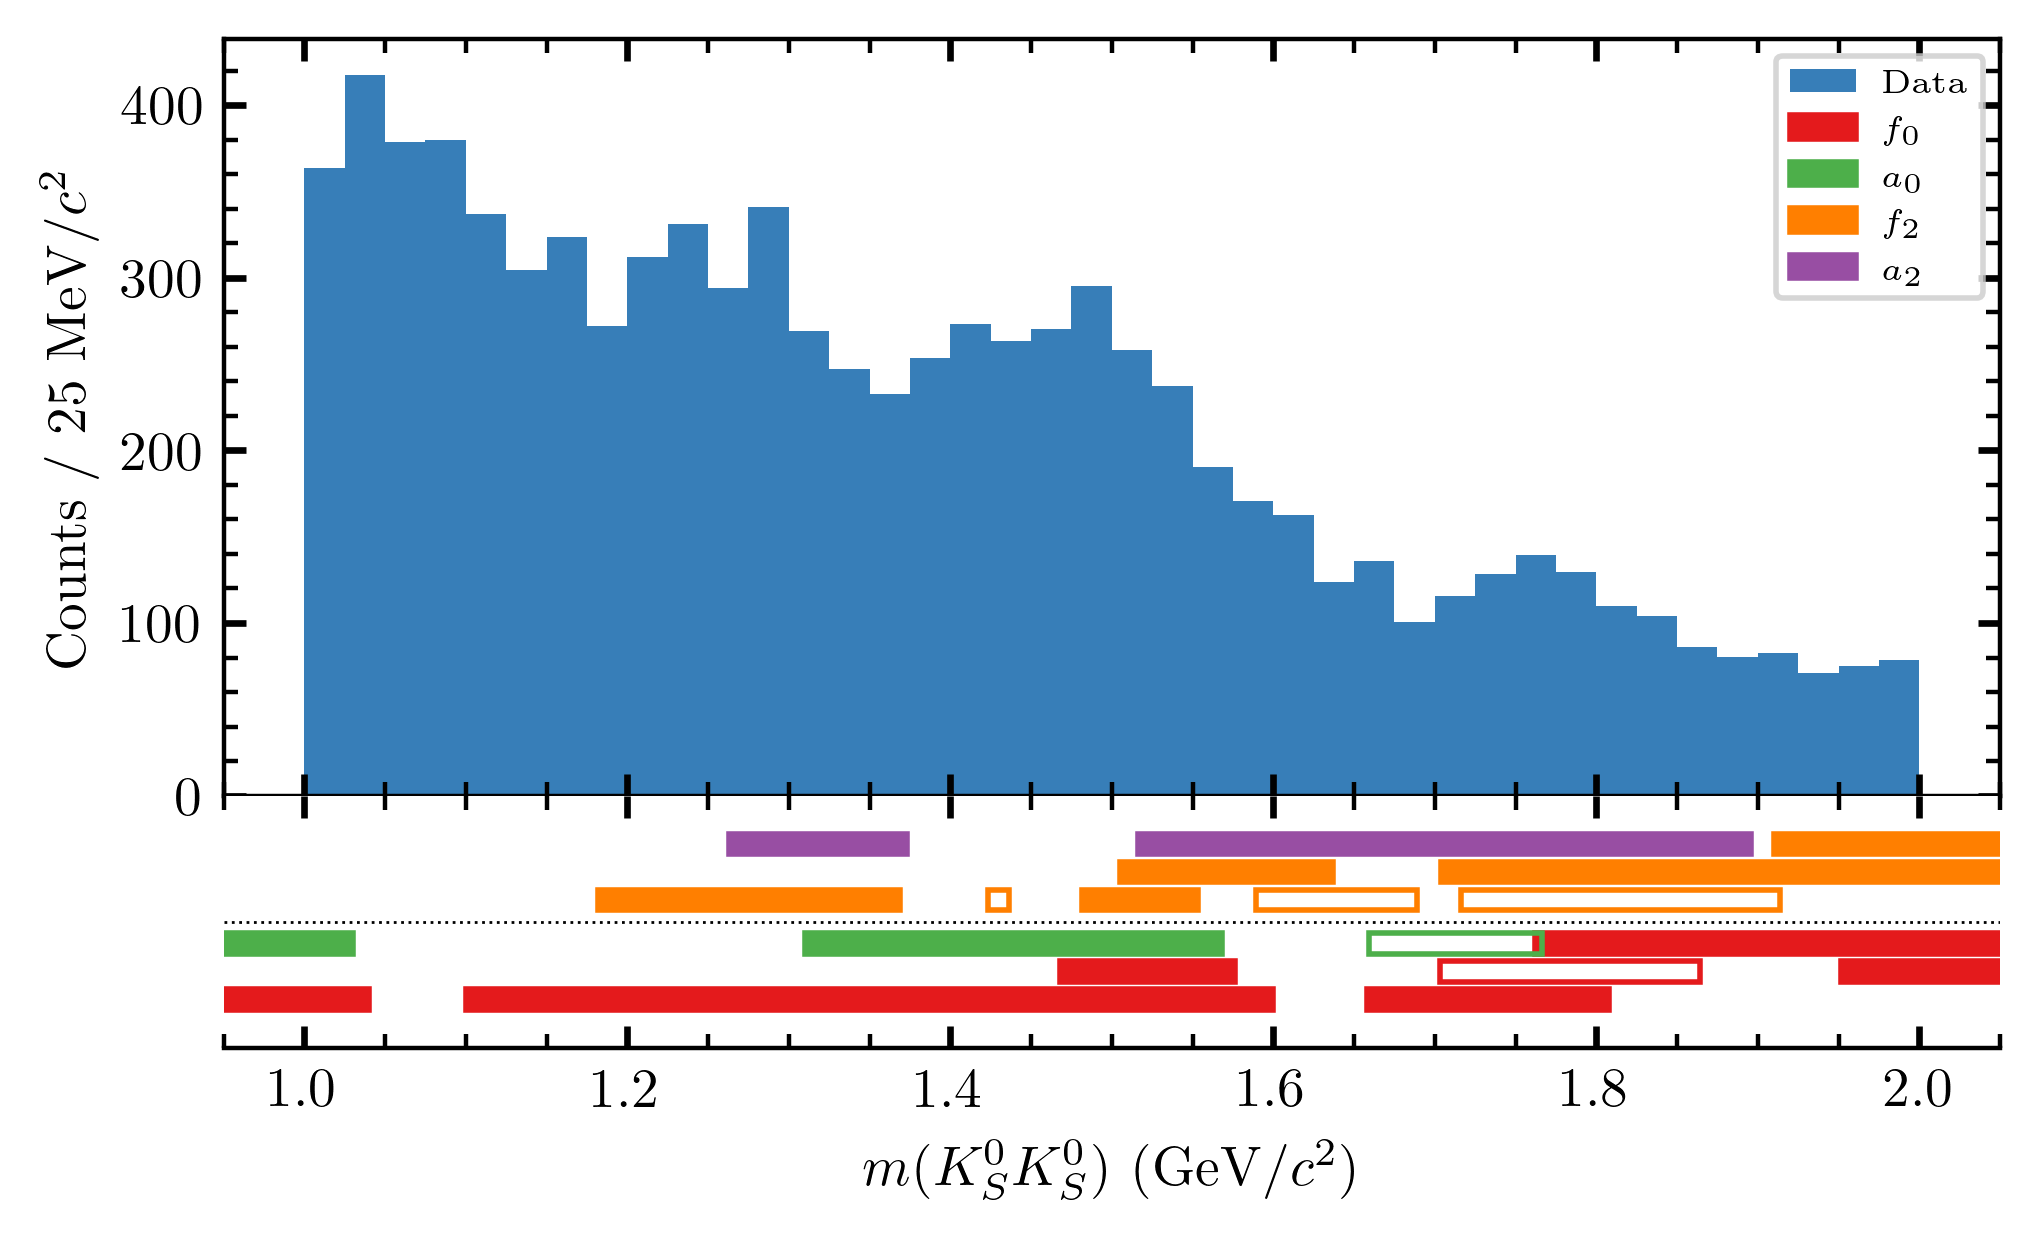
\includegraphics[width=0.8\textwidth]{figures/mass_pdg_data_accpol_chisqdof_3.4_splot_D_1s_2b.png}
  \end{center}
  \caption{The invariant mass of $K_S^0K_S^0$ plotted alongside expected resonances from the PDG~\cite{Zyla2020}. Each rectangle represents a resonance, and the position and width of the rectangle corresponds to the mass and width of the resonance in the PDG. Unfilled rectangles represent particles which have not been firmly established by experiment. There is no meaning to the vertical positioning of the rectangles other than the grouping of spin-$0$ and spin-$2$ resonances on either side of the dotted line. {\color{red}TODO: indicate the centers or the edges that are cut off}}\label{fig:mass-with-pdg}
\end{figure}

To get an idea of what we might expect to see in these fits, we can examine the distribution of $\cos\theta_\text{HX}$ with respect to the invariant mass in \Cref{fig:costheta-vs-mass}. If we think of binning in mass as akin to slicing this figure into vertical strips, then we can compare each bin to the expected shape of the waves in \Cref{fig:spherical-harmonics}. In this way, we might expect the region in $\qtyrange{1.2}{1.6}{\giga\electronvolt}$ to predominantly correspond to the $m=\pm 2$ projection (along with an $S$-wave), since the distribution peaks at the center and falls off at the extreme forward and backward angles. A $D_0$ wave would also peak in the center, but we would expect it to grow rapidly in the forward and backward directions. Similarly, a $D_1$ wave would decay in the forward and backward directions, but would also show a dip in the center.

\begin{figure}
  \begin{center}
    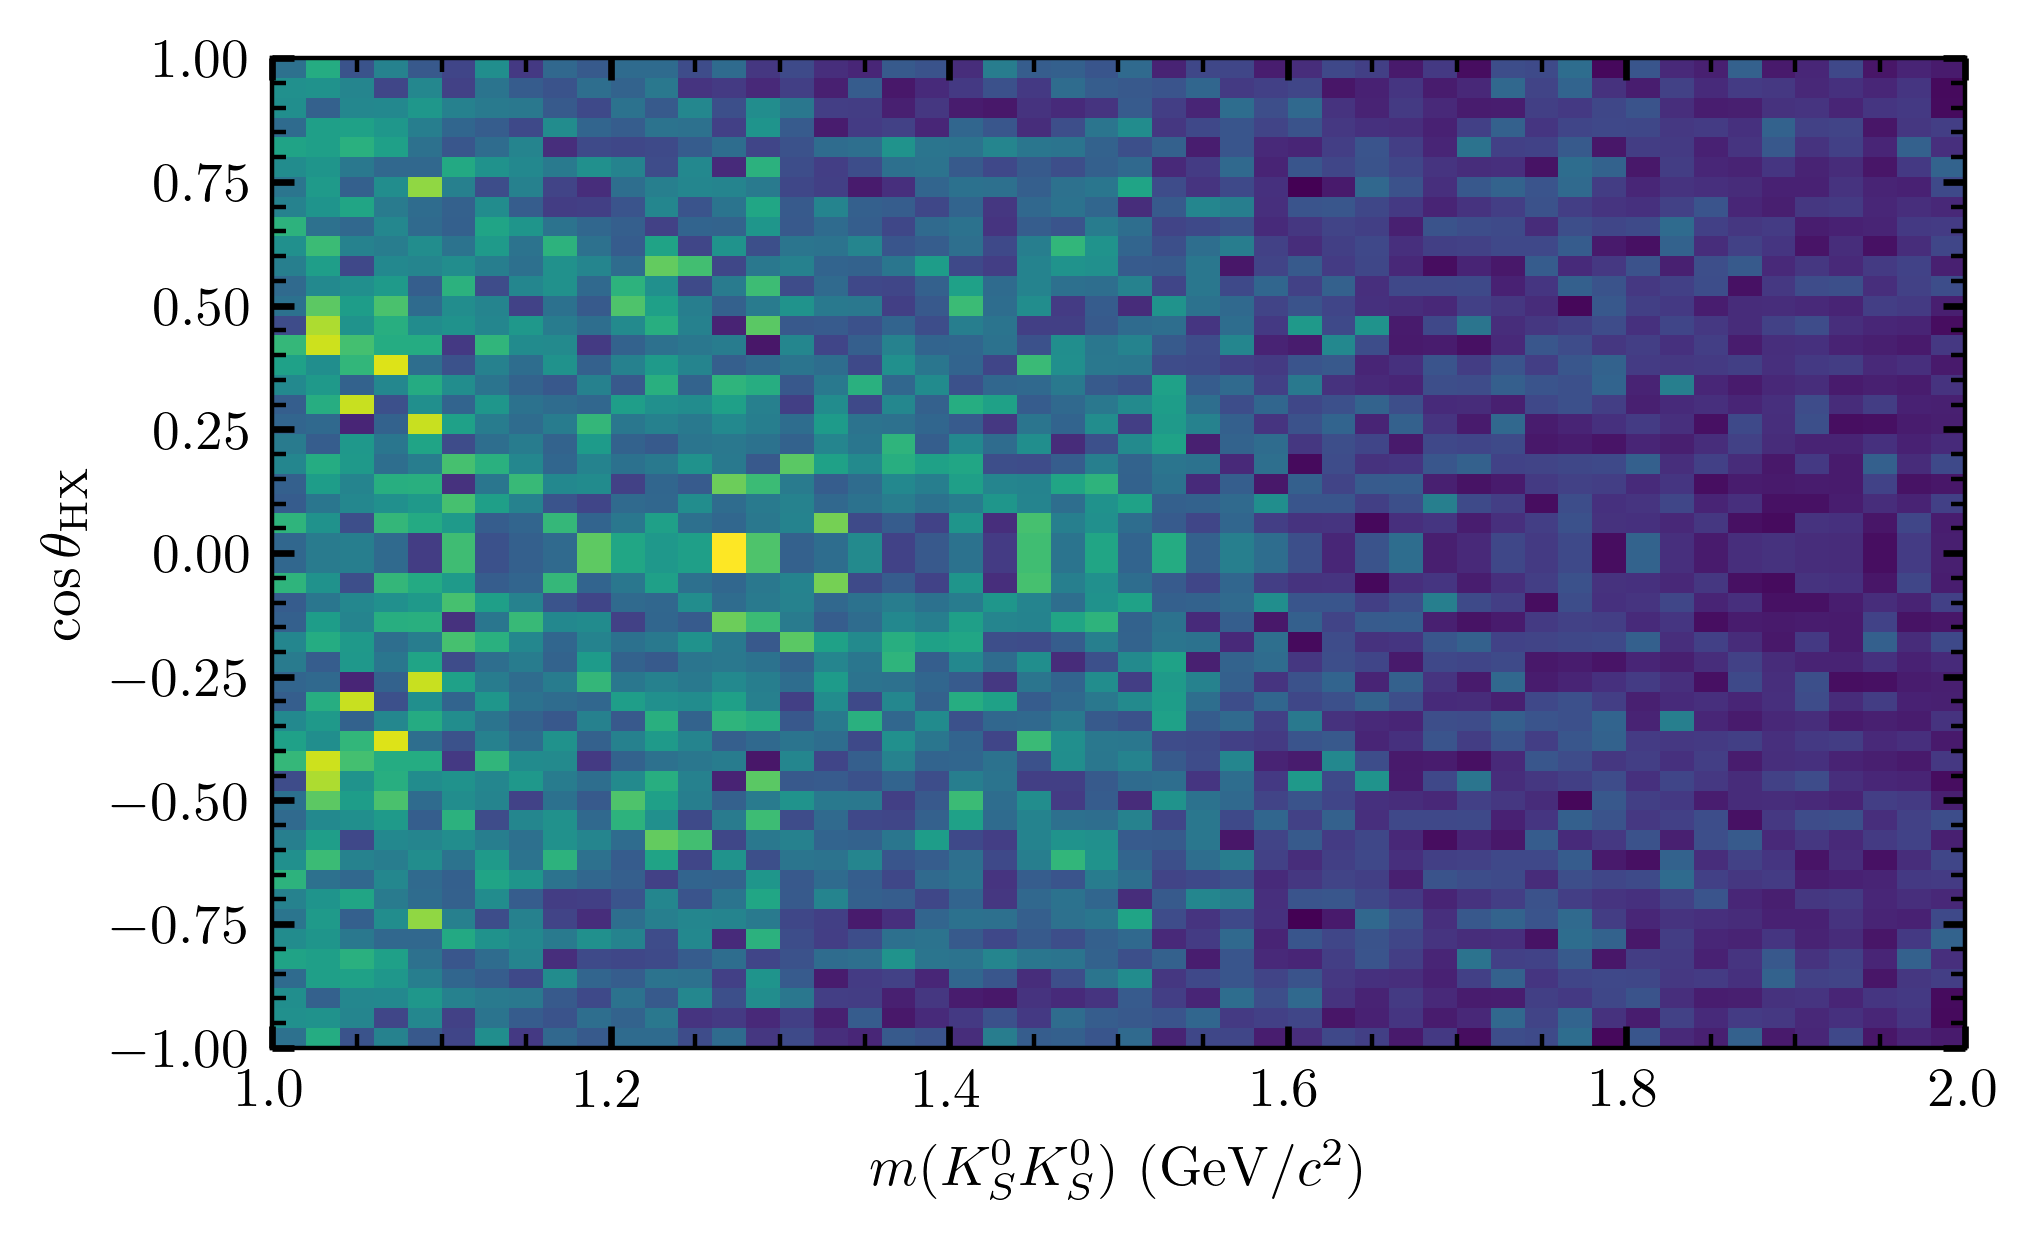
\includegraphics[width=0.95\textwidth]{figures/costheta_data_accpol_chisqdof_3.4_splot_D_1s_2b.png}
  \end{center}
  \caption{A plot of the distribution of $\cos\theta_\text{HX}$ with respect to the invariant mass after all analysis selections and weightings have been applied.}\label{fig:costheta-vs-mass}
\end{figure}

\begin{figure}
  \begin{center}
    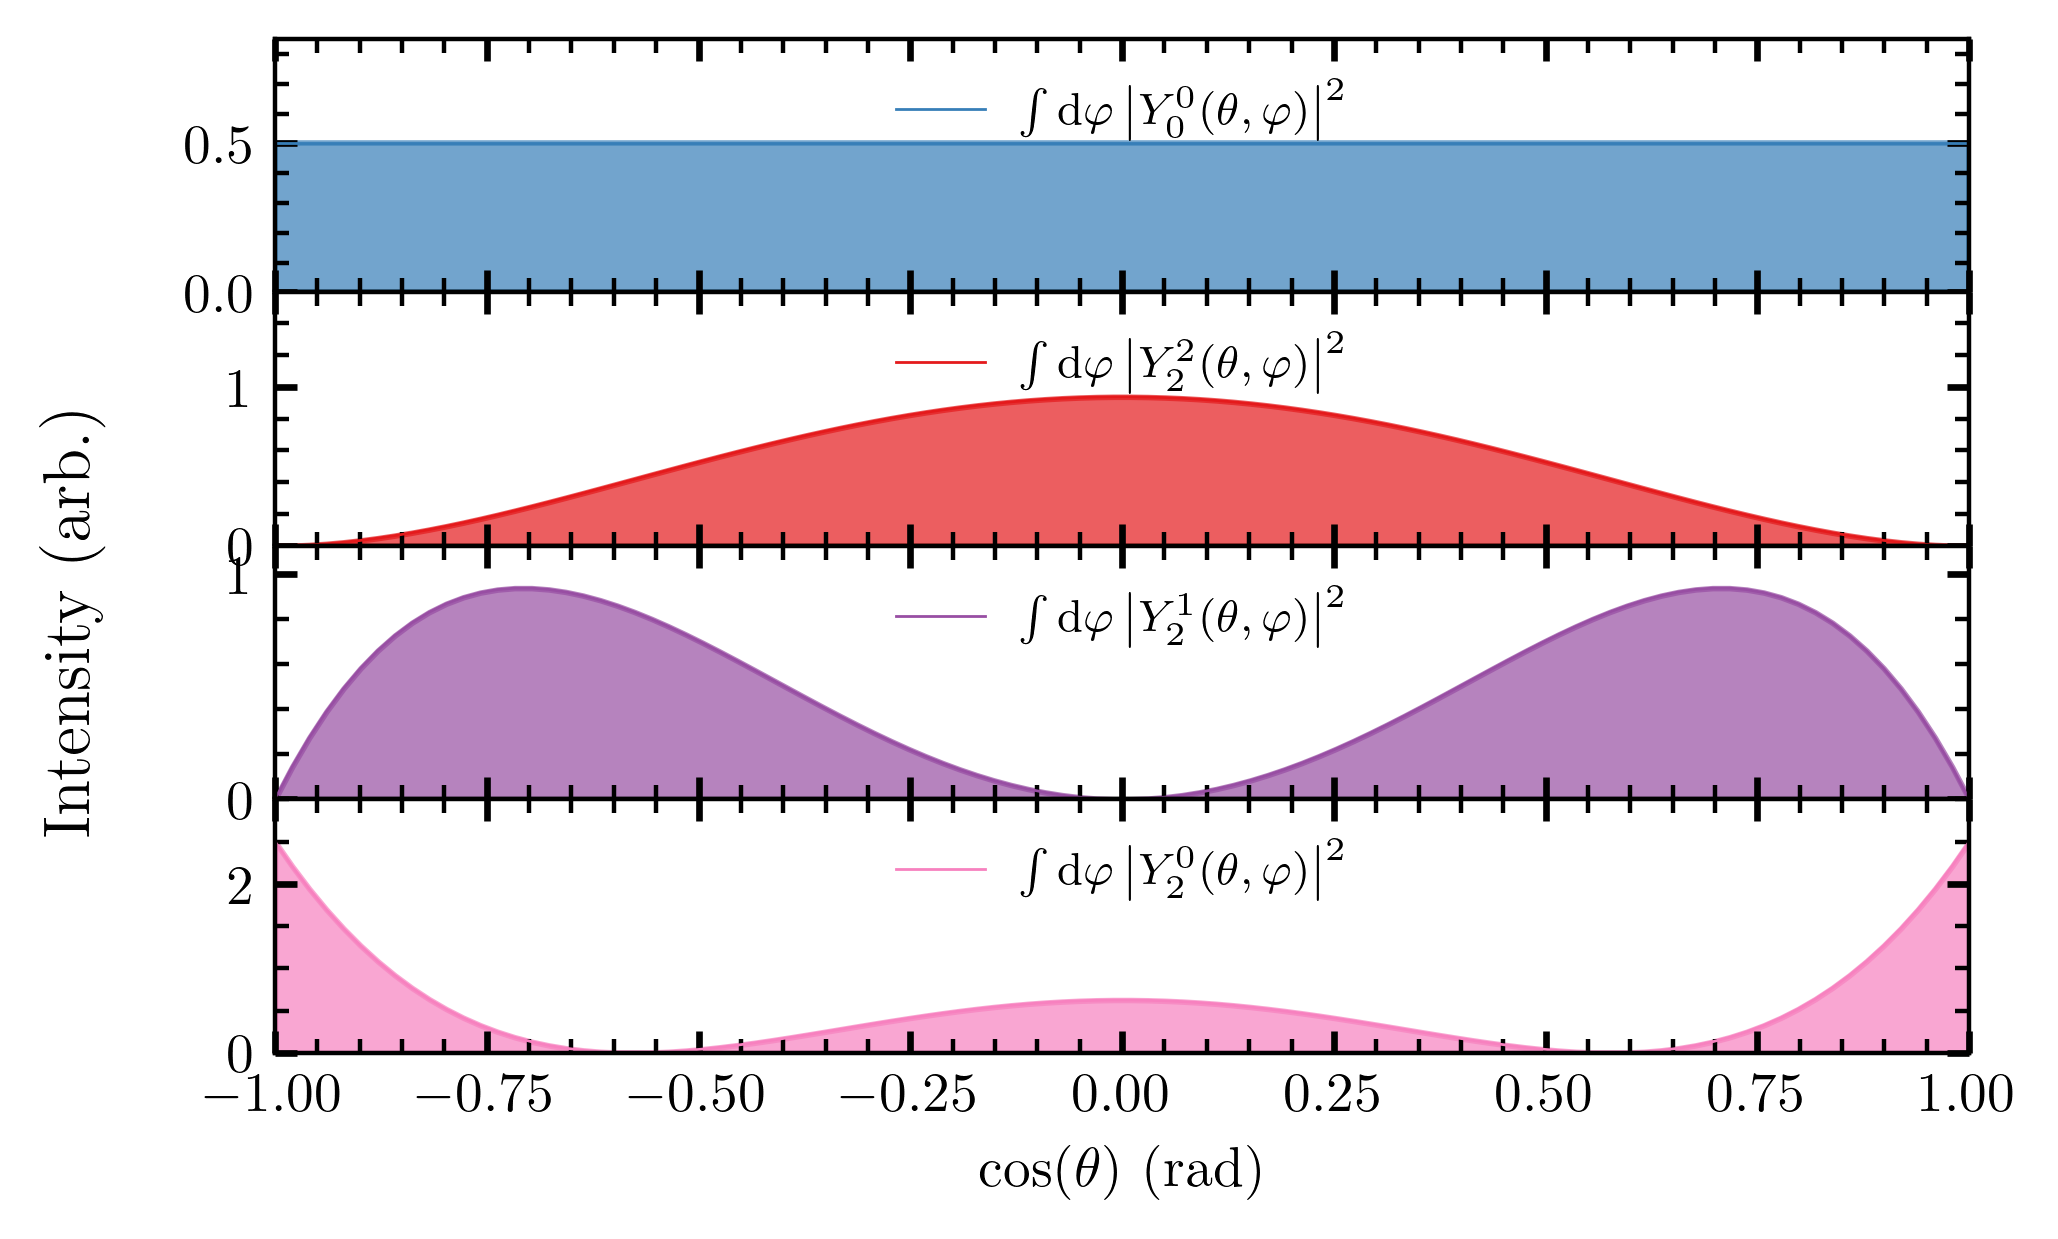
\includegraphics[width=0.8\textwidth]{figures/spherical_harmonics.png}
  \end{center}
  \caption{The expected normalized projections of several spherical harmonics which may be present in the data, integrated over $\varphi$.}\label{fig:spherical-harmonics}
\end{figure}

Examining the angular distribution is a good first step, but it is more prudent to perform fits with each wave to see how well they represent the data. The fitting procedure begins with dividing the data into bins of invariant $K_S^0K_S^0$ mass. In each bin, we fit \Cref{eq:generalized-polarized-intensity} via the method described in \Cref{sec:fitting-methods}. We let each $\hat{T}_{M;\eta}^{J(\epsilon)}$ be a free complex parameter in each bin\footnote{We ignore the sum over the nucleon spin-flip index, $\eta$, since it is not measurable by this experiment.}. The $S$-wave amplitude is just given by a real scalar parameter, since the total form of the intensity is invariant up to a total phase in each coherent sum\footnote{Similarly, when negative reflectivity waves are included, the $S_0^{(-)}$ wave will also be purely real.}. Each bin in mass is fit independently, and the results can be seen in \Cref{fig:binned-fit-chisqdof-3.4-Sp-D0p,fig:binned-fit-chisqdof-3.4-Sp-D1p,fig:binned-fit-chisqdof-3.4-Sp-D2p}. It appears our visual examination of \Cref{fig:costheta-vs-mass} was indeed descriptive, since only the $D_2^{(+)}$ wave has a significant projection onto the data.

Additionally, the binned fit for this wave exhibits two clear peaks, one at around $\SI{1.3}{\giga\electronvolt}$ and one around $\SI{1.5}{\giga\electronvolt}$. We expect these to correspond to the well-established $f_2(1270)$, $a_2(1320)$, and $f_2'(1525)$ resonances (see \Cref{tab:pdg-resonances}). 


\begin{table}
  \begin{center}
    \begin{tabular}{ccc}\toprule
      Resonance & Mass ($\si{\mega\electronvolt}/c^2$) & Width ($\si{\mega\electronvolt}/c^2$)\\\midrule
      $f_0(500)^{\ast}$ & $400$\textendash$800$ & $100$\textendash$800$ \\
      $f_0(980)$ & $990\pm 20$ & $10$\textendash$100$ \\
      $a_0(980)$ & $980\pm 20$ & $50$\textendash$100$ \\
      $f_2(1270)$ & $1275.4 \pm 0.8$ & $186.6^{+2.8}_{-2.2}$ \\
      $a_2(1320)$ & $1318.2 \pm 0.6$ & $109.8\pm 2.4$ \\
      $f_0(1370)$ & $1200$\textendash$1500$ & $200$\textendash$500$ \\
      $f_2(1430)^{\ast\dagger}$ & $\approx 1430$ & $\approx 13$\textendash$43$ \\
      $a_0(1450)$ & $1439\pm 34$ & $258\pm 14$ \\
      $f_0(1500)$ & $1522\pm 25$ & $108\pm 33$ \\
      $f_2'(1525)$ & $1517.3\pm 2.4$ & $72^{+7}_{-6}$ \\
      $f_2(1640)^{\ast\dagger}$ & $1639\pm 6$ & $100^{+60}_{-40}$ \\
      $a_2(1700)$ & $1706\pm 14$ & $380^{+60}_{-50}$ \\
      $a_0(1710)^{\ast\dagger}$ & $1713\pm 19$ & $107\pm 15$ \\
      $f_0(1710)$ & $1733^{+8}_{-7}$ & $150^{+12}_{-10}$ \\
      $f_0(1770)^{\ast\dagger}$ & $1784^{+16}_{-14}$ & $161\pm 21$ \\
      $f_2(1810)^{\dagger}$ & $1815\pm 12$ & $197\pm 22$ \\
      $f_2(1910)^{\ast\dagger}$ & $1941\pm 182$ & $120\pm 40$ \\
      $a_0(1950)^{\ast\dagger}$ & $1931\pm 26$ & $270\pm 40$ \\
      $f_2(1950)$ & $1936\pm 12$ & $464\pm 24$ \\
      $f_2(2010)^{\ast}$ & $2010^{+60}_{-80}$ & $200\pm 60$ \\
      $f_0(2020)^{\ast}$ & $1982^{+54.1}_{-3.0}$ & $440\pm 50$ \\
      $f_0(2100)^{\ast\dagger}$ & $2095^{+17}_{-19}$ & $287^{+32}_{-24}$ \\
      $f_2(2150)^{\ast\dagger}$ & $2157\pm 12$ & $152\pm 30$ \\
      $f_0(2200)^{\ast\dagger}$ & $2187\pm 14$ & $210\pm 40$ \\\bottomrule
    \end{tabular}
    \caption{Resonances along with their approximate masses and widths from the PDG~\cite{Zyla2020} with quantum numbers compatible with the $K_S^0K_S^0$ channel. Resonances marked with an asterisk ($\ast$) are not included in the $K$-matrix model for the mass-dependent fits. Resonances marked with a dagger ($\dagger$) are not well-established according to the PDG.}\label{tab:pdg-resonances}
  \end{center}
\end{table}


\begin{figure}
  \begin{center}
    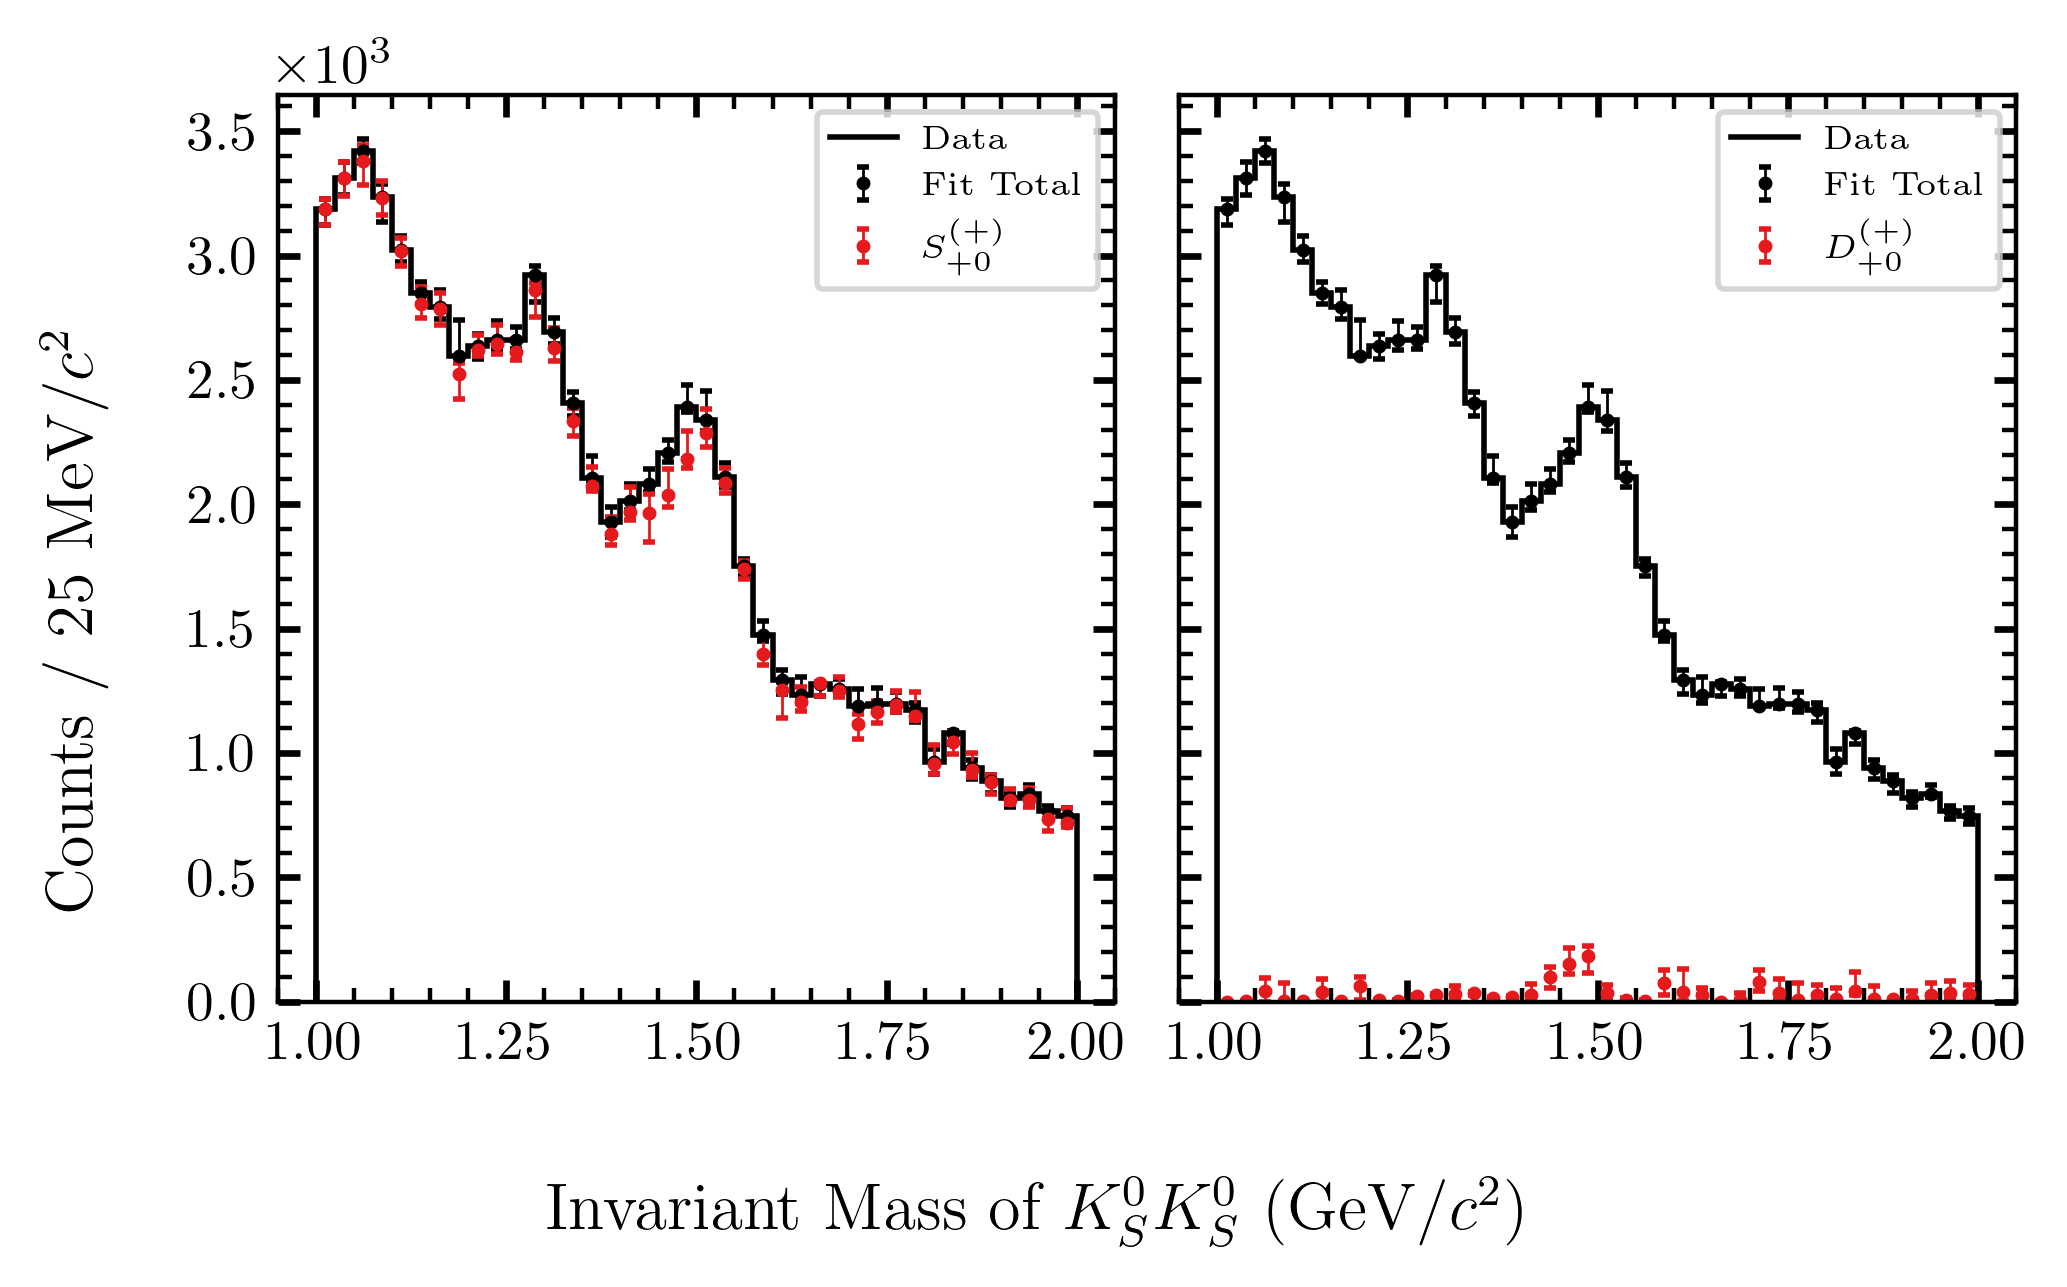
\includegraphics[width=0.8\textwidth]{figures/binned_fit_chisqdof_3.4_splot_D_1s_2b_phase_factor_waves487_uncertainty_bootstrap-CI-BC.png}
  \end{center}
  \caption{Binned fit of $S_{0}^{(+)}$ and $D_{0}^{(+)}$ waves. Bars on each fit point correspond to $68\%$ bias-corrected confidence intervals over $ 30 $ bootstrap iterations.}\label{fig:binned-fit-chisqdof-3.4-Sp-D0p}
\end{figure}
\begin{figure}
  \begin{center}
    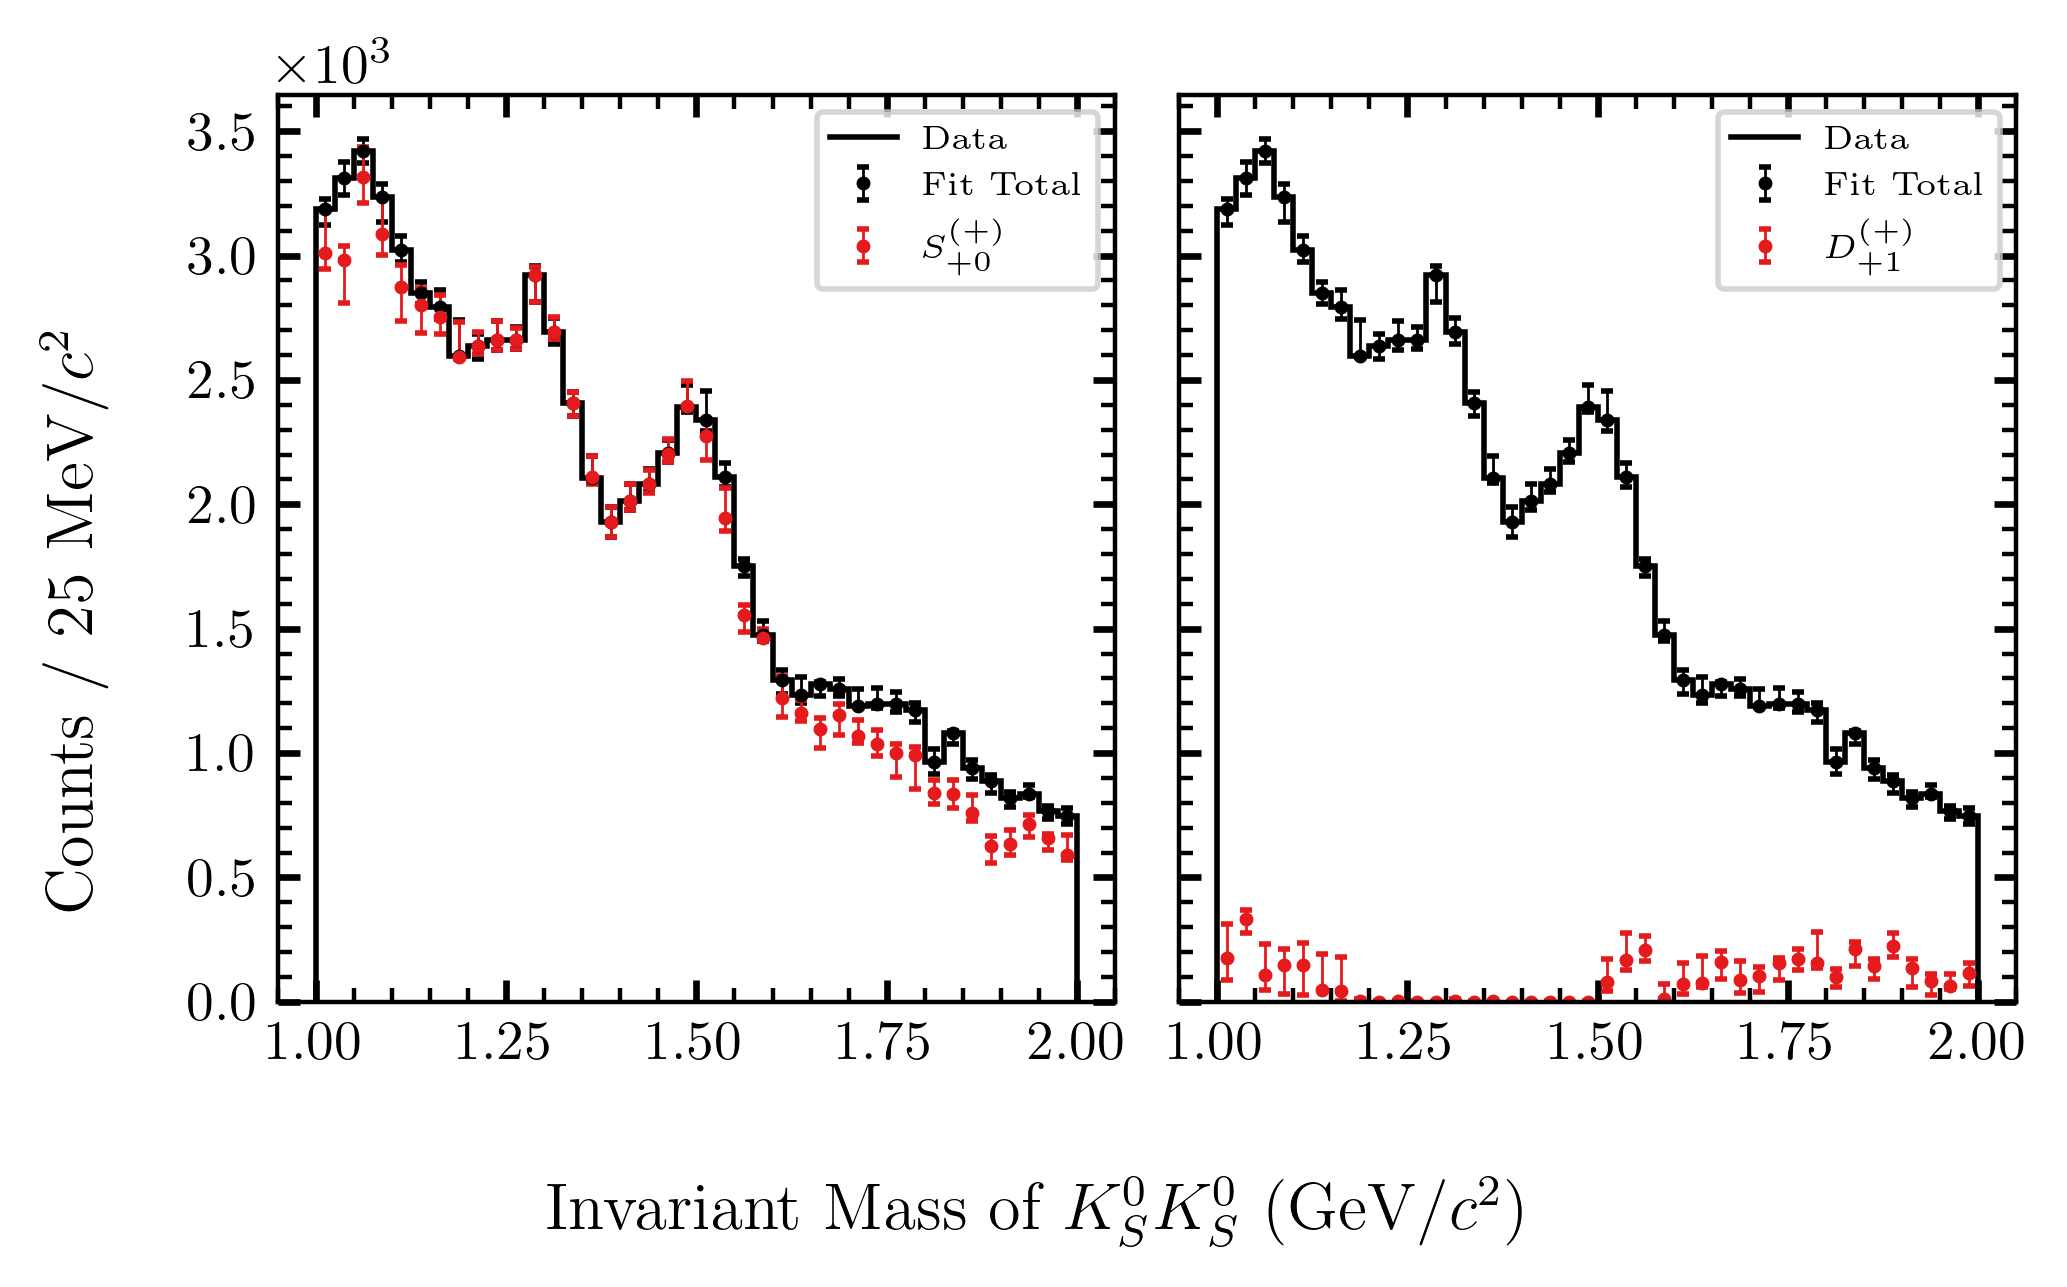
\includegraphics[width=0.8\textwidth]{figures/binned_fit_chisqdof_3.4_splot_D_1s_2b_phase_factor_waves489_uncertainty_bootstrap-CI-BC.png}
  \end{center}
  \caption{Binned fit of $S_{0}^{(+)}$ and $D_{+1}^{(+)}$ waves. Bars on each fit point correspond to $68\%$ bias-corrected confidence intervals over $ 30 $ bootstrap iterations.}\label{fig:binned-fit-chisqdof-3.4-Sp-D1p}
\end{figure}
\begin{figure}
  \begin{center}
    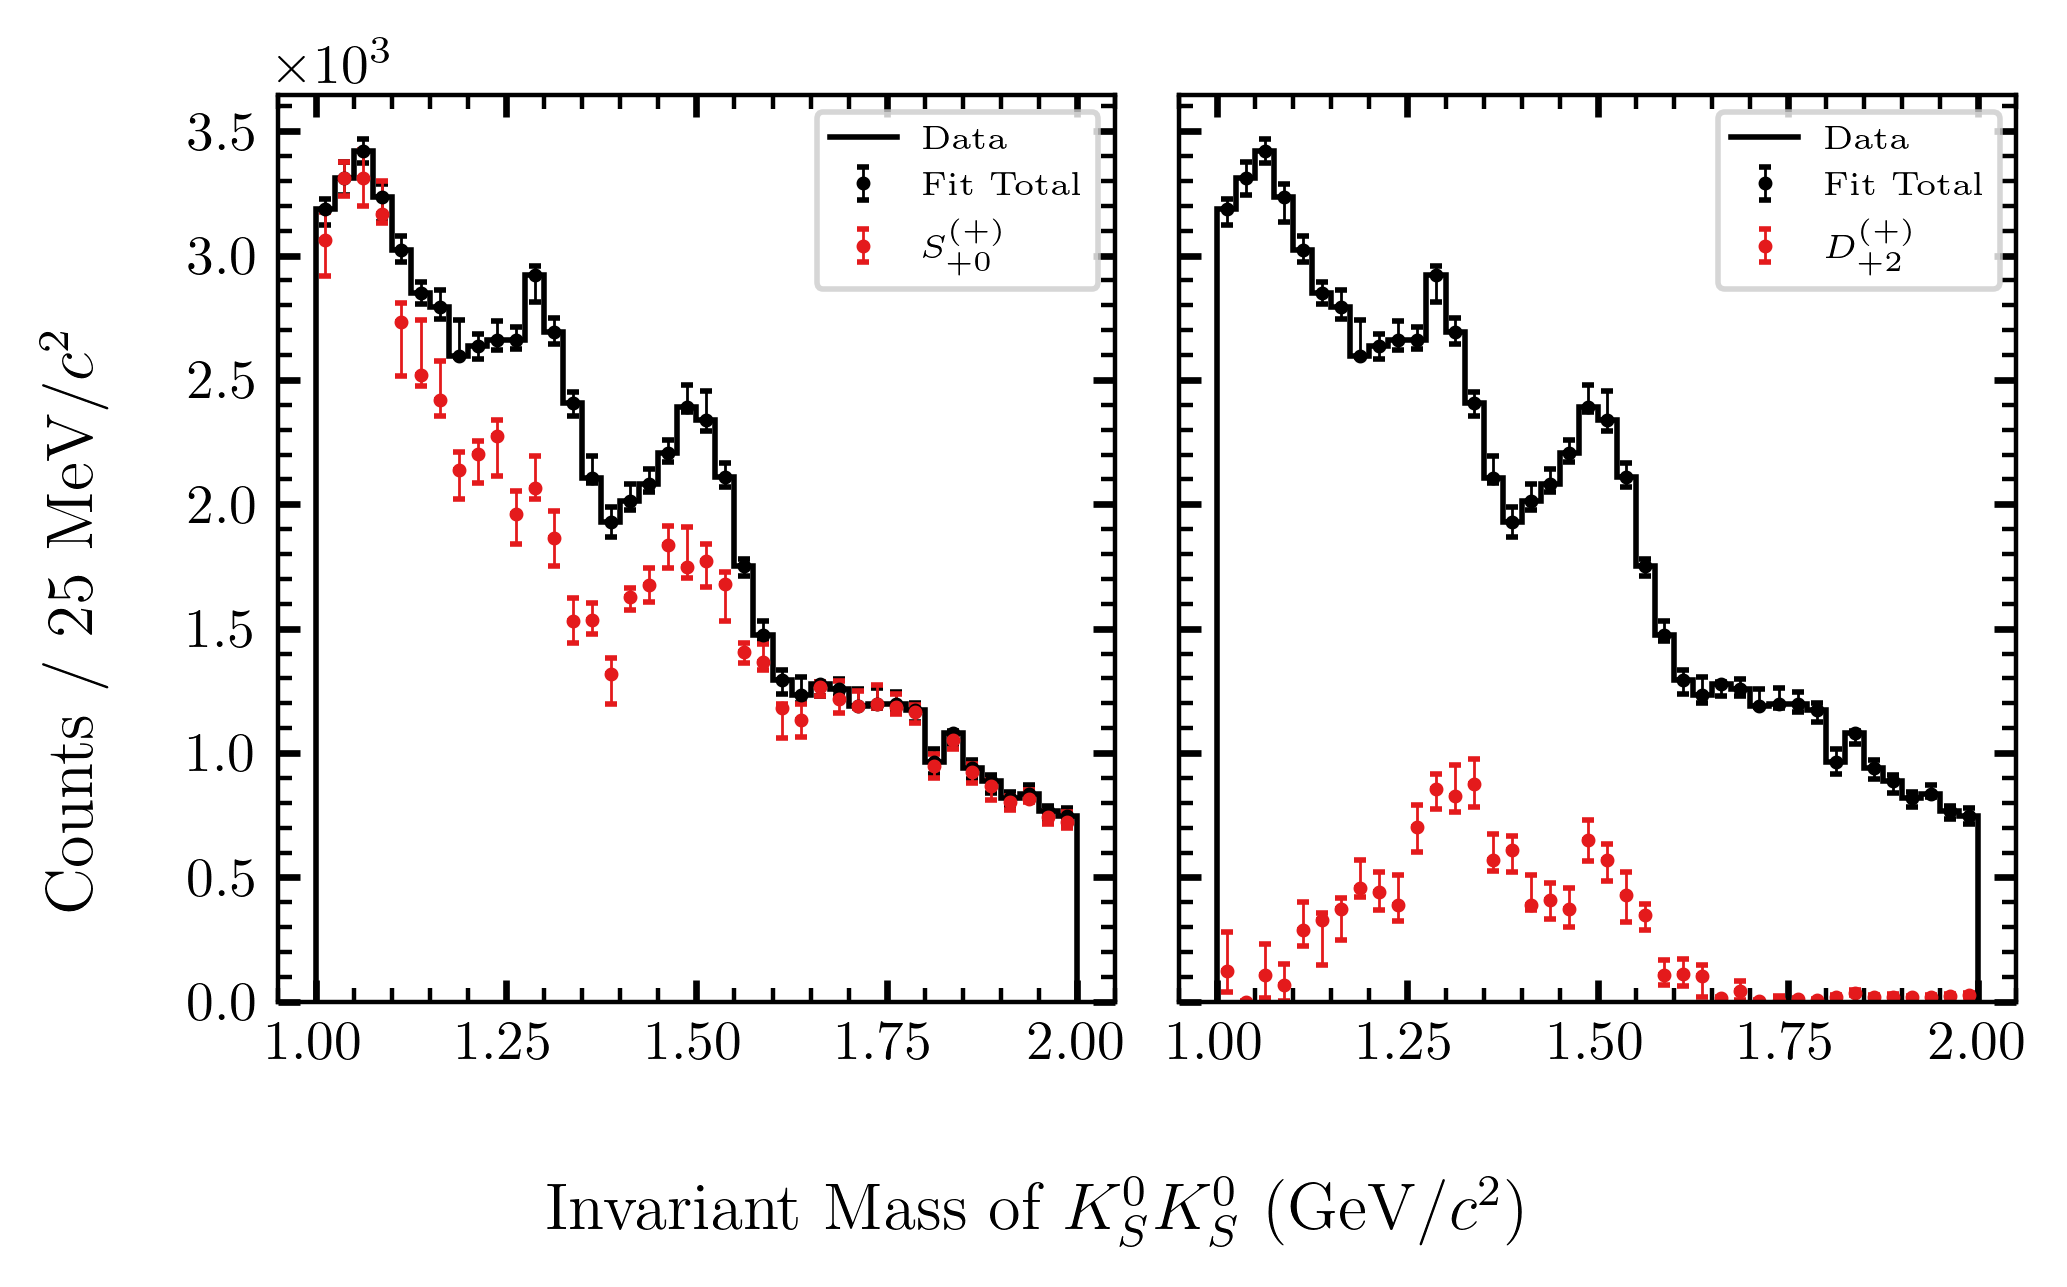
\includegraphics[width=0.8\textwidth]{figures/binned_fit_chisqdof_3.4_splot_D_1s_2b_phase_factor_waves491_uncertainty_bootstrap-CI-BC.png}
  \end{center}
  \caption{Binned fit of $S_{0}^{(+)}$ and $D_{+2}^{(+)}$ waves. Bars on each fit point correspond to $68\%$ bias-corrected confidence intervals over $ 30 $ bootstrap iterations.}\label{fig:binned-fit-chisqdof-3.4-Sp-D2p}
\end{figure}

We can also sum the negative log-likelihoods from each bin in each fit to get a total likelihood for each fit. Since each fit has the same number of free parameters, we can directly compare the negative log-likelihoods, which are {\color{red}TODO} $?$, $?$, and $?$ for the fits involving $D_0^{(+)}$, $D_1^{(+)}$, and $D_2^{(+)}$ waves respectively. We can conclude that the $D_2^{(+)}$ wave model is the most likely to describe the data, since it has the lowest negative log-likelihood.

While we could imagine that interference effects between waves could cause the non-$D_2$ waves to have a non-negligible projection onto the data, we must focus on the minimal set of waves required to fit the data. The next wave we will add to this model will be a negative-reflectivity $S$-wave. In the model, waves only interfere with waves of the same reflectivity, so we should expect the $D$-wave to be largely unaffected by this additional wave. However, since the existing $S_0^{(+)}$ wave will be reduced non-trivially in each bin, it is possible that the $D_2^{(+)}$ wave projection may change slightly in regions where the $S_0^{(-)}$ component is large. We can see the result of this fit in \Cref{fig:binned-fit-chisqdof-3.4-Spn-D2p}. The notable difference between this fit and the previous fit without the $S_0^{(-)}$ wave is that the $S_0^{(+)}$ wave no longer has the large bump around $\SI{1.5}{\giga\electronvolt}$ which was likely due to a combination of the $a_0(1450)$ and $f_0(1500)$. Instead, we still see a slight enhancement in the positive-reflectivity $S$-wave, but there is a much more noticeable peak in the negative-reflectivity $S$-wave right at $\SI{1.5}{\giga\electronvolt}$. Referencing \Cref{tab:pdg-resonances}, there is only one narrow spin-$0$ resonance around this mass, viz. the $f_0(1500)$. Since positive/negative reflectivity corresponds to natural/unnatural parity exchange in this $t$-channel interaction, the fit may suggest that $f_0(1500)$ production is mostly produced by some unnatural parity exchange process, or at least some percentage of the resonant production follows a different production process.

{\color{red}TODO: CLAS comparison}

{\color{red}TODO: Add $D_2^{(-)}$ wave?}

\begin{figure}
  \begin{center}
    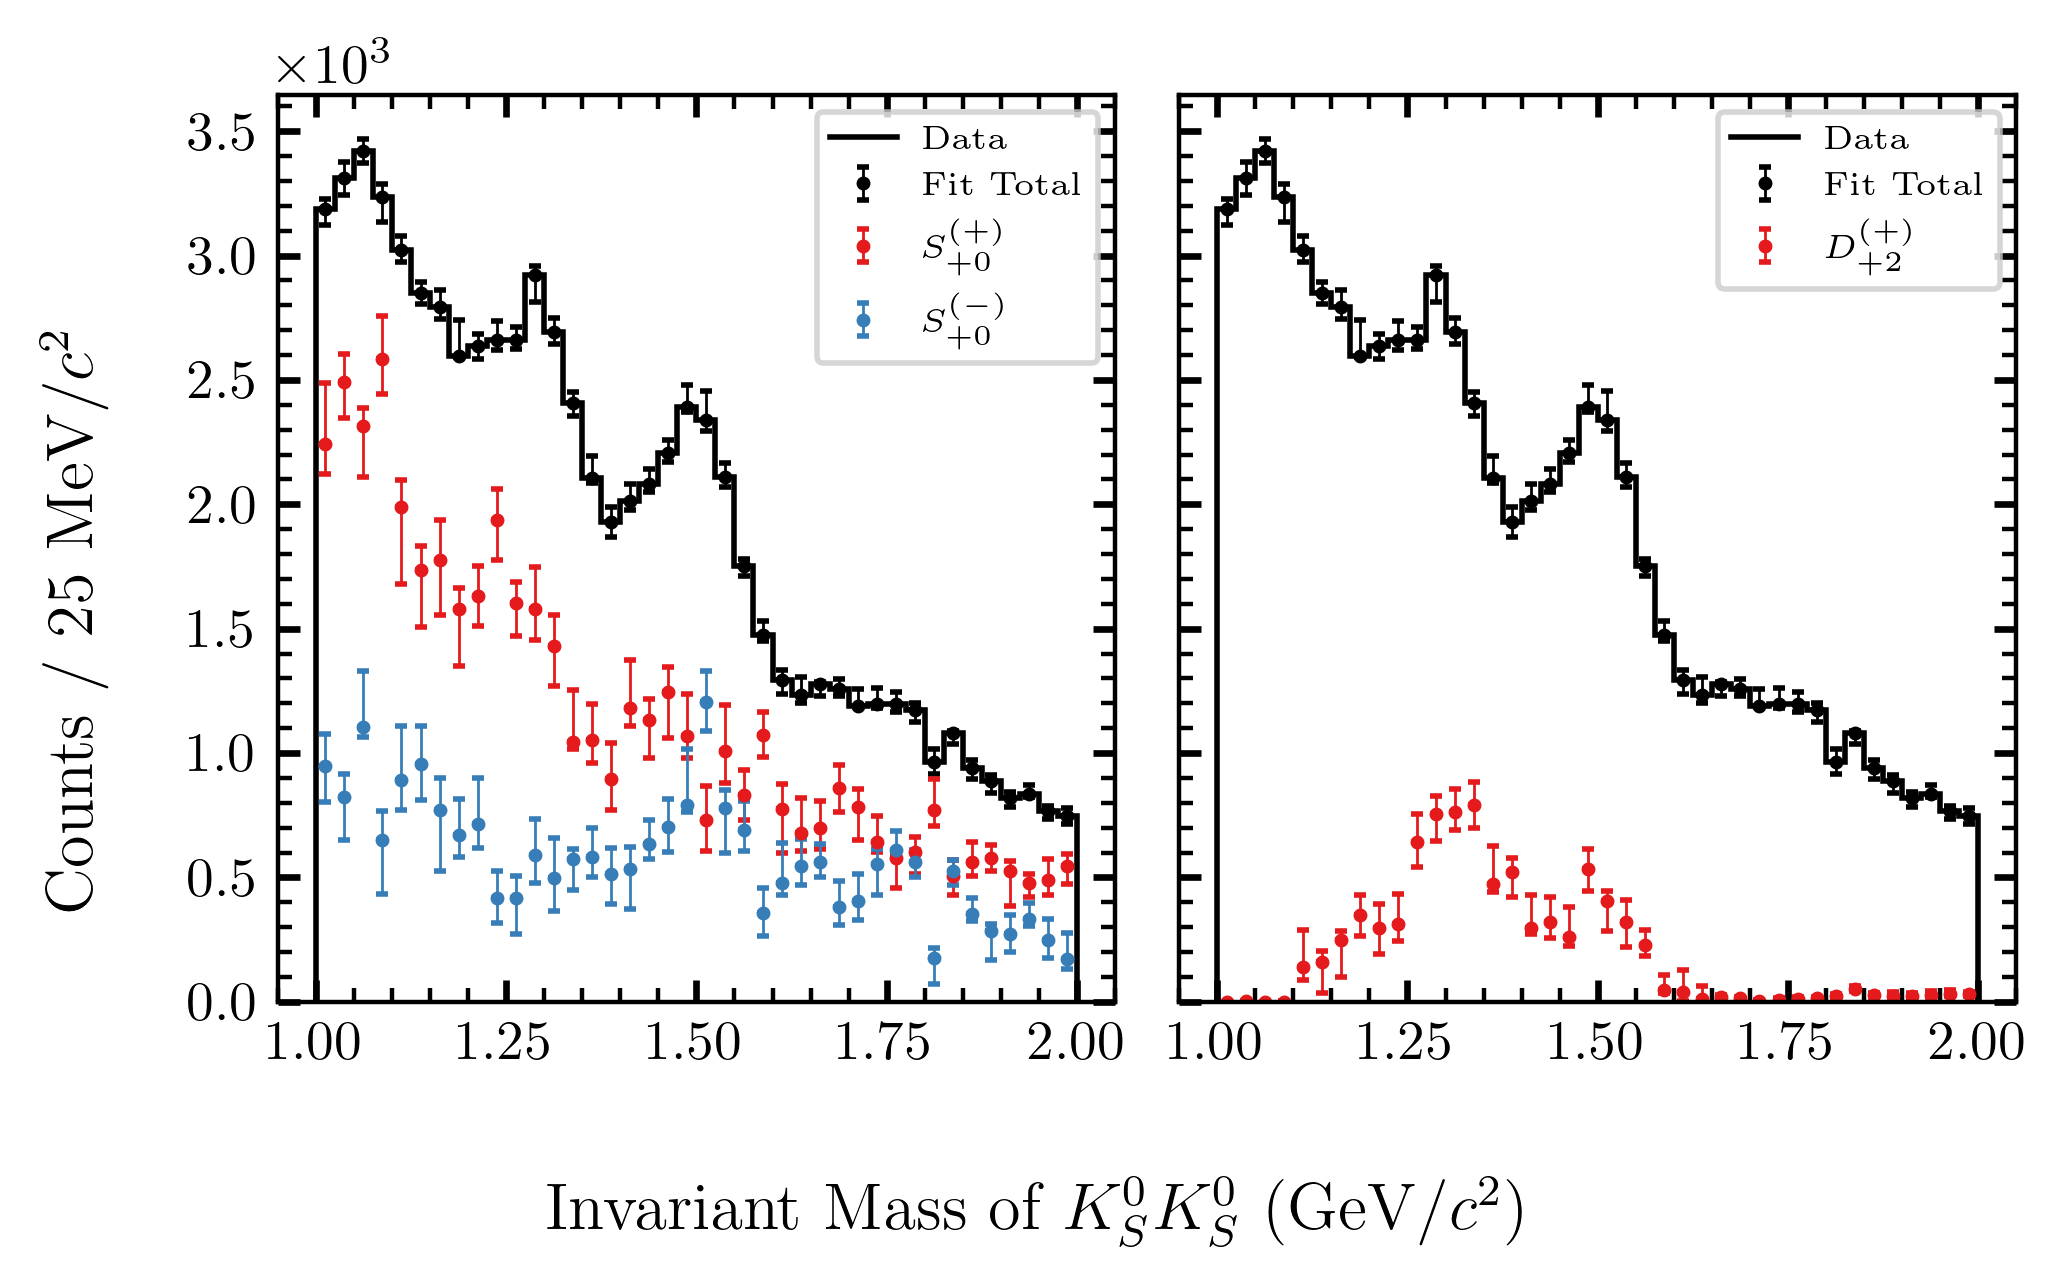
\includegraphics[width=0.8\textwidth]{figures/binned_fit_chisqdof_3.4_splot_D_1s_2b_phase_factor_waves29099_uncertainty_bootstrap-CI-BC.png}
  \end{center}
  \caption{Binned fit of $S_{0}^{(+)}$, $S_{0}^{(-)}$, and $D_{+2}^{(+)}$ waves. Bars on each fit point correspond to $68\%$ bias-corrected confidence intervals over $ 30 $ bootstrap iterations.}\label{fig:binned-fit-chisqdof-3.4-Spn-D2p}
\end{figure}



\section{Mass-Dependent Fits}\label{sec:mass-dependent-fits}

We now turn our attention to the $K$-matrix formalism discussed in \Cref{sec:k-matrix}. We could restrict the $K$-matrix to a single channel and fit both the production couplings ($\beta_\alpha$) and decay couplings ($g_{i\alpha}$) along with the mass poles ($m_\alpha$), and this would ostensibly result in the same number of free parameters as would Breit-Wigner peaks for each resonance. However, the key point of the $K$-matrix is that it also describes the effect on resonances when a threshold energy is crossed and a channel is opened up, and this cannot be similarly captured with a single-channel approach. In the case of $K_S^0K_S^0$, the threshold production of the $f_0(980)$ and $a_0(980)$ is problematic for several reasons. First, both of these resonances have mass poles just smaller than the threshold for producing two $K_S^0$s, so the lineshape may be dependent on the coupling to other channels. Second, these particles differ only in isospin, which is not observable in the $K_S^0K_S^0$ channel. This makes it very difficult to control for the possible interference effects between the two resonances. Finally, the $\eta'\pi$ channel opens around $\SI{1.093}{\giga\electronvolt}$, and there is evidence that the $a_0(980)$ has a nonzero component in this channel~\cite{Ablikim2017,Chen2020}, and this may also alter the shape of the intensity from these resonances. We can attempt to circumvent the first two issues by using a fixed $K$-matrix. In principle, this is like fixing the masses and widths of a set of Breit-Wigner peaks to known values from literature. However, in practice, it allows us to incorporate some information about the effect of other channels on the intensity. We will use the results of \cite{Albrecht2020} and \cite{Kopf2021} as the basis for the $K$-matrix. This does not help us with the third problem, since the $\eta'\pi$ channel is not included in their fit for the $a_0$ $K$-matrix, but we will assume that their fit accurately covers the most prominent resonances in our region of interest. Using their published values for the decay couplings, mass peaks, and non-resonant background corrections ($\tilde{c}_{nij}$), we construct the $K$-matrix for the $f_0$, $a_0$, $f_2$, and $a_2$ channels accordingly and use these as the parameterization of $\hat{T}_{M;\eta}^{J(\epsilon)}(\vec{\beta};m,s)$ in \Cref{eq:generalized-polarized-intensity}. It should be noted that the values from their fit primarily come from Crystal Barrel data which was taken at a center-of-mass energy of $\sqrt{s} = \SI{2050}{\mega\electronvolt}$. On the other hand, our dataset nominally spans a beam energy range of $\qtyrange{8.0}{8.8}{\giga\electronvolt}$ which corresponds to $\sqrt{s}$ in the range of $\qtyrange{3986}{4170}{\mega\electronvolt}$. \Cref{eq:invariant-k-matrix} includes background terms $\tilde{c}_{nij}$ which may scale differently with energy. However, we cannot leave these parameters floating in the fit, since they depend on data from other decay channels. Therefore, while we will proceed with the use of this fixed $K$-matrix, we should note that the accuracy of this approach is limited\footnote{This was first pointed out to me by Dr. Eric Swanson.}.

We again begin with a fit to only positive-reflectivity waves ($S_0^{(+)}$ and $D_2^{(+)}$), the results of which can be seen in \Cref{fig:unbinned-fit-chisqdof-3.4-Sp-D2p}. While there is some general agreement between the mass-independent fit from the previous section and the mass-dependent fit shown by the shaded histogram, there are also large discrepancies, mostly in the region where the two $D$-wave peaks are located. We will address this shortly, but first we should note that the region around $\SI{1.15}{\giga\electronvolt}$ appears to contain a considerable contribution from the $D_2^{(+)}$ wave, but no spin-$2$ resonances exist in this mass range (or in the $K$-matrix model), so it will always be difficult for a model to account for this region accurately. The exact cause for this enhancement is unclear, but could be due to some background for which we have not yet accounted, and this will be discussed further in \Cref{sec:systematic-studies}.

\begin{figure}
  \begin{center}
    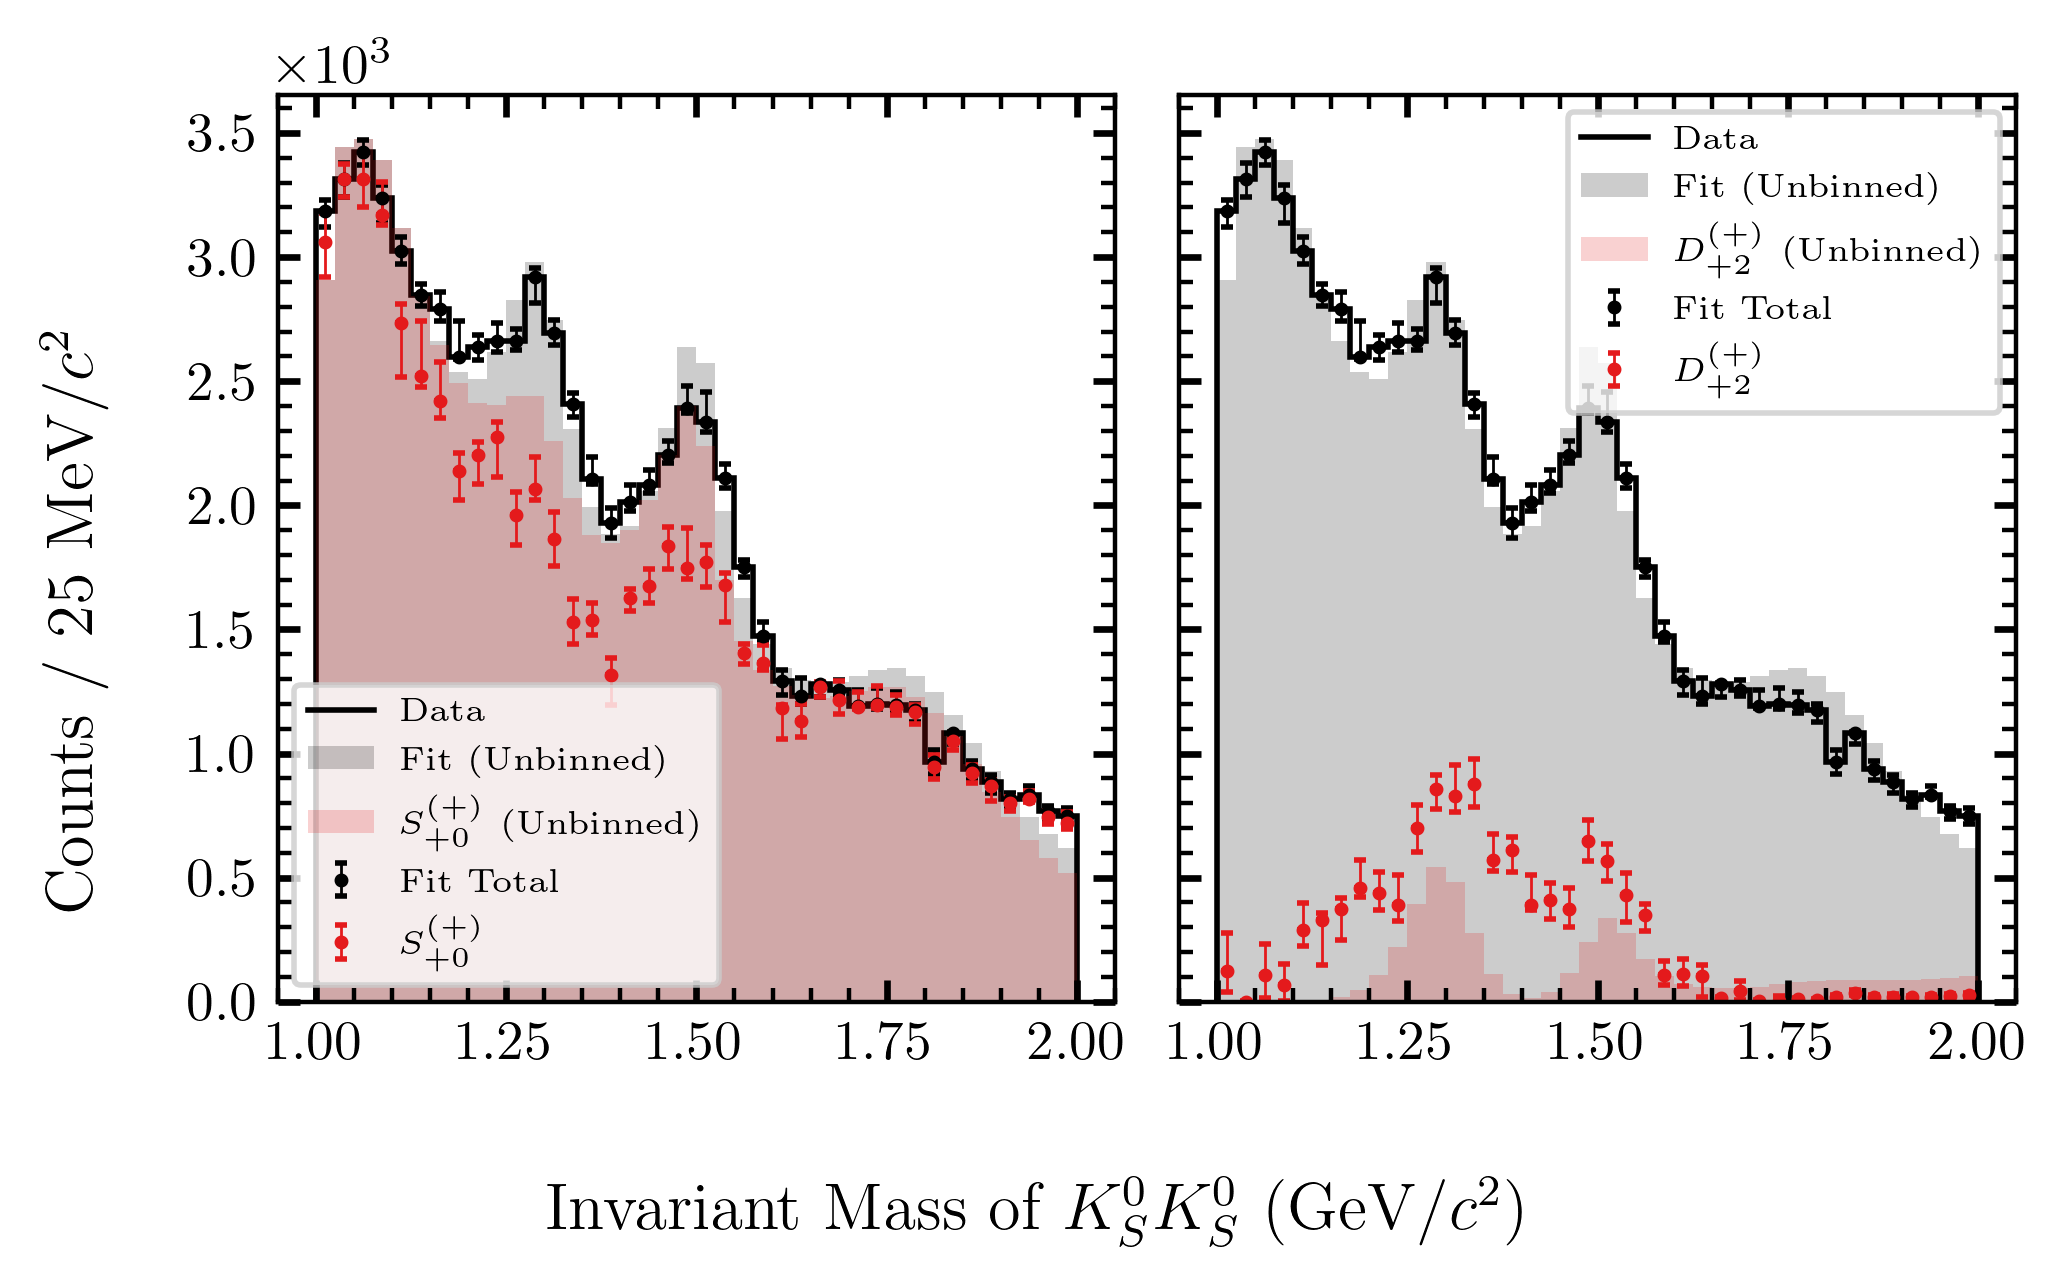
\includegraphics[width=0.8\textwidth]{figures/binned_and_unbinned_fit_chisqdof_3.4_splot_D_1s_2b_phase_factor_waves491_uncertainty_bootstrap-SE.png}
  \end{center}
  \caption{Mass-independent (binned) and mass-dependent (unbinned) fit of $S_{0}^{(+)}$ and $D_{+2}^{(+)}$ waves. Bars on each binned fit point correspond to $68\%$ bias-corrected confidence intervals over $ 30 $ bootstrap iterations.}\label{fig:unbinned-fit-chisqdof-3.4-Sp-D2p}
\end{figure}

As in the previous section, this fit may be extended to a waveset with a negative-reflectivity $S$-wave. The result of this fit can be seen in \Cref{fig:unbinned-fit-chisqdof-3.4-Spn-D2p}. While the spin-$2$ components are still underrepresented, we see generally good agreement between the mass-independent and mass-dependent fits. Some notable discrepancies occur near threshold and around $\SI{1.3}{\giga\electronvolt}$, where the negative-reflectivity $S$-wave is larger than the binned fit would indicate.

Adding additional waves becomes unmanageable, as the number of free parameters grows quickly and the model becomes prone to overfitting. Because there is no ability to distinguish isospin, there are many ways for even the limited parameters we use to converge on similar fits while the underlying projections of each individual resonance may vary greatly. This can unfortunately not be resolved without a coupled channel fit with channels that only contain a single isospin, such as $\pi\pi$, $\eta\pi$, or $\eta'\pi$, and this is beyond the scope of this thesis. However we can improve these results slightly by being more careful about the initialization of the fit, as will be shown in the following section.

\begin{figure}
  \begin{center}
    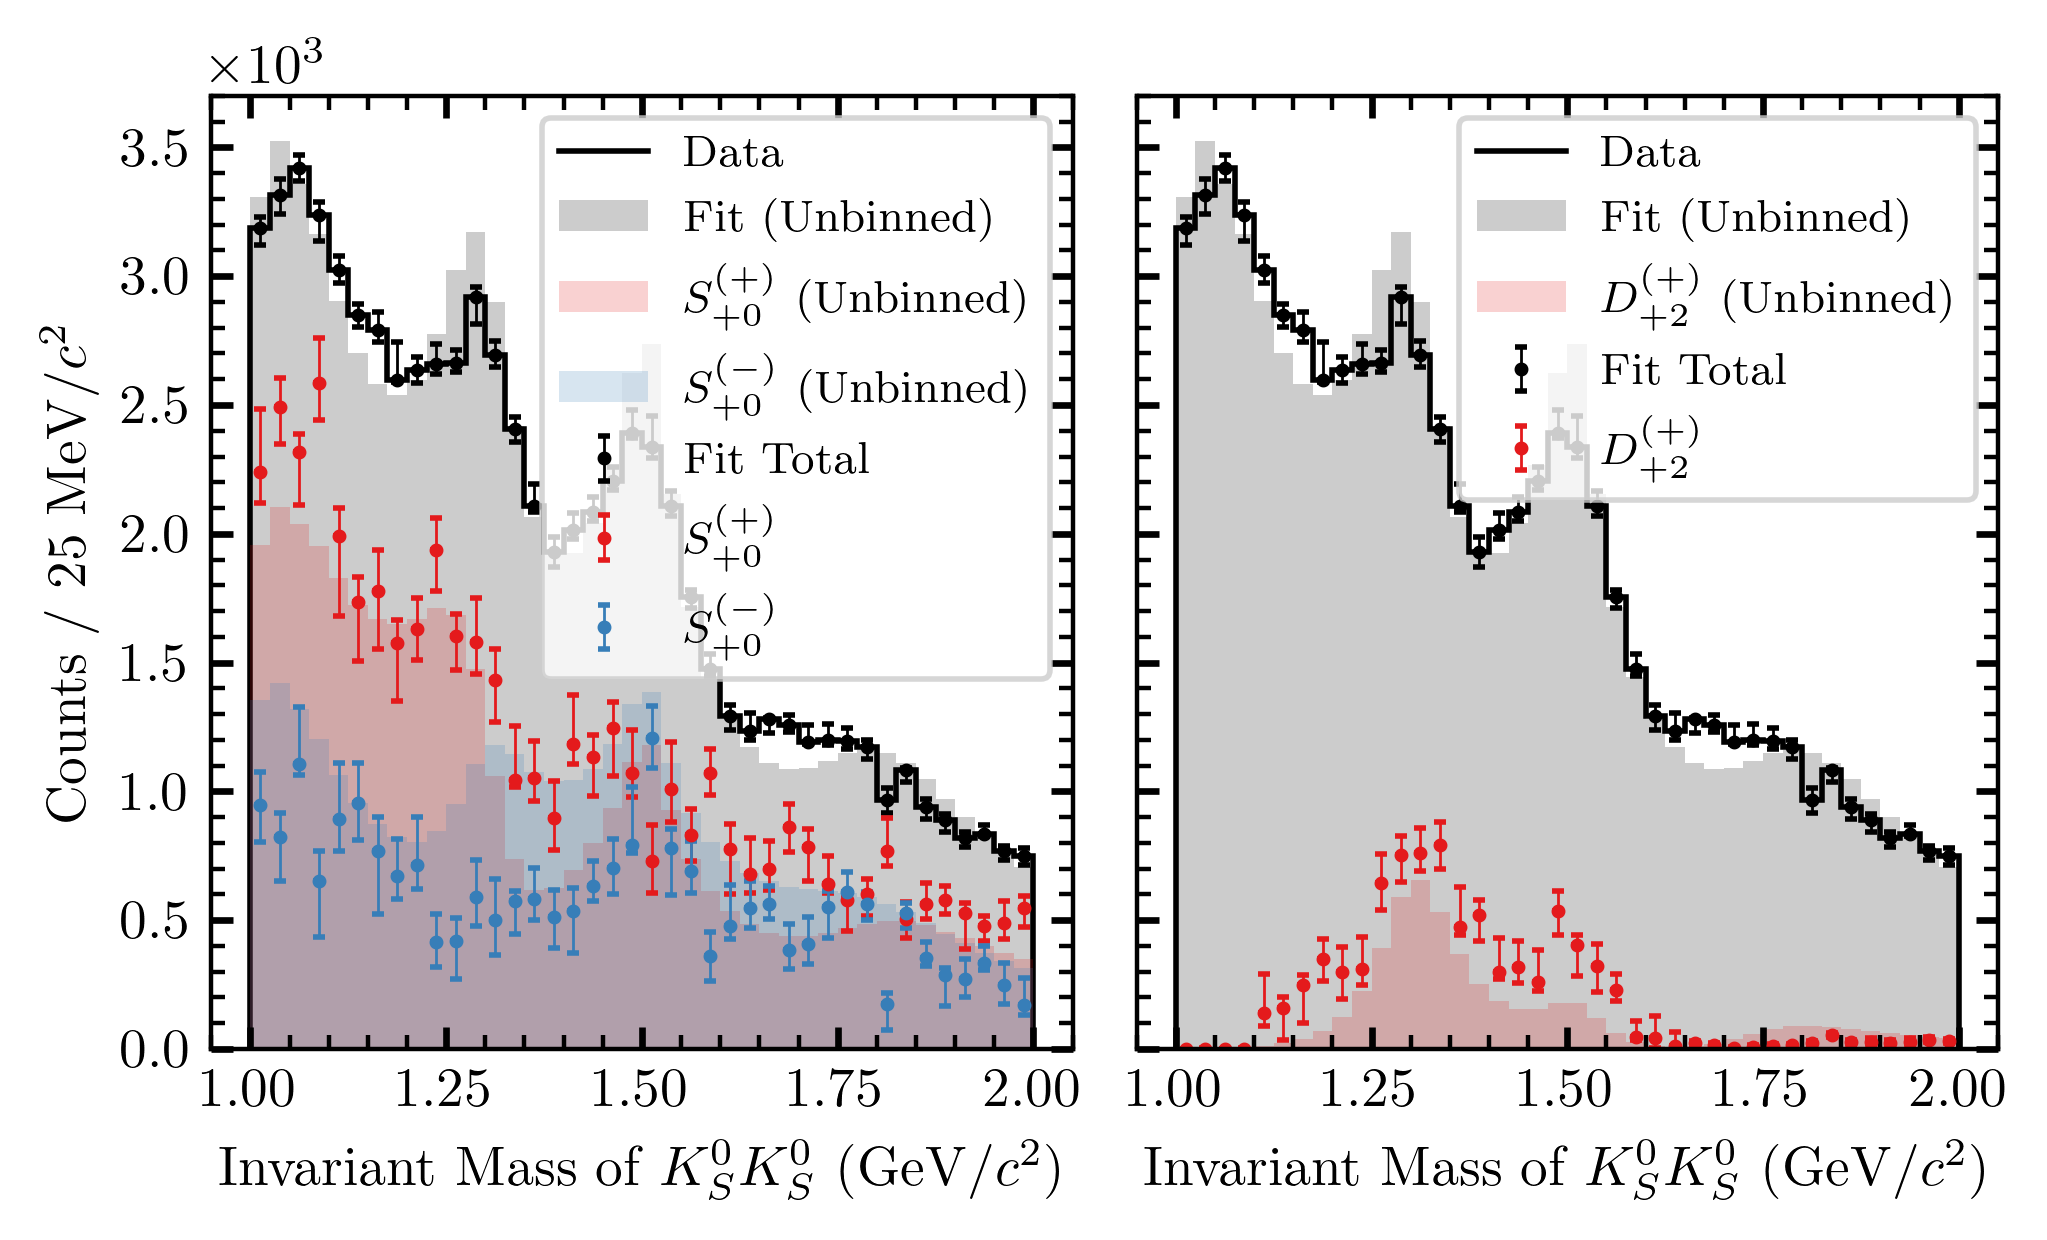
\includegraphics[width=0.8\textwidth]{figures/binned_and_unbinned_fit_chisqdof_3.4_splot_D_1s_2b_phase_factor_waves29099_uncertainty_bootstrap-SE.png}
  \end{center}
  \caption{Mass-independent (binned) and mass-dependent (unbinned) fit of $S_{0}^{(+)}$, $S_{0}^{(-)}$, and $D_{+2}^{(+)}$ waves. Bars on each binned fit point correspond to $68\%$ bias-corrected confidence intervals over $ 30 $ bootstrap iterations.}\label{fig:unbinned-fit-chisqdof-3.4-Spn-D2p}
\end{figure}

\subsection{Guided Fits}\label{sub:guided-fits}

To perform the fits in \Cref{sec:mass-independent-fits,sec:mass-dependent-fits}, we must pick a starting position for the minimizer. Because there are so many free parameters\footnote{Seven for the $f_0$, four for the $a_0$, eight for the $f_2$, and four for the $a_2$ $K$-matrix production amplitude, totaling $23$ parameters for the two-wave model and $34$ parameters for the three-wave model}, no way to measure isospin, and interference effects between many overlapping resonances, there is a high potential to find local minima during the fitting process.

One method for raising the chance to find the global minimum is repeating the fit with a randomized starting position. While it is impossible to quantify the number of random restarts needed to find the global minimum, there are several criteria which could be used to estimate how many restarts are required to attain a certain degree of confidence that the remaining number of unseen local minima is below a given threshold~\cite{Dick2014}\footnote{As an interesting historical note, the metric in the cited work uses the Good-Turing estimator, which was used by Turing and Good to estimate probabilities related to the choosing of cipher pages for the Enigma machine in World War II.}. However, we will refrain from using such methods in favor of a procedure which we refer to as a ``guided'' fit. In this method, we assume that the binned fits have some degree of correctness and that the unbinned fits should give approximately the same result in each bin. The ``guided'' procedure is as follows:

First, a binned fit is performed with the desired final set of waves. Bootstrap samples are also evaluated for determining uncertainties. Next, the power set of waves is taken such that every individual wave along with every combination of waves (ignoring the null set) is recorded for every bin, and the standard error on each projected waveset is evaluated from the bootstrap samples in each bin. Next, a minimization is performed using the mass-dependent model. At every step in this minimization, the model is evaluated according to the current parameter space vector $\vec{\beta}$ and each waveset in the power set is projected onto the accepted Monte Carlo, which is binned in mass. The cost function used in determining the next minimization step is then a $\chi^2$-like distance between the mass-dependent model projection and the solution of the binned fit,

\begin{equation}
  \chi^2(\vec{\beta}) = \sum_i^{\mathcal{P}(\text{waves})} \sum_j^{\text{bins}} \frac{(\mathcal{I}_{ij}(\vec{\beta}) - I_{ij})^2}{\sigma_{ij}^2}
\end{equation}
where $\mathcal{I}_{ij}(\vec{\beta})$ is intensity of the $K$-matrix model of the $i$th waveset in the $j$th bin, $I_{ij}$ is the intensity from the binned fit for the $i$th waveset in the $j$th bin, and $\sigma_{ij}$ is the standard error (according to \Cref{eq:bootstrap-standard-error}) of the $i$th waveset in the $j$th bin.

This method can also be thought of as minimizing the distance between the binned and unbinned fits when projected into their individual waves. However, since these waves might interfere with each other, projecting the waves by themselves will not fully constrain the problem, while projecting all of the waves and all of their combinations (the power set) will. There are some redundancies in doing this. For instance, the combination of two non-interfering waves like the $S_0^{(-)}$ and $D_2^{(+)}$ is linearly dependent on the magnitudes of the individual waves, but the power set ensures all combinations are given the same statistical weight in the cost function, regardless of their degree of interference.

After this minimization is performed (which we refer to as the ``guided'' step), we still must perform a final mass-dependent minimization, since we wish to fit our model to the data and not just to another fit of the data. We treat the result of the guided step as the initial point for this final minimization.

The results of this method are interesting. \Cref{fig:guided-fit-chisqdof-3.4-Sp-D2p,fig:guided-fit-chisqdof-3.4-Spn-D2p} display the state of each fit immediately after the guided step terminates. We can see that while the fit total tends to undershoot the data, each individual wave matches the binned fit projection incredibly well (by construction). Using these states as the initial position of the formal minimization, we obtain the results shown in \Cref{fig:unbinned-guided-fit-chisqdof-3.4-Sp-D2p,fig:unbinned-guided-fit-chisqdof-3.4-Spn-D2p}.

\begin{figure}
  \begin{center}
    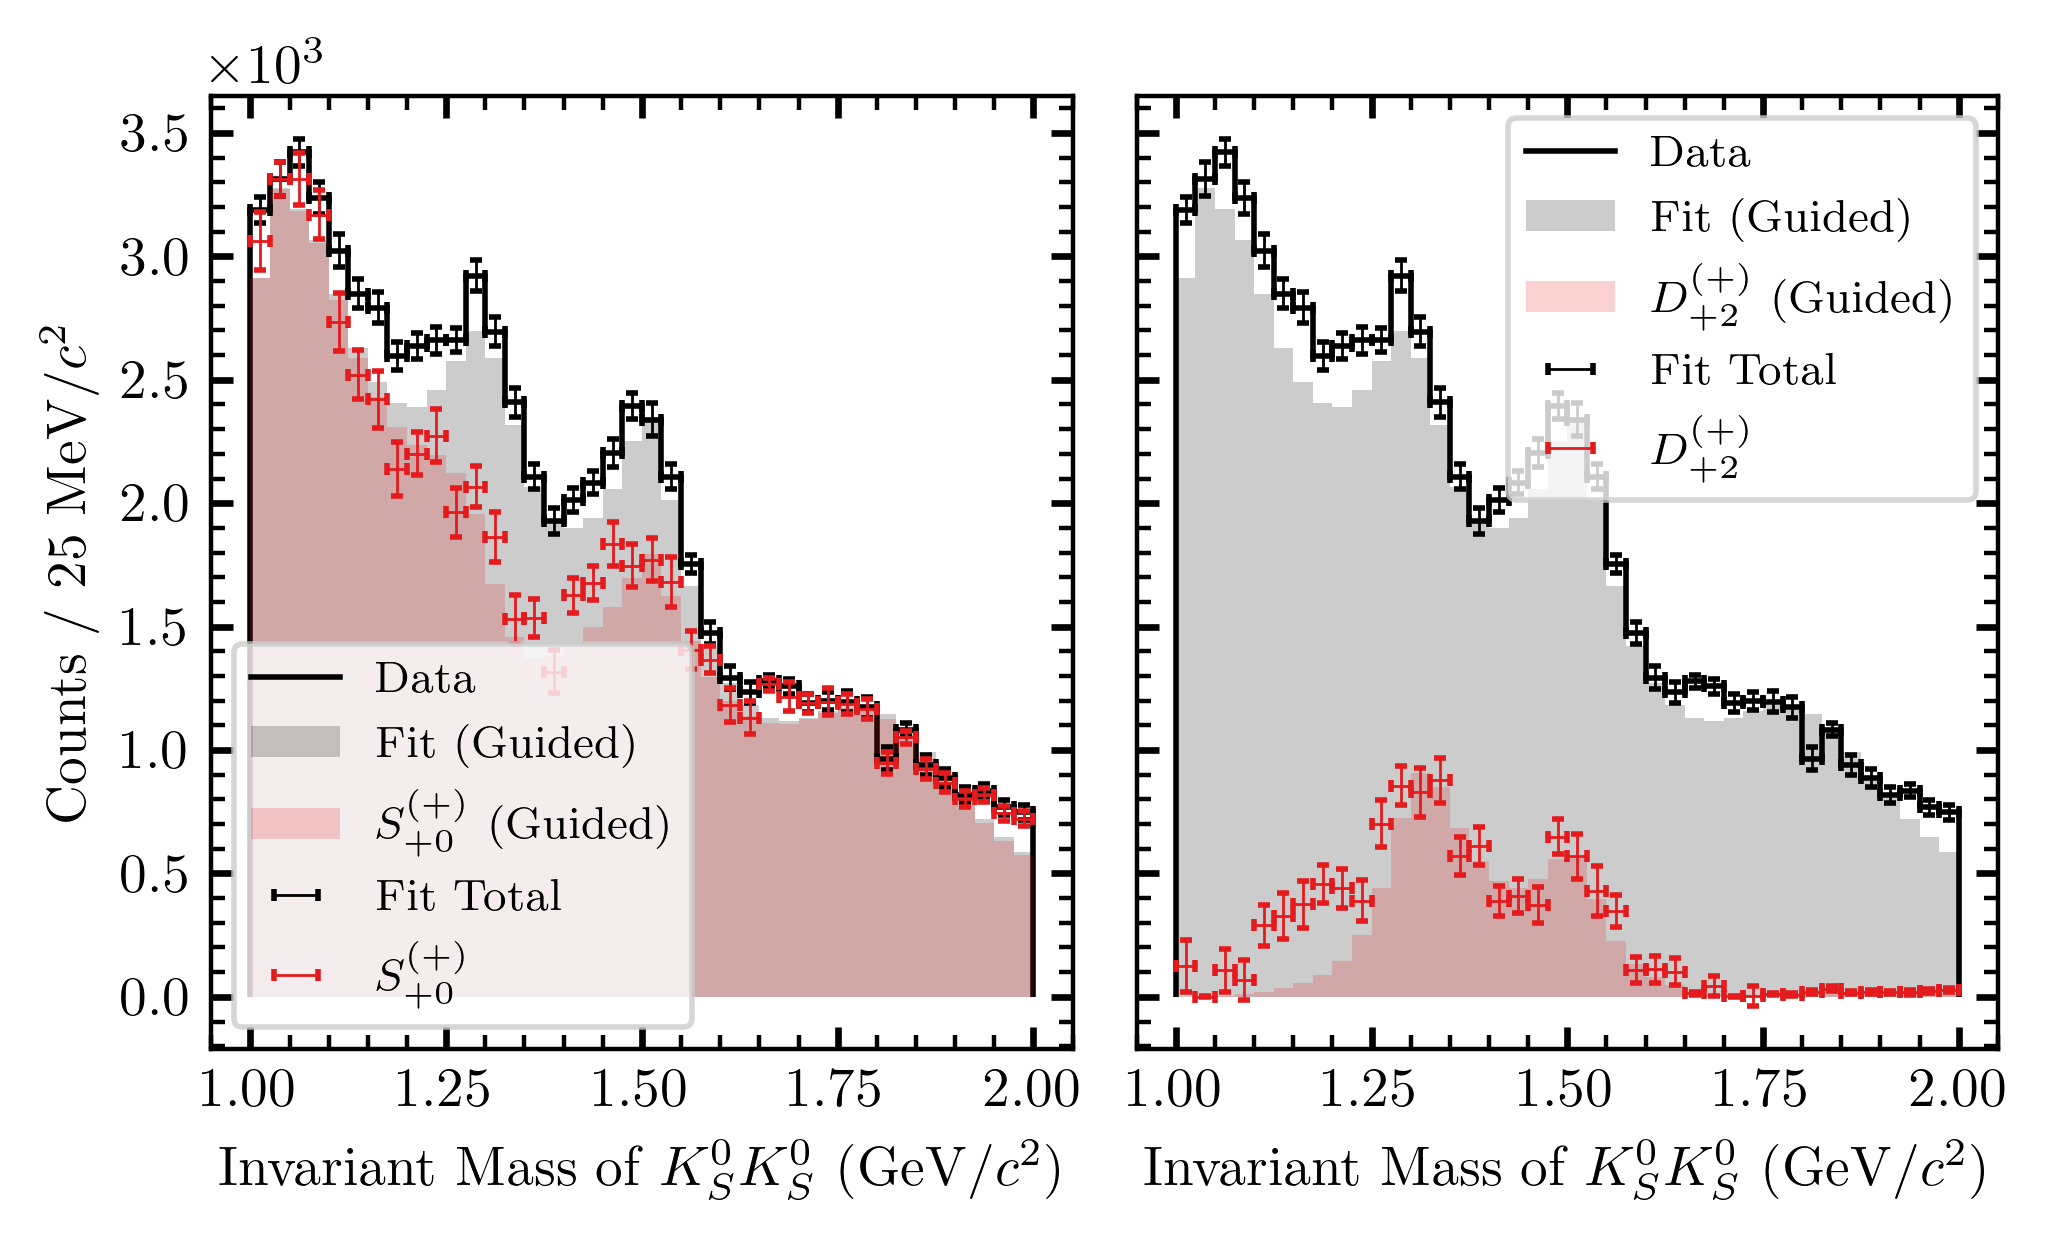
\includegraphics[width=0.8\textwidth]{figures/guided_fit_chisqdof_3.4_splot_D_1s_2b_phase_factor_waves491_uncertainty_bootstrap-SE.png}
  \end{center}
  \caption{The state of the guided fit to $S_{0}^{(+)}$ and $D_{+2}^{(+)}$ waves after the guided step. Bars on the fit points correspond to the standard error on the intensity from $ 30 $ bootstrap samples.}\label{fig:guided-fit-chisqdof-3.4-Sp-D2p}
\end{figure}

\begin{figure}
  \begin{center}
    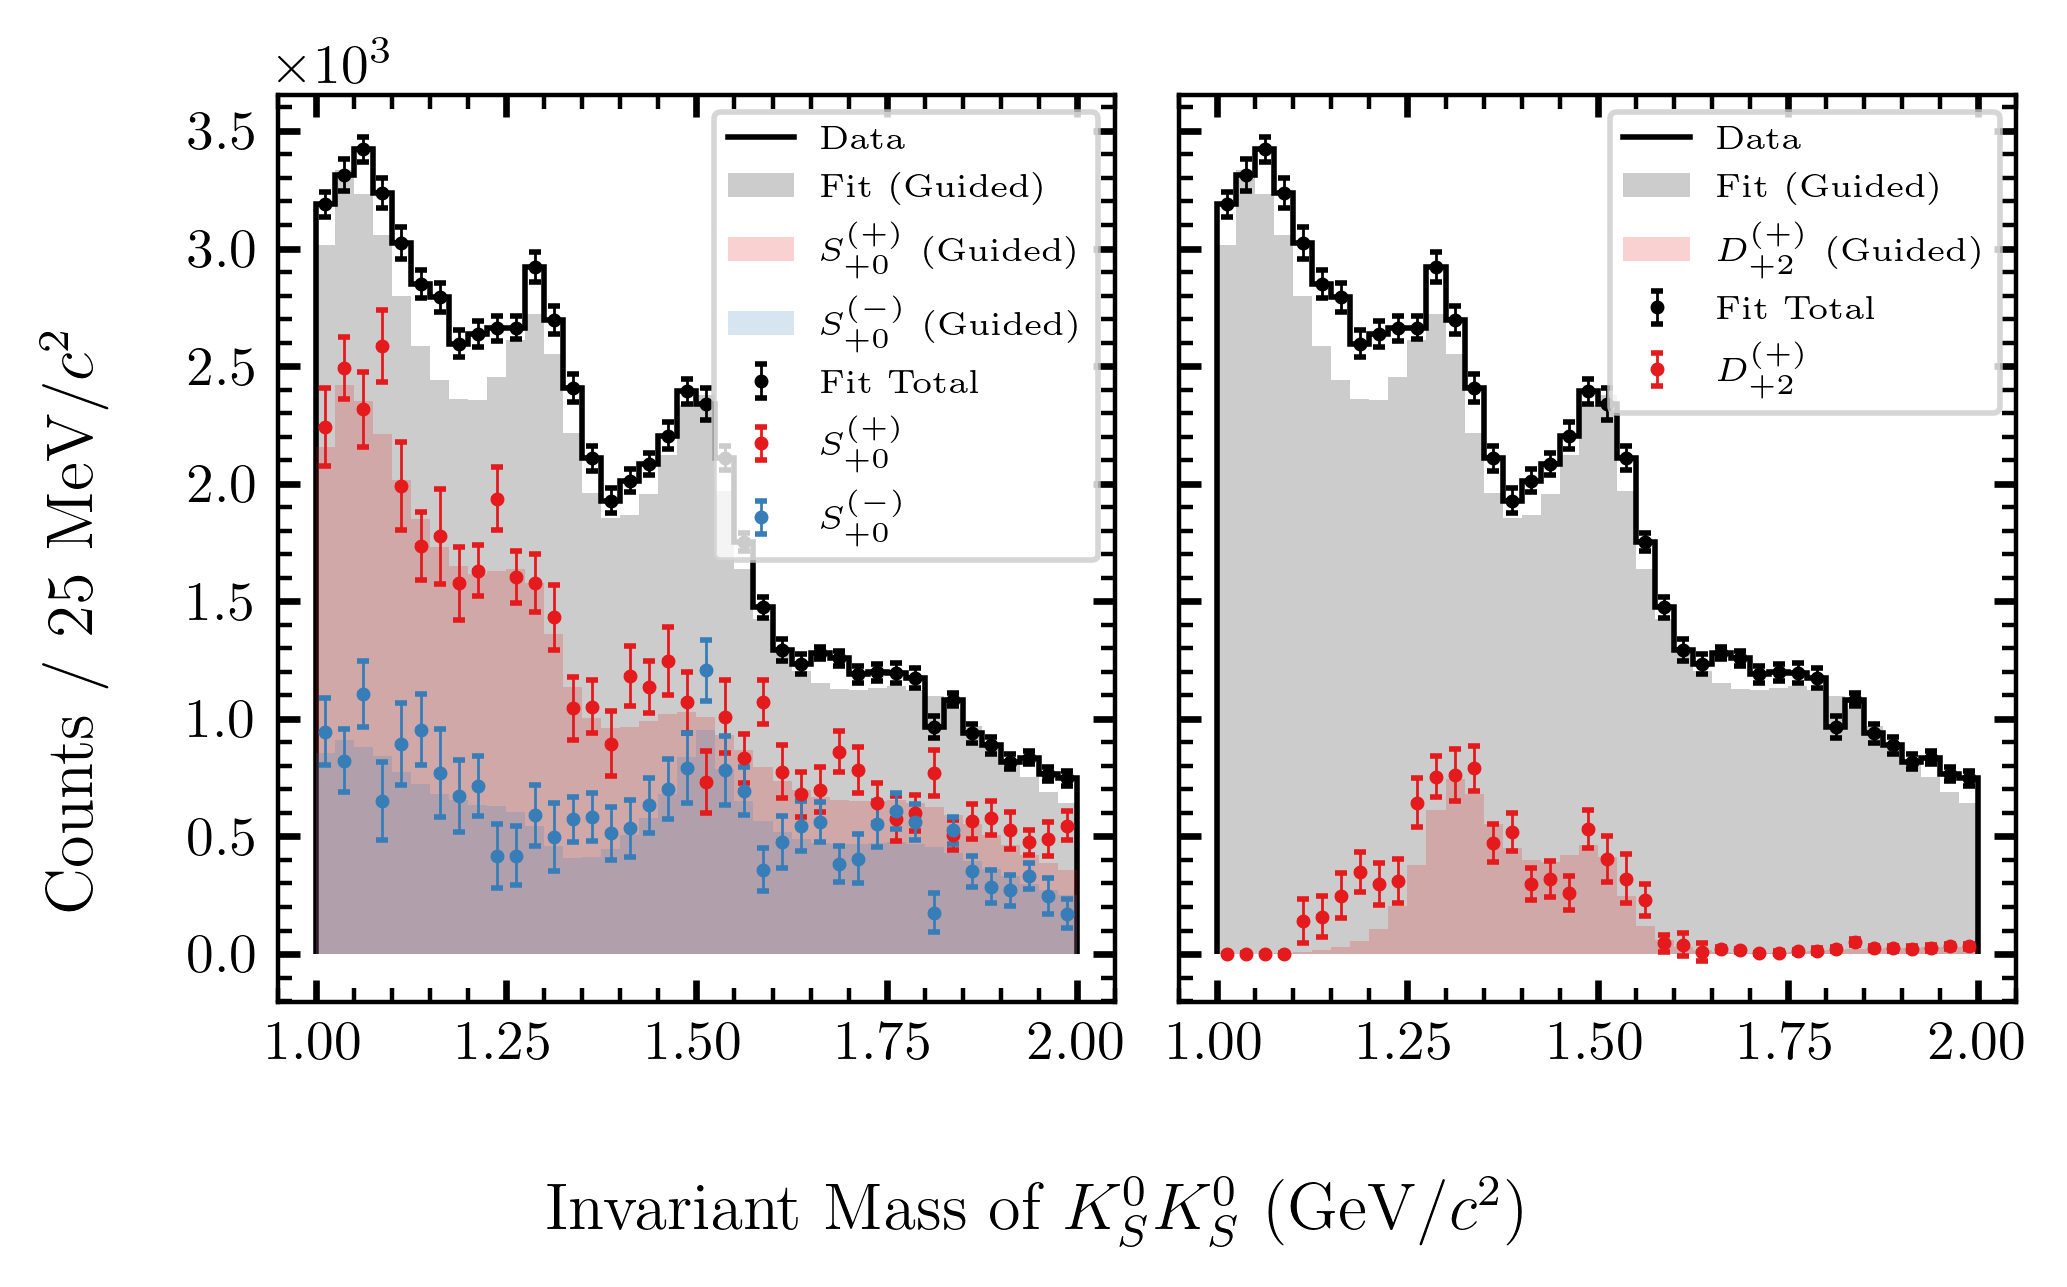
\includegraphics[width=0.8\textwidth]{figures/guided_fit_chisqdof_3.4_splot_D_1s_2b_phase_factor_waves29099_uncertainty_bootstrap-SE.png}
  \end{center}
  \caption{The state of the guided fit to $S_{0}^{(+)}$, $S_{0}^{(-)}$, and $D_{+2}^{(+)}$ waves after the guided step. Bars on the fit points correspond to the standard error on the intensity from $ 30 $ bootstrap samples.}\label{fig:guided-fit-chisqdof-3.4-Spn-D2p}
\end{figure}

\begin{figure}
  \begin{center}                                                                                                                                                                                                                                                                                                                                                                                                                                                                                                                                                                                                                                                                                                                                                                                                                                                                                     e
    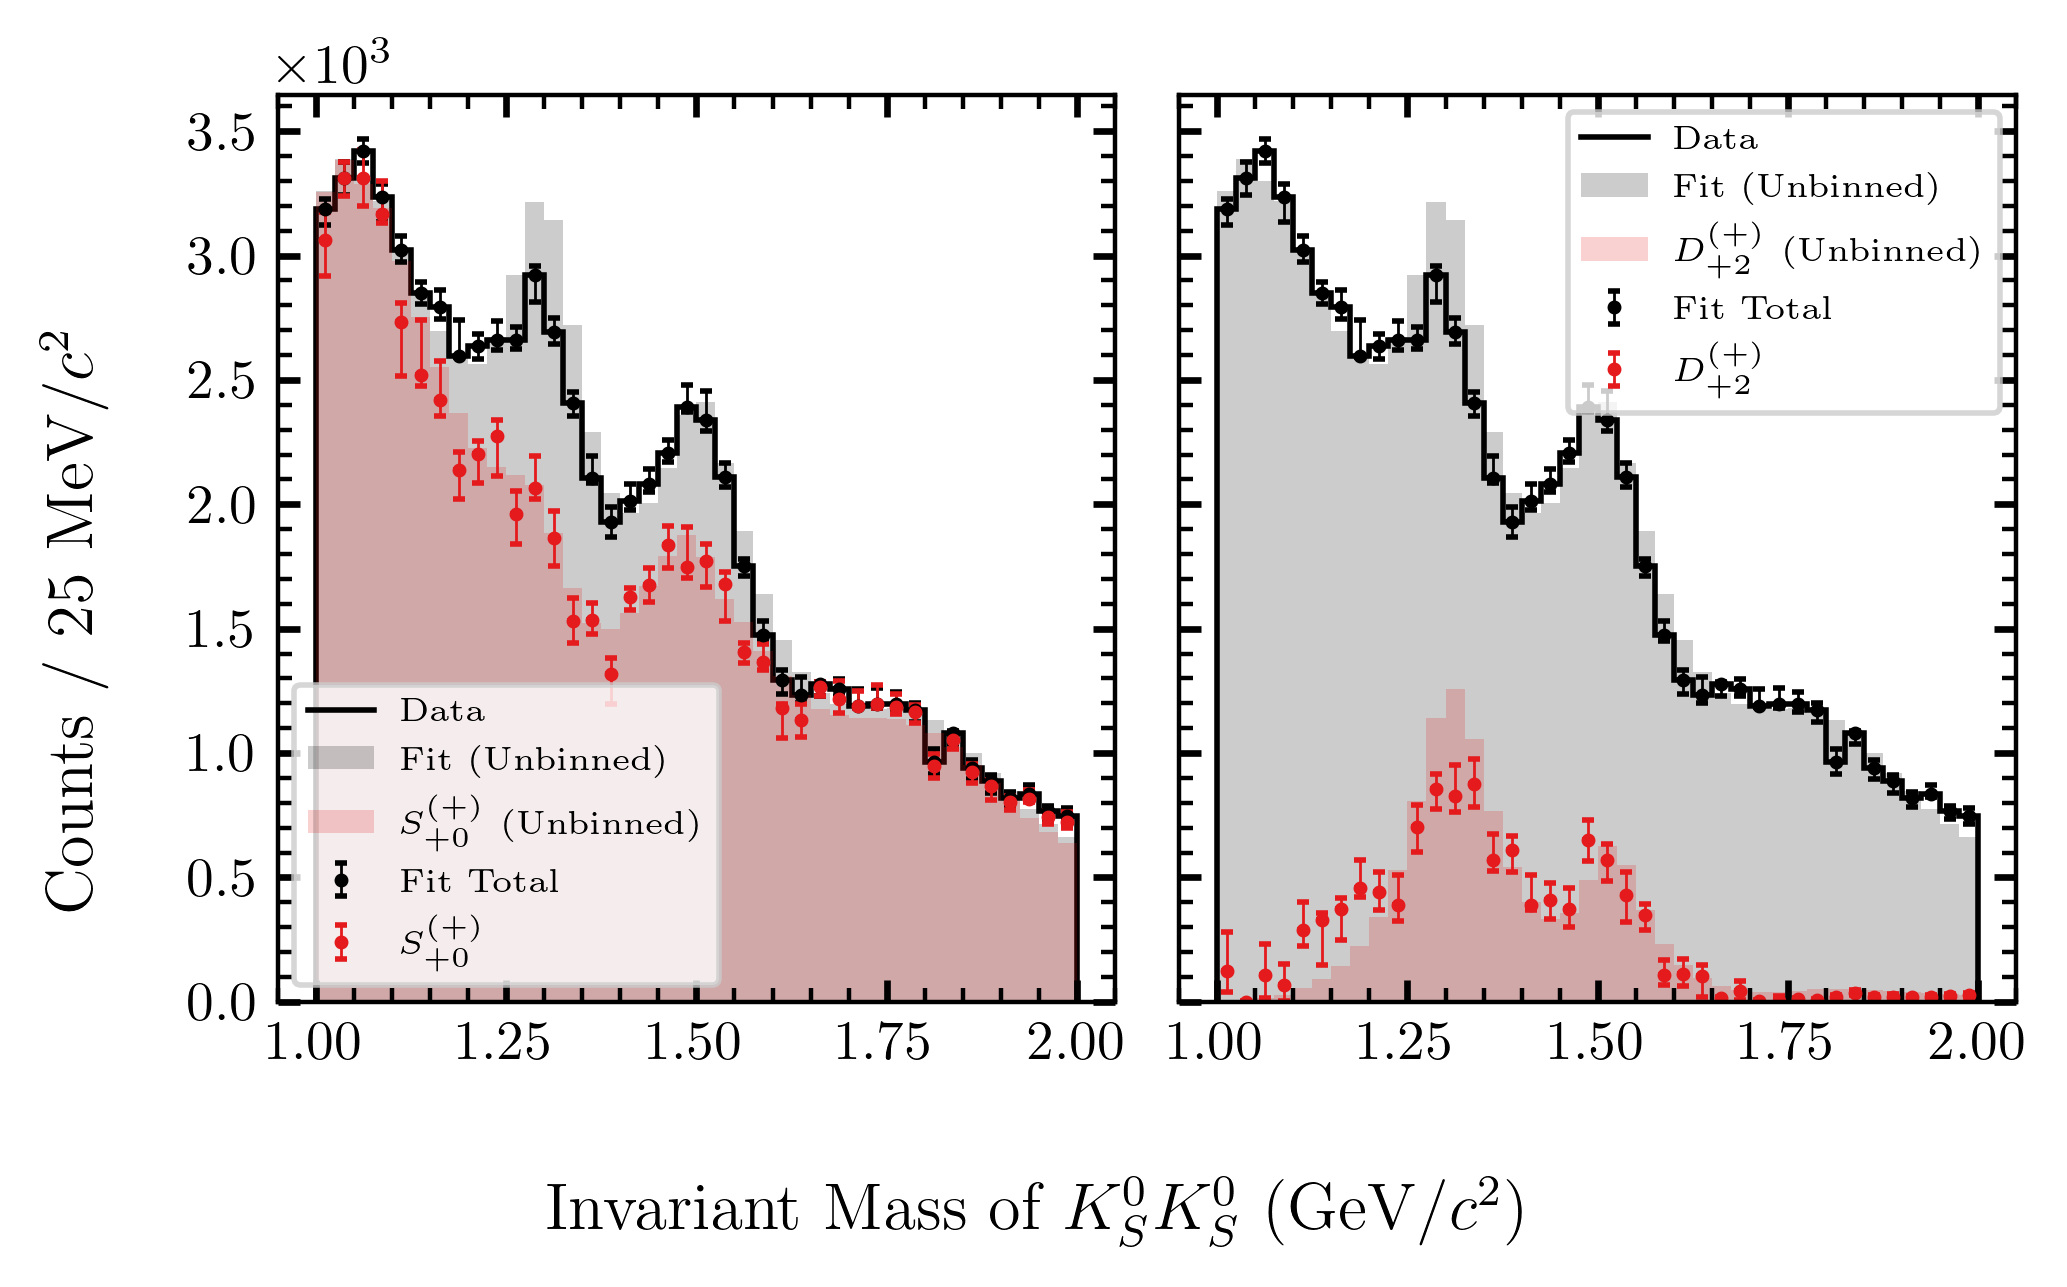
\includegraphics[width=0.8\textwidth]{figures/binned_and_unbinned_fit_chisqdof_3.4_splot_D_1s_2b_guided_phase_factor_waves491_uncertainty_bootstrap-SE.png}
  \end{center}
  \caption{Mass-independent (binned) and mass-dependent (unbinned, guided) fit of $S_{0}^{(+)}$ and $D_{+2}^{(+)}$ waves. Bars on each binned fit point correspond to the standard error on the intensity from $ 30 $ bootstrap iterations.}\label{fig:unbinned-guided-fit-chisqdof-3.4-Sp-D2p}
\end{figure}

\begin{figure}
  \begin{center}
    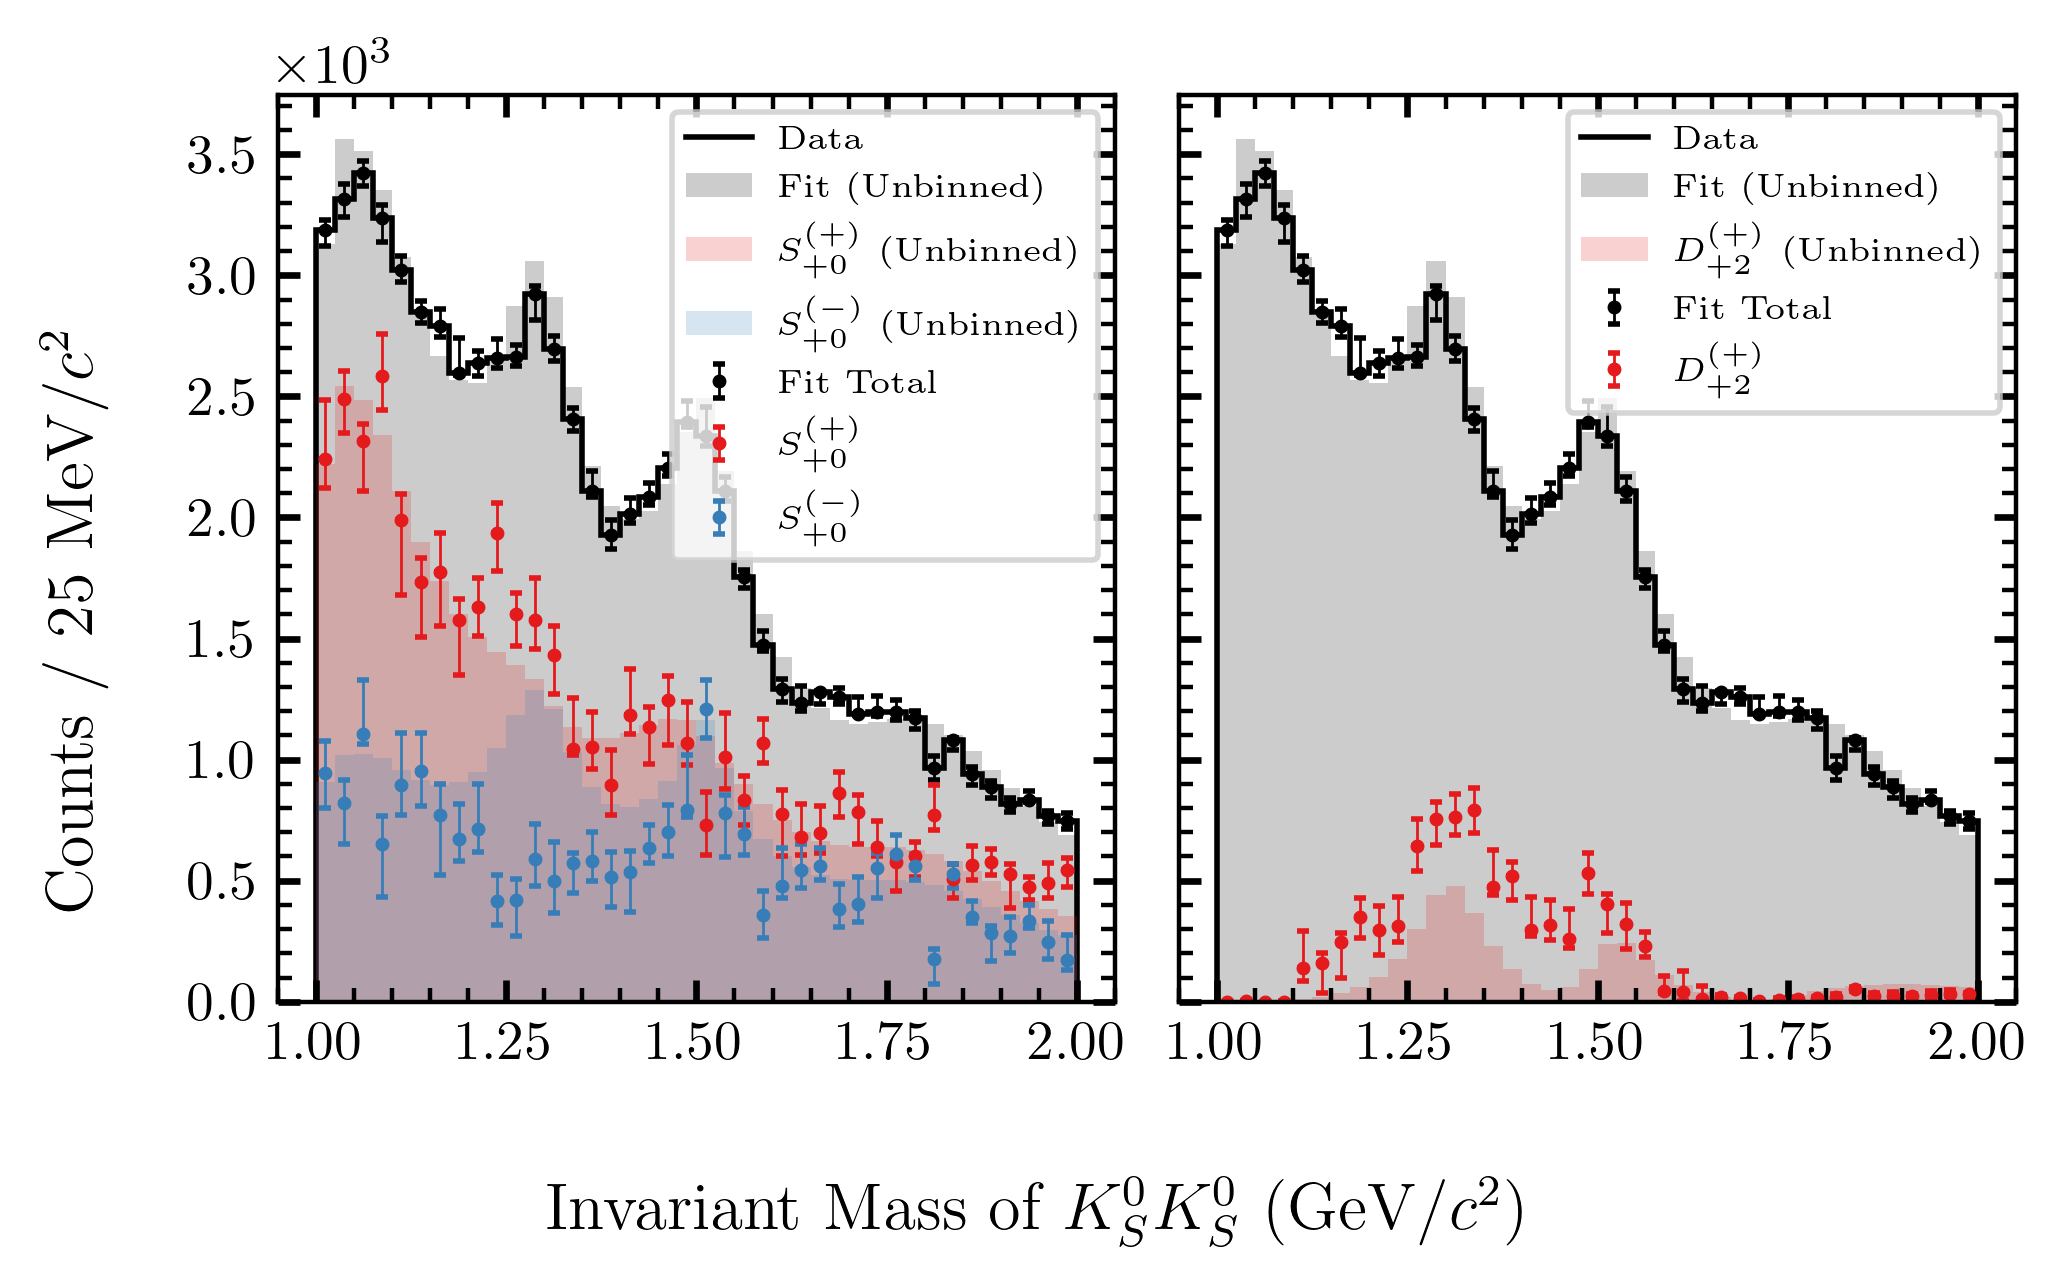
\includegraphics[width=0.8\textwidth]{figures/binned_and_unbinned_fit_chisqdof_3.4_splot_D_1s_2b_guided_phase_factor_waves29099_uncertainty_bootstrap-SE.png}
  \end{center}
  \caption{Mass-independent (binned) and mass-dependent (unbinned, guided) fit of $S_{0}^{(+)}$, $S_{0}^{(-)}$, and $D_{+2}^{(+)}$ waves. Bars on each binned fit point correspond to $68\%$ bias-corrected confidence intervals over $ 30 $ bootstrap iterations.}\label{fig:unbinned-guided-fit-chisqdof-3.4-Spn-D2p}
\end{figure}

Both of these fits appear to be improvements over the local minima found in the previous section, although there are still deviations from the binned fits. The $D$-wave is much closer to that of the binned fit in \Cref{fig:unbinned-guided-fit-chisqdof-3.4-Sp-D2p}, and the region at threshold is more consistent in \Cref{fig:unbinned-guided-fit-chisqdof-3.4-Spn-D2p}. However, this second fit with three waves is still lacking in the total $D$-wave contribution, and the region at $\SI{1.25}{\giga\electronvolt}$ in the $S$-wave still shows a negative-reflectivity contribution where none exists in the binned fit, as well as a missing positive-reflectivity peak in the same mass range. This region is more faithfully modeled in the guided step, but the minimizer drifts from this solution when the guided objective is no longer present. This could possibly be due to the unmodeled $D$-wave contribution in this part of the spectrum, or it could simply be a local minimum of the parameter space. Nonetheless, these guided fits provide the best and final model of the data which will be presented in this thesis.

\section{Systematic Studies}\label{sec:systematic-studies}

We now bring our attention back to the selections which were made in \Cref{sec:data-selection}, particularly the choice to cut on the $\chi^2_\nu$ value from the kinematic fit. The choice of $\chi^2_\nu = 3.4$ as the cut value was motivated by a maximally informed decision boundary. We will not investigate the effect this cut value has on our analysis.

To do this, we will select four new cut values spaced by a unit of $\chi^2_\nu$, two on either side of the chosen value, i.e. $\chi^2_\nu \in \{1.4, 2.4, 3.4, 4.4, 5.4\}$. We are not extracting a quantitative value from this analysis, so we will just observe the fits done in the prior section under these different cut values. The $A2$ sPlot weighting method will still be used, but the distribution used for the signal and the slopes used to initialize the background in the fit will be sourced from Monte Carlo with these different cut values. The results of these fits can be seen in \Cref{fig:binned-fit-all-Sp-D0p,fig:binned-fit-all-Sp-D1p,fig:binned-fit-all-Sp-D2p,fig:binned-fit-all-Spn-D2p,fig:unbinned-fit-all-Sp-D2p,fig:unbinned-fit-all-Spn-D2p,fig:guided-fit-all-Sp-D2p,fig:guided-fit-all-Spn-D2p,fig:unbinned-guided-fit-all-Sp-D2p,fig:unbinned-guided-fit-all-Spn-D2p}. From a cursory examination of these results, it seems like the selection on $\chi^2_\nu$ has very little effect on the overall shape of each wave. Examining \Cref{fig:binned-fit-all-Sp-D0p,fig:binned-fit-all-Sp-D1p}, this selection does not seem to strengthen or diminish contributions from other $D$-wave projections. \Cref{fig:binned-fit-all-Sp-D2p,fig:binned-fit-all-Spn-D2p} also contain similar distributions at all cut values, but the relative height of the peak at $\SI{1.5}{\giga\electronvolt}$ and the enhancement near $\SI{1.15}{\giga\electronvolt}$ seems to change slightly with the cut value, favoring the lower-mass peak at higher values of $\chi^2_\nu$. This may indicate that some component of this bump is related to a background which has not been removed, since it shows up more at higher $\chi^2_\nu$, which correspond to lower confidence events.

\begin{figure}[htbp]
    \centering
    \begin{subfigure}{0.45\textwidth}
        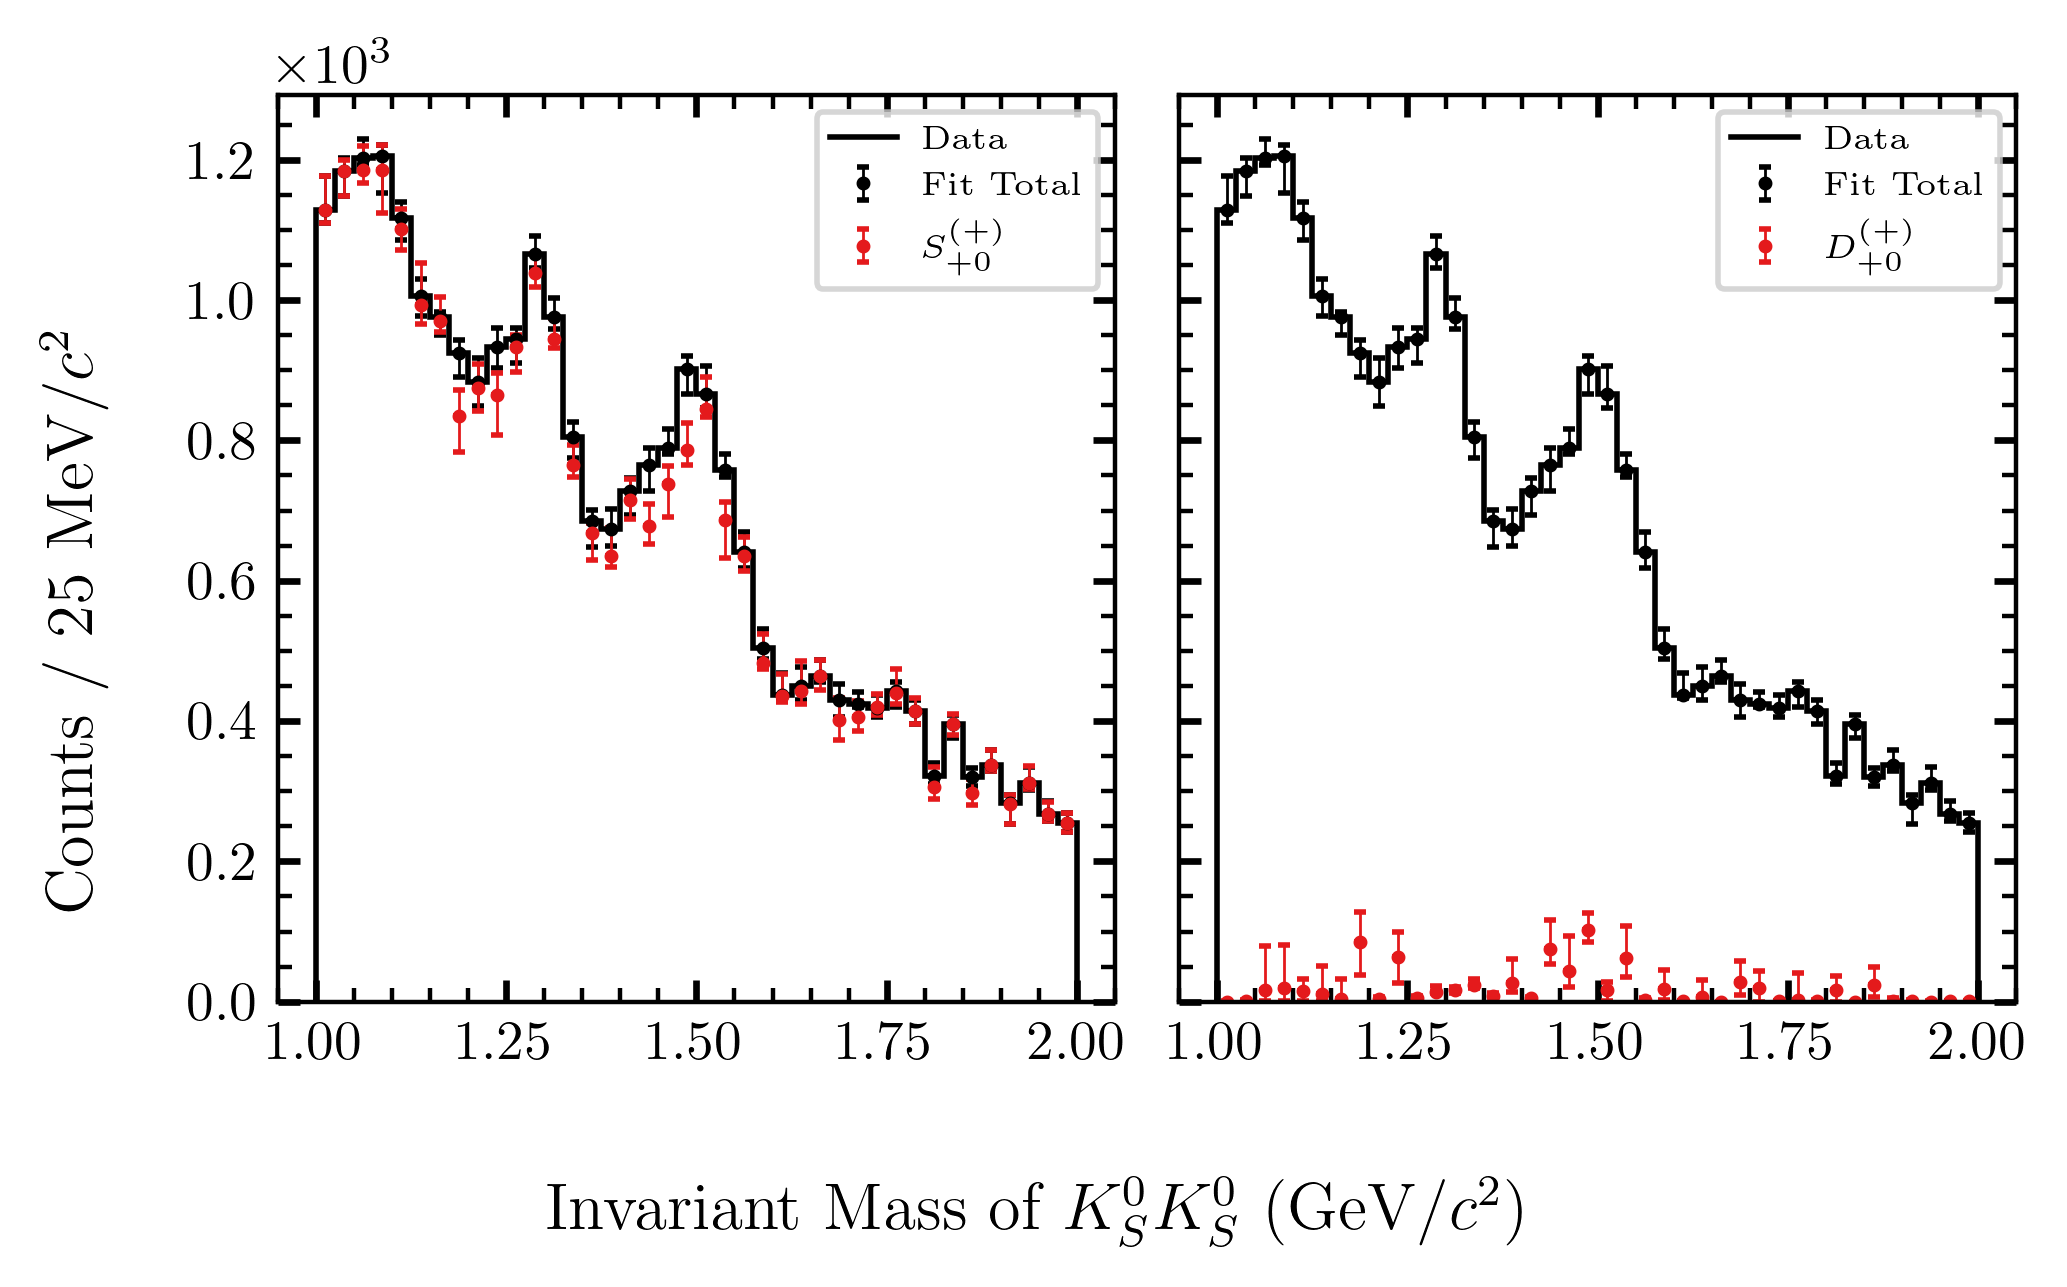
\includegraphics[width=\linewidth]{figures/binned_fit_chisqdof_1.4_splot_D_1s_2b_phase_factor_waves487_uncertainty_bootstrap-CI-BC.png}
        \caption{$\chi^2_\nu < 1.4$}
    \end{subfigure}
    \hfill
    \begin{subfigure}{0.45\textwidth}
        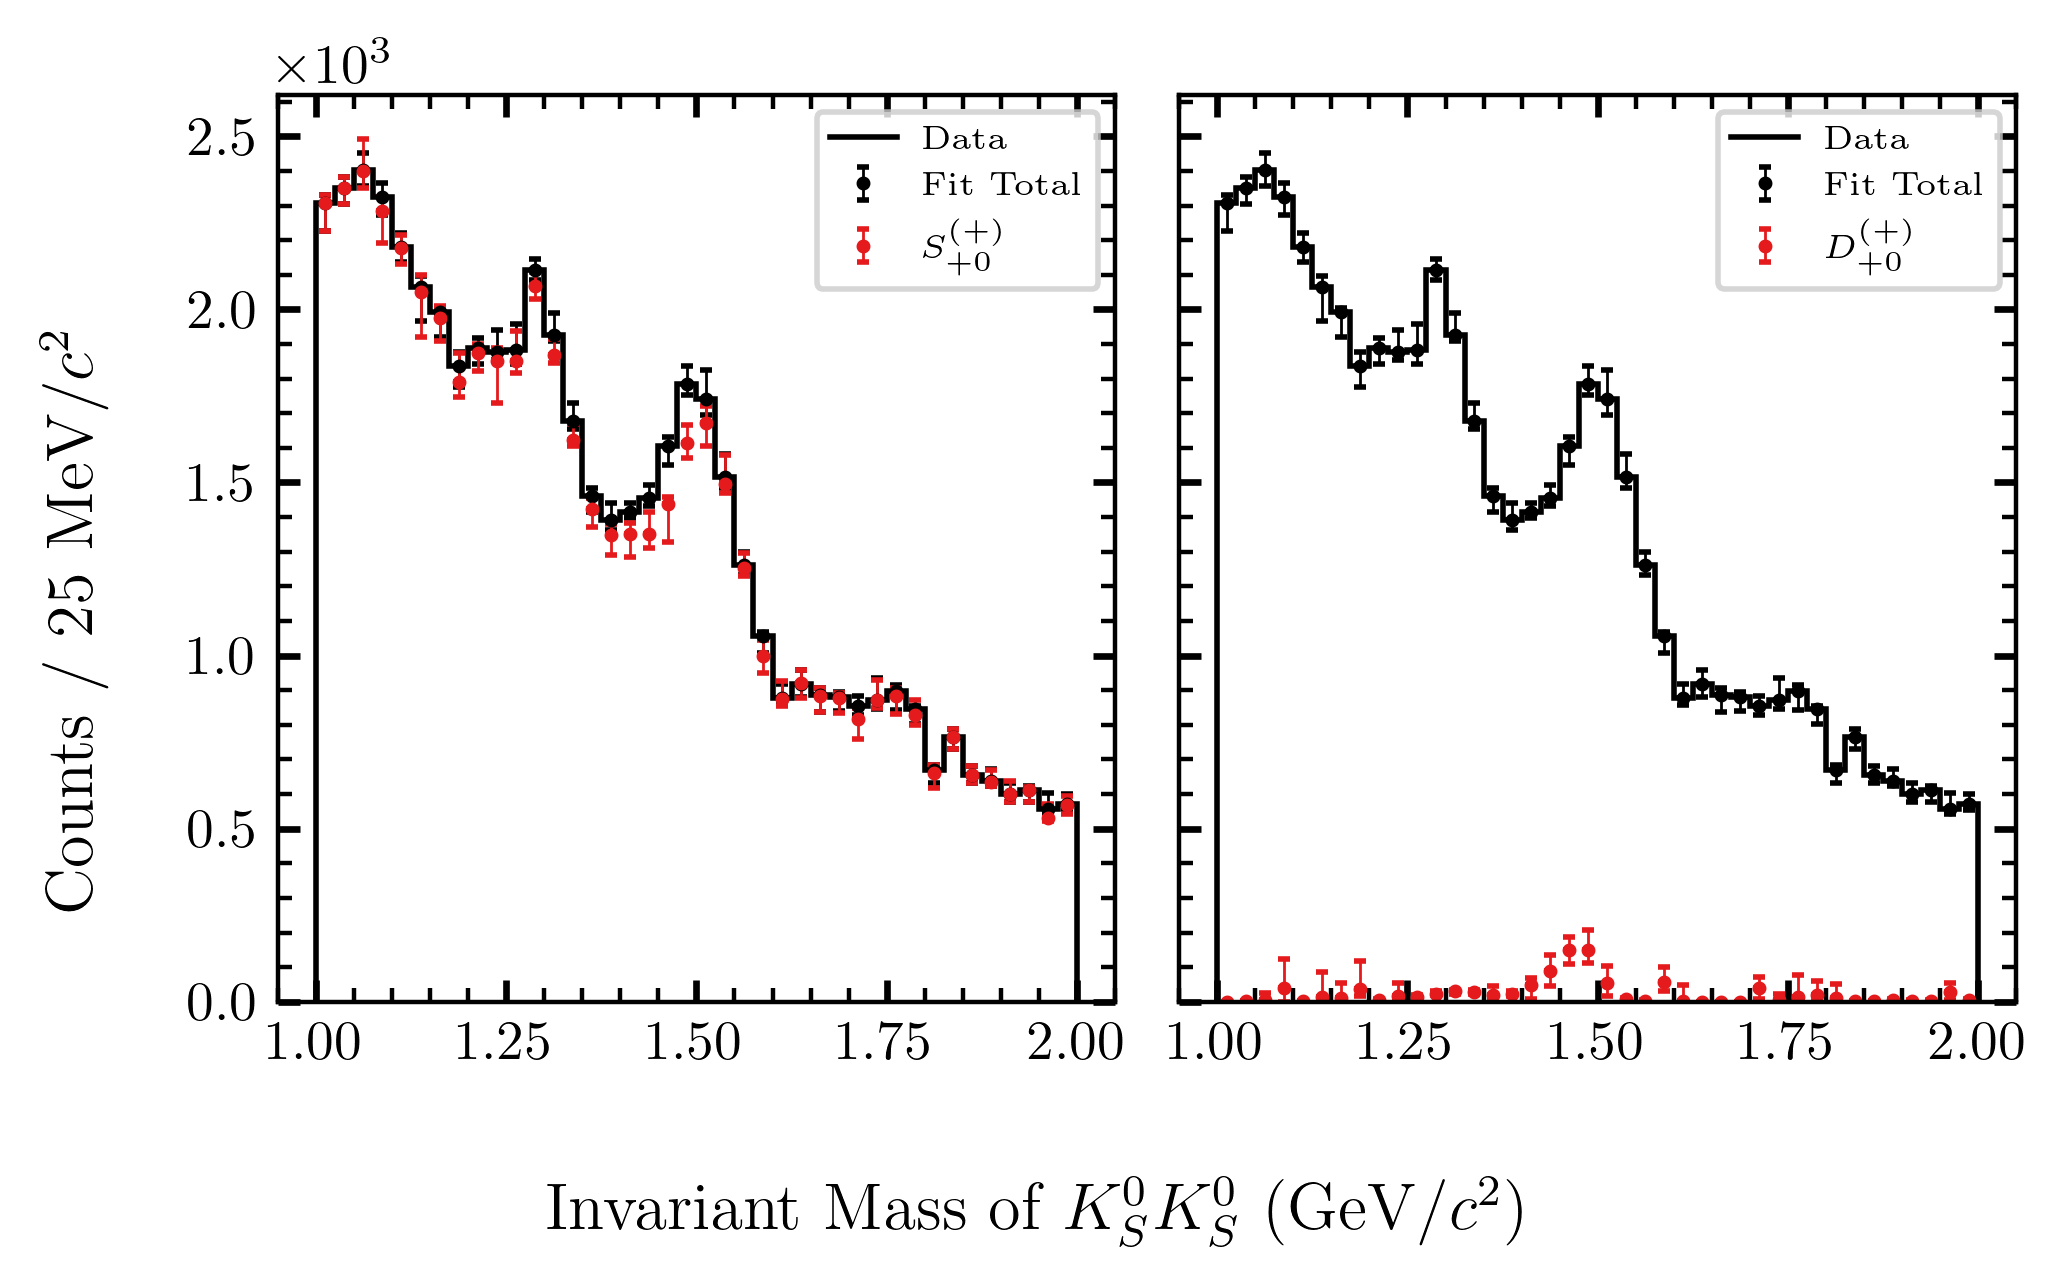
\includegraphics[width=\linewidth]{figures/binned_fit_chisqdof_2.4_splot_D_1s_2b_phase_factor_waves487_uncertainty_bootstrap-CI-BC.png}
        \caption{$\chi^2_\nu < 2.4$}
    \end{subfigure}

    \vspace{1em}

    \begin{subfigure}{0.8\textwidth}
        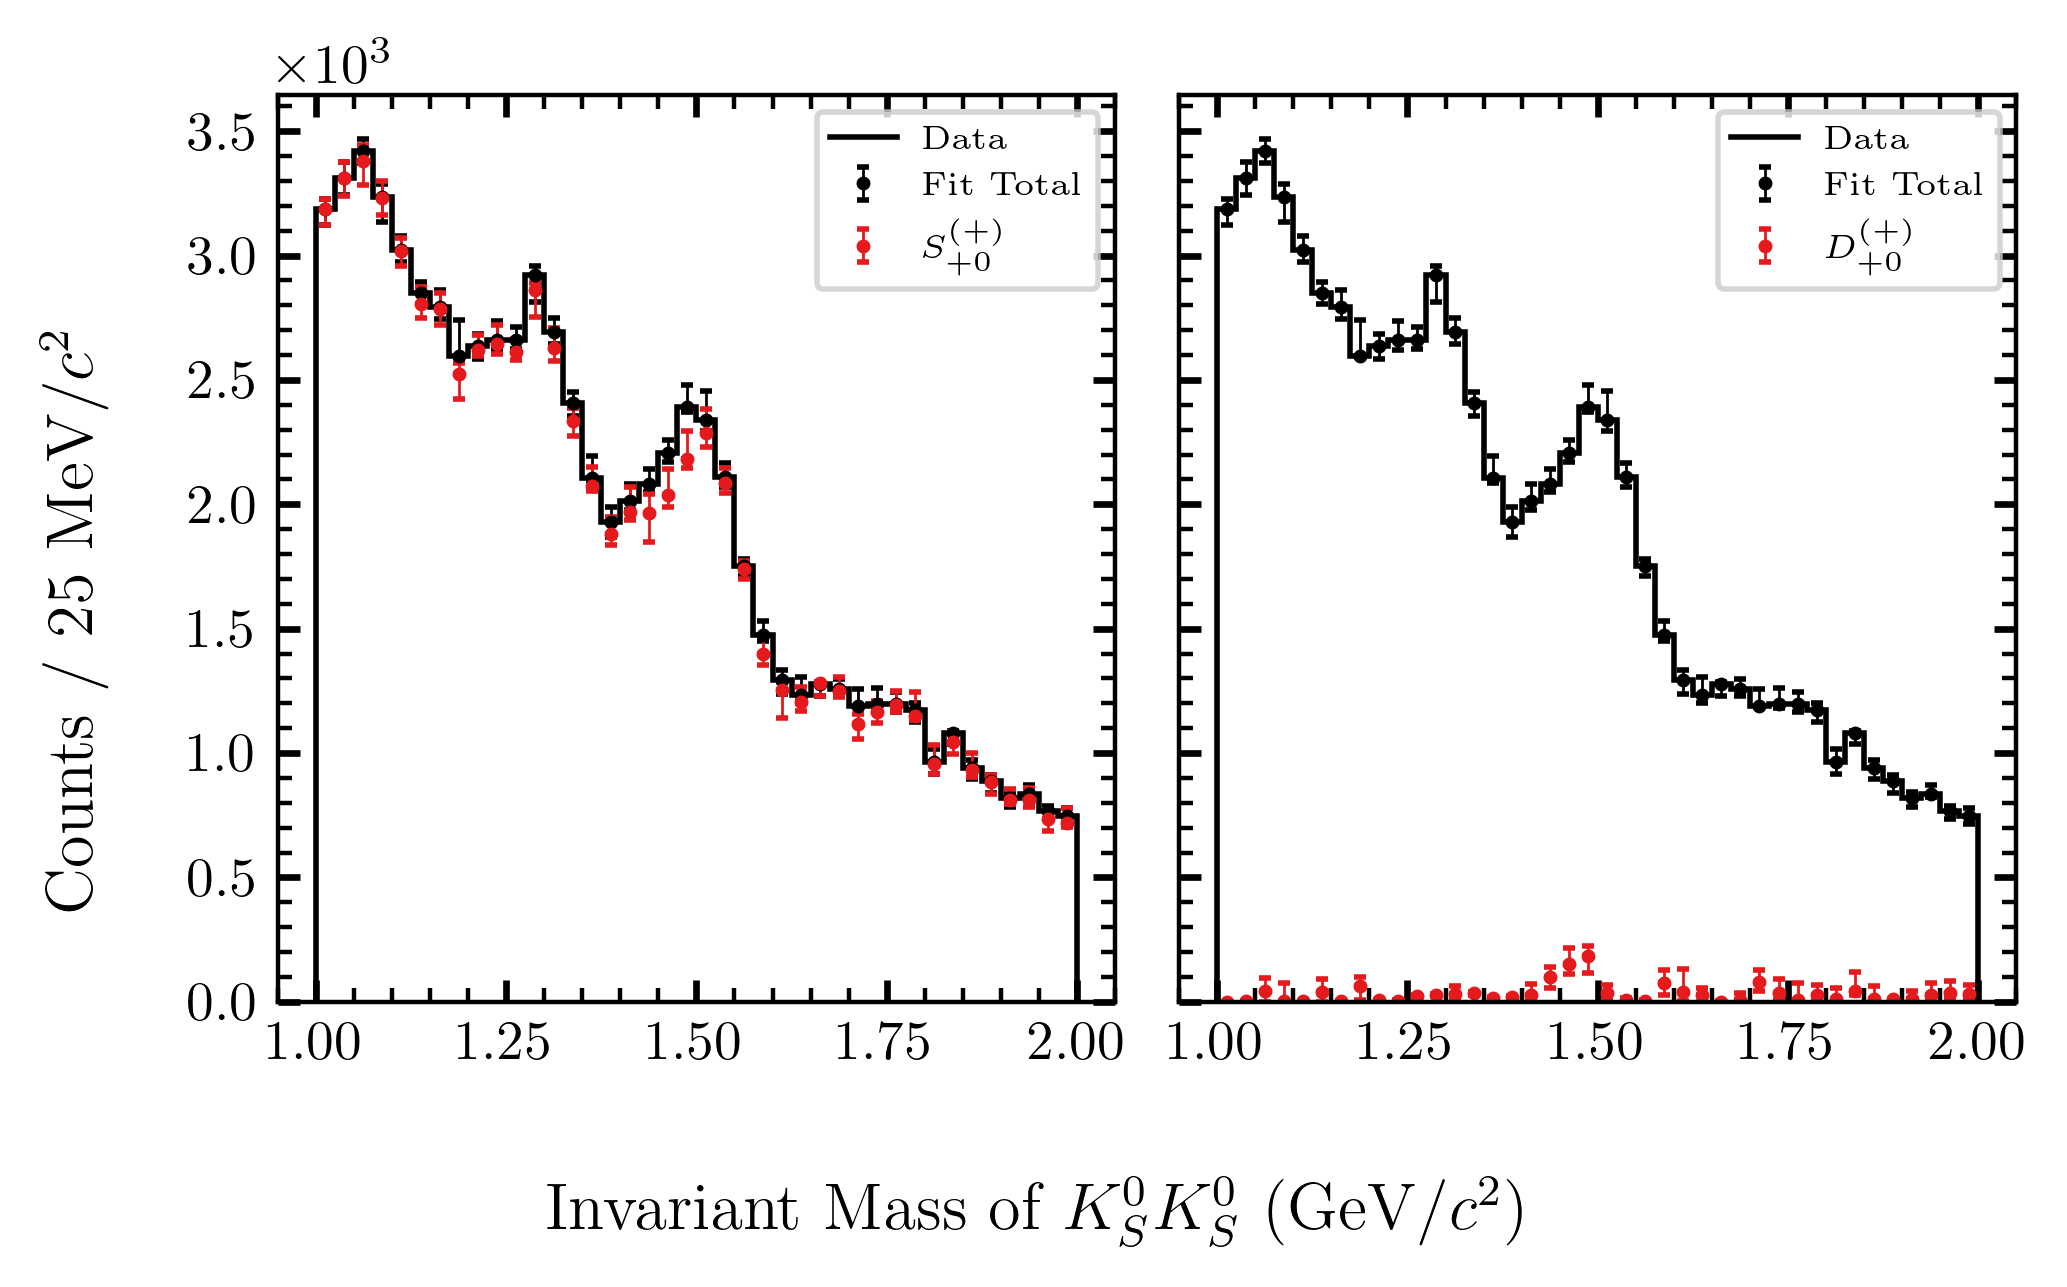
\includegraphics[width=\linewidth]{figures/binned_fit_chisqdof_3.4_splot_D_1s_2b_phase_factor_waves487_uncertainty_bootstrap-CI-BC.png}
        \caption{$\chi^2_\nu < 3.4$}
    \end{subfigure}

    \vspace{1em}

    \begin{subfigure}{0.45\textwidth}
        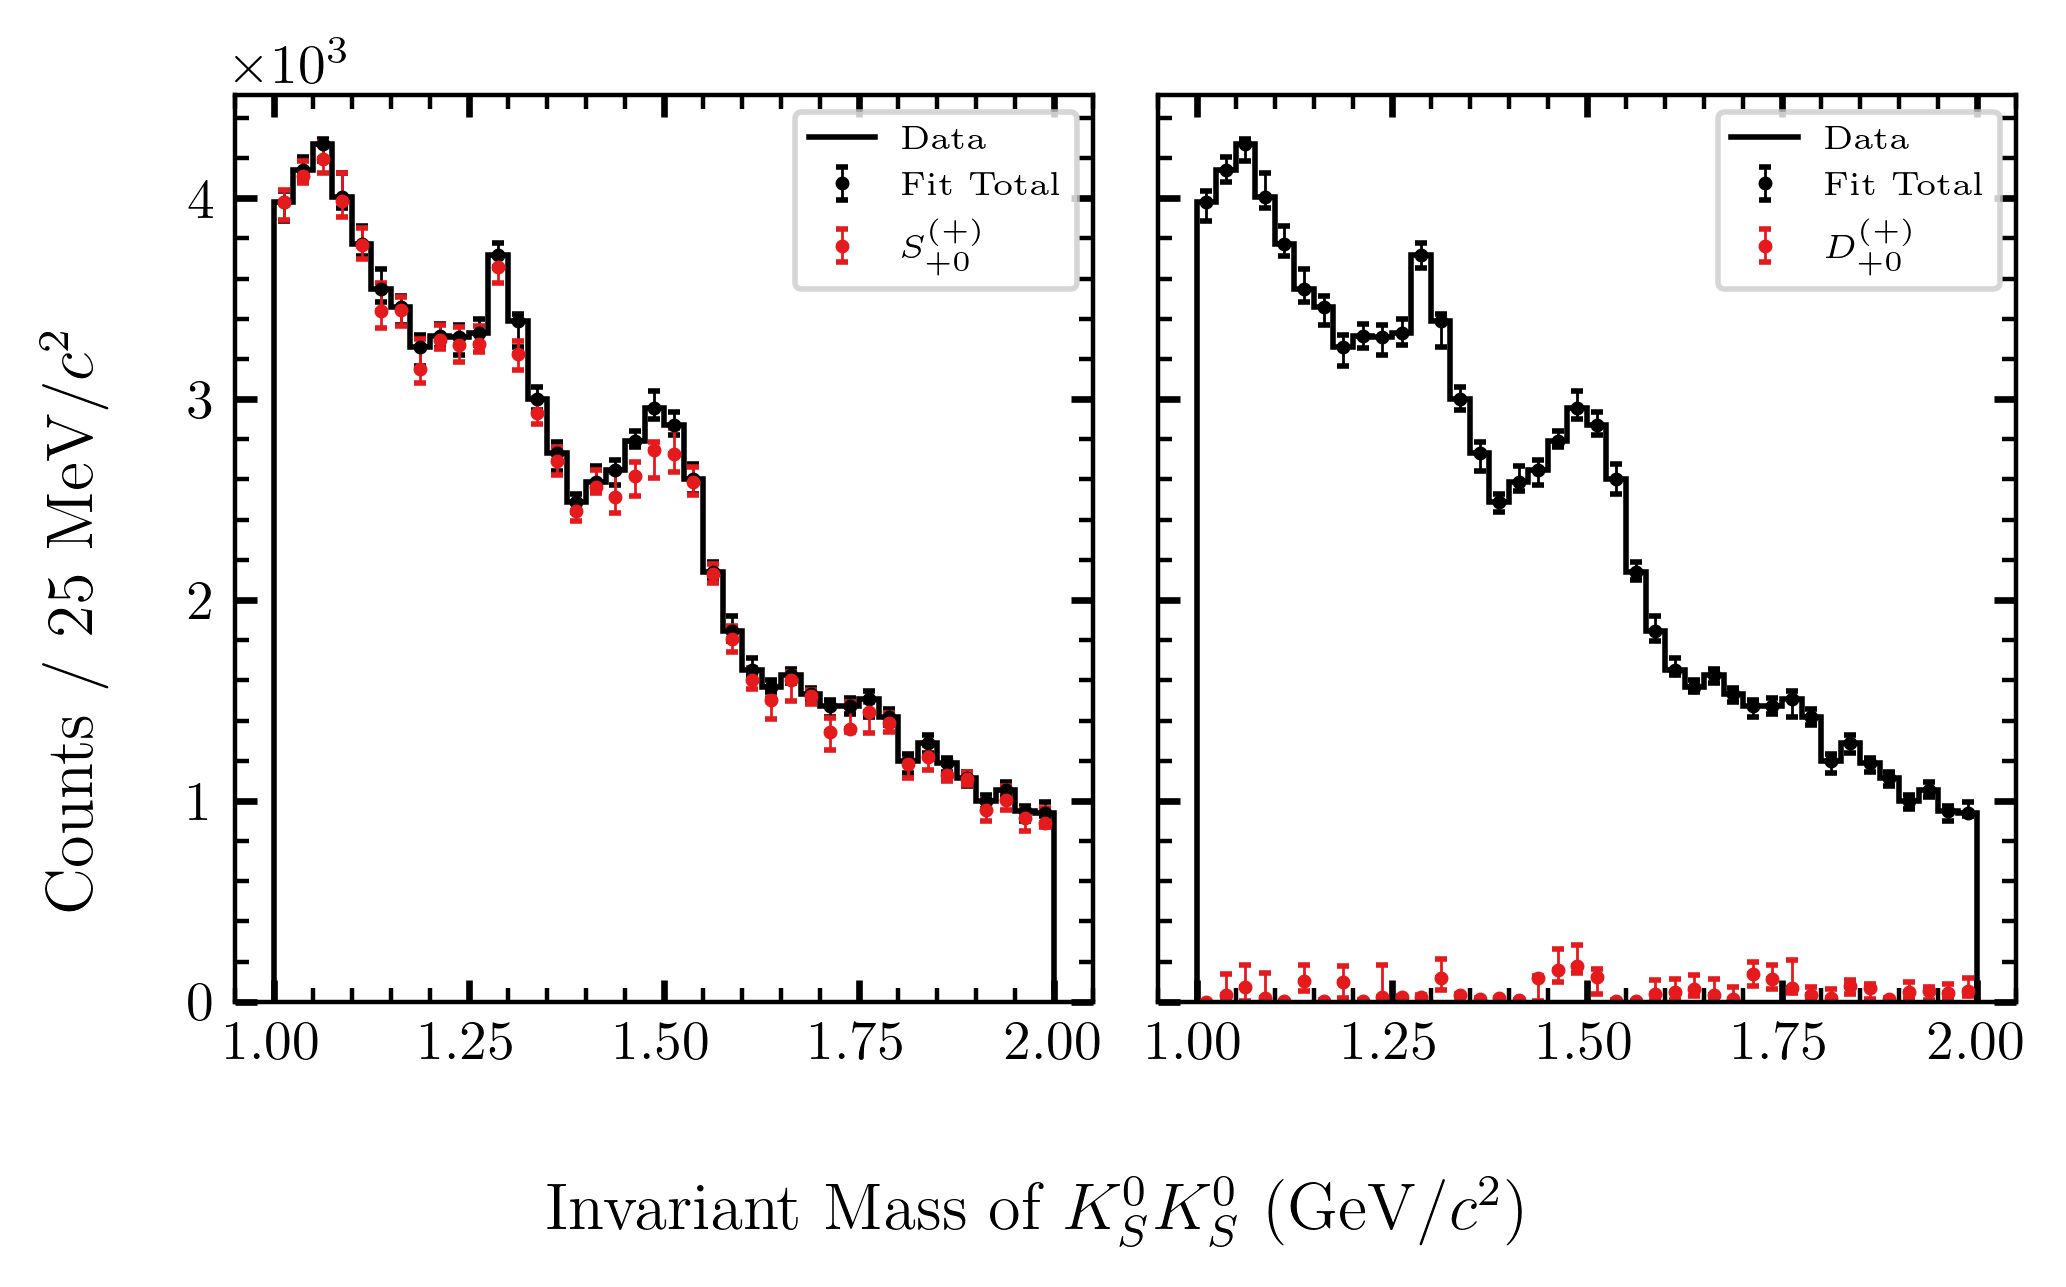
\includegraphics[width=\linewidth]{figures/binned_fit_chisqdof_4.4_splot_D_1s_2b_phase_factor_waves487_uncertainty_bootstrap-CI-BC.png}
        \caption{$\chi^2_\nu < 4.4$}
    \end{subfigure}
    \hfill
    \begin{subfigure}{0.45\textwidth}
        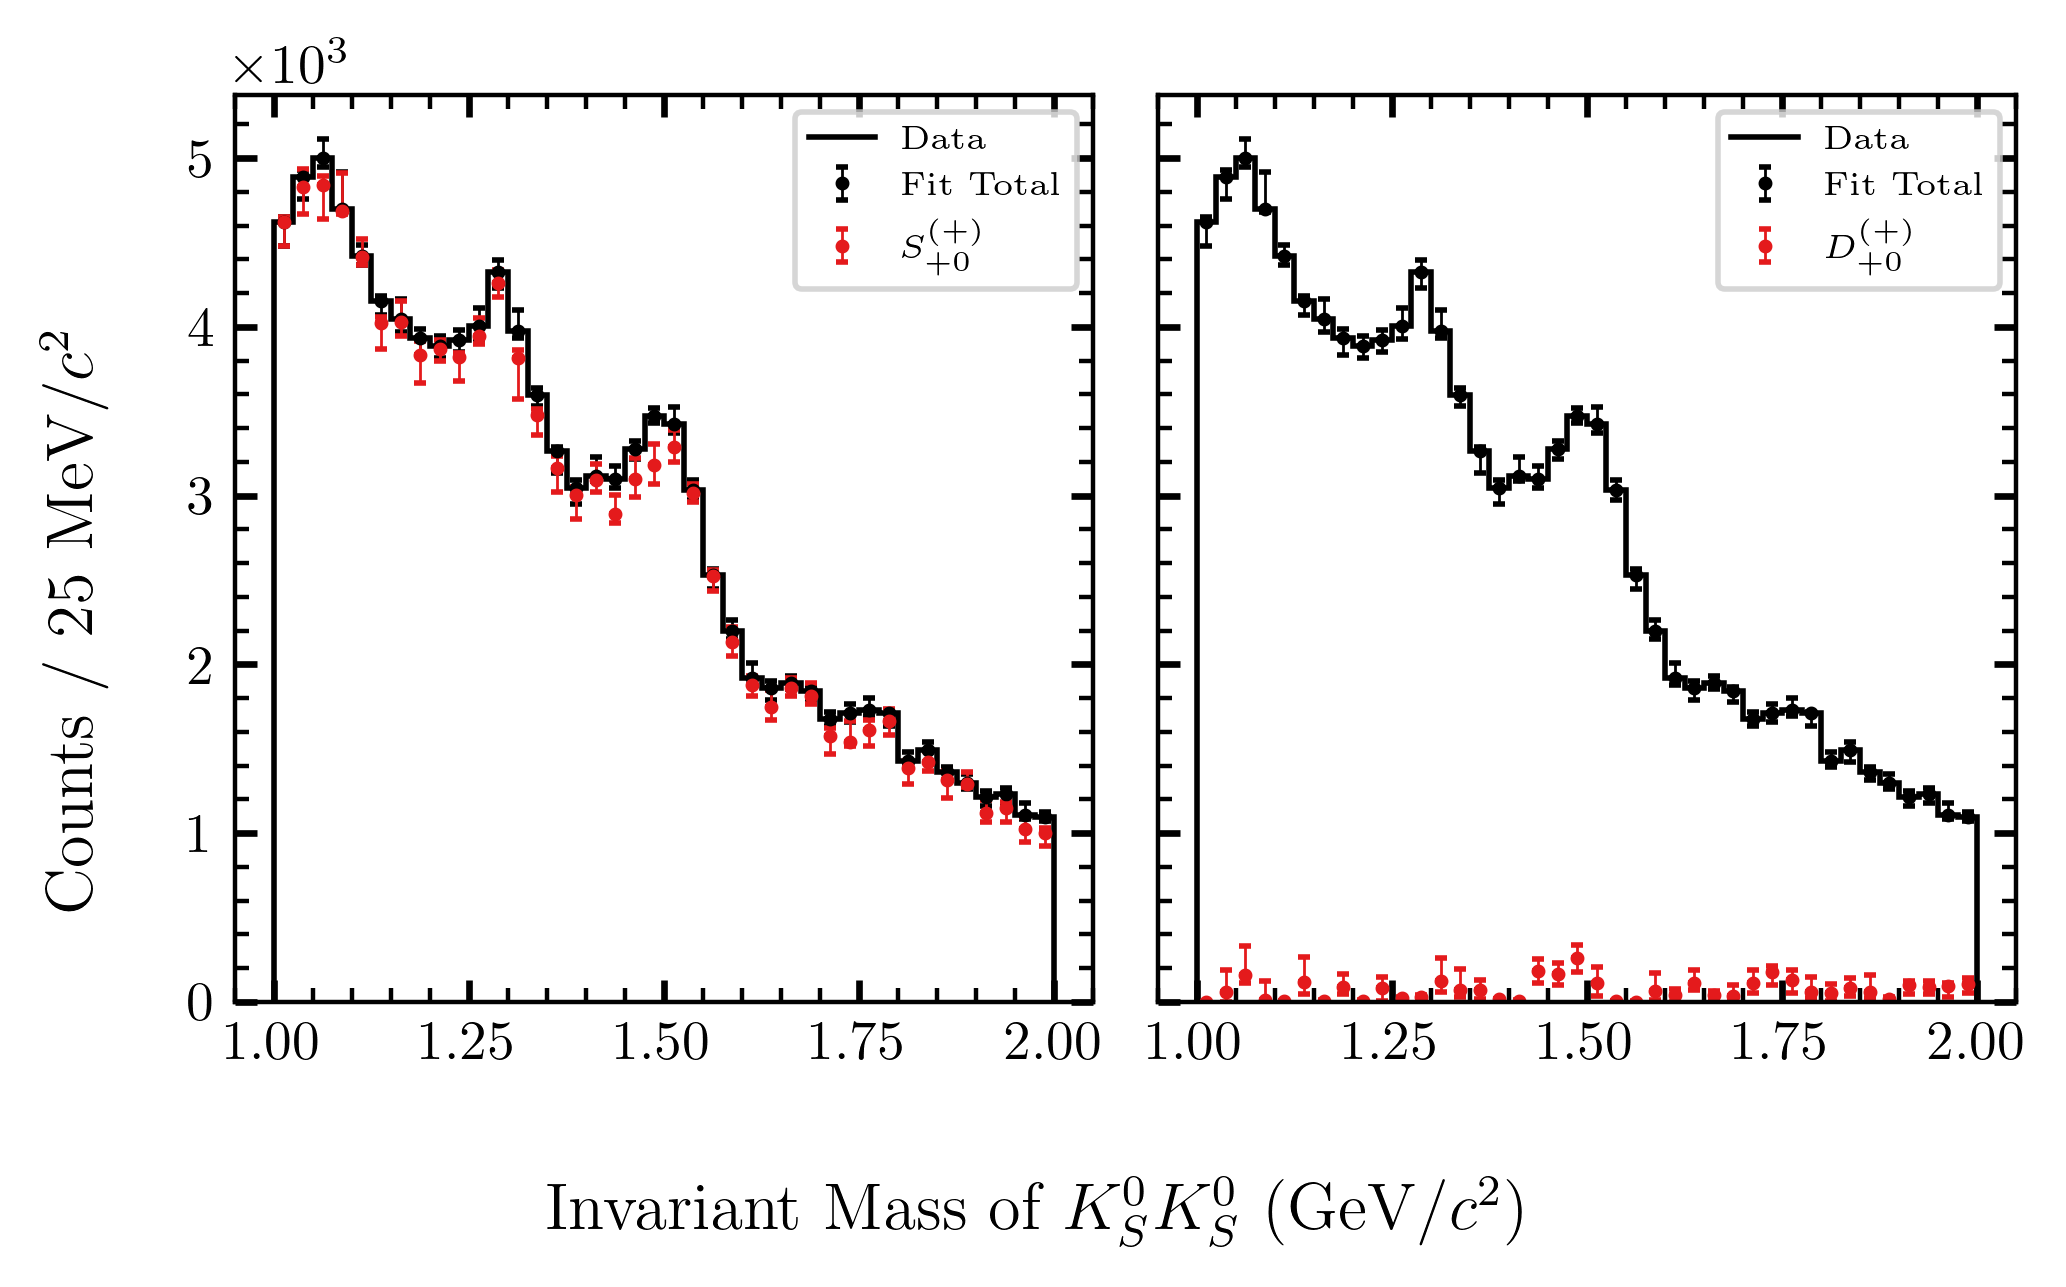
\includegraphics[width=\linewidth]{figures/binned_fit_chisqdof_5.4_splot_D_1s_2b_phase_factor_waves487_uncertainty_bootstrap-CI-BC.png}
        \caption{$\chi^2_\nu < 5.4$}
    \end{subfigure}

    \caption{Binned fit of $S_{0}^{(+)}$, and $D_{0}^{(+)}$ waves. Bars on each fit point correspond to $68\%$ bias-corrected confidence intervals over $ 30 $ bootstrap iterations.}
    \label{fig:binned-fit-all-Sp-D0p}
\end{figure}

\begin{figure}[htbp]
    \centering
    \begin{subfigure}{0.45\textwidth}
        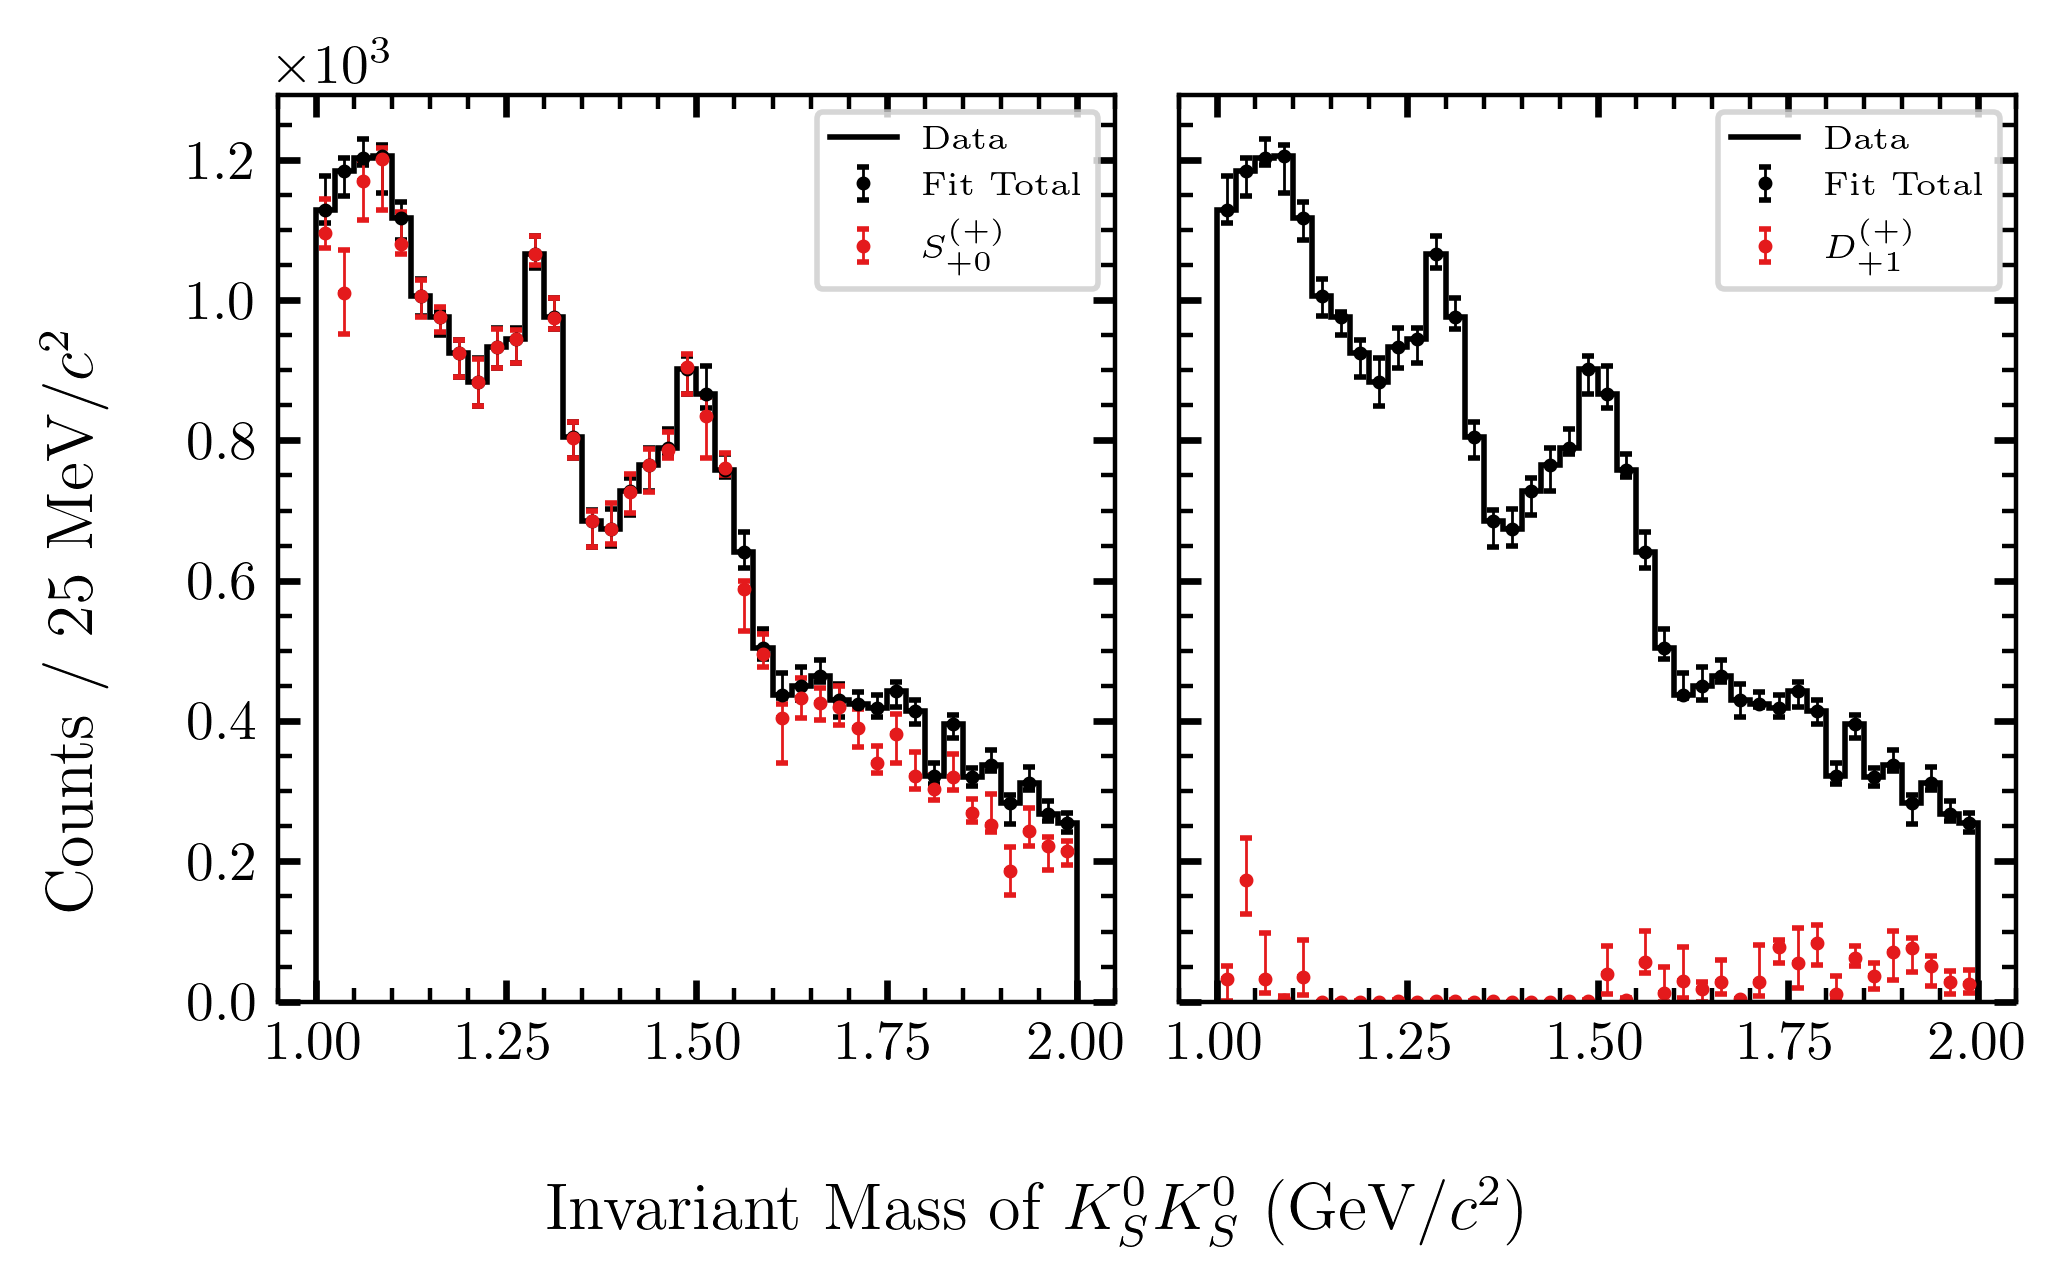
\includegraphics[width=\linewidth]{figures/binned_fit_chisqdof_1.4_splot_D_1s_2b_phase_factor_waves489_uncertainty_bootstrap-CI-BC.png}
        \caption{$\chi^2_\nu < 1.4$}
    \end{subfigure}
    \hfill
    \begin{subfigure}{0.45\textwidth}
        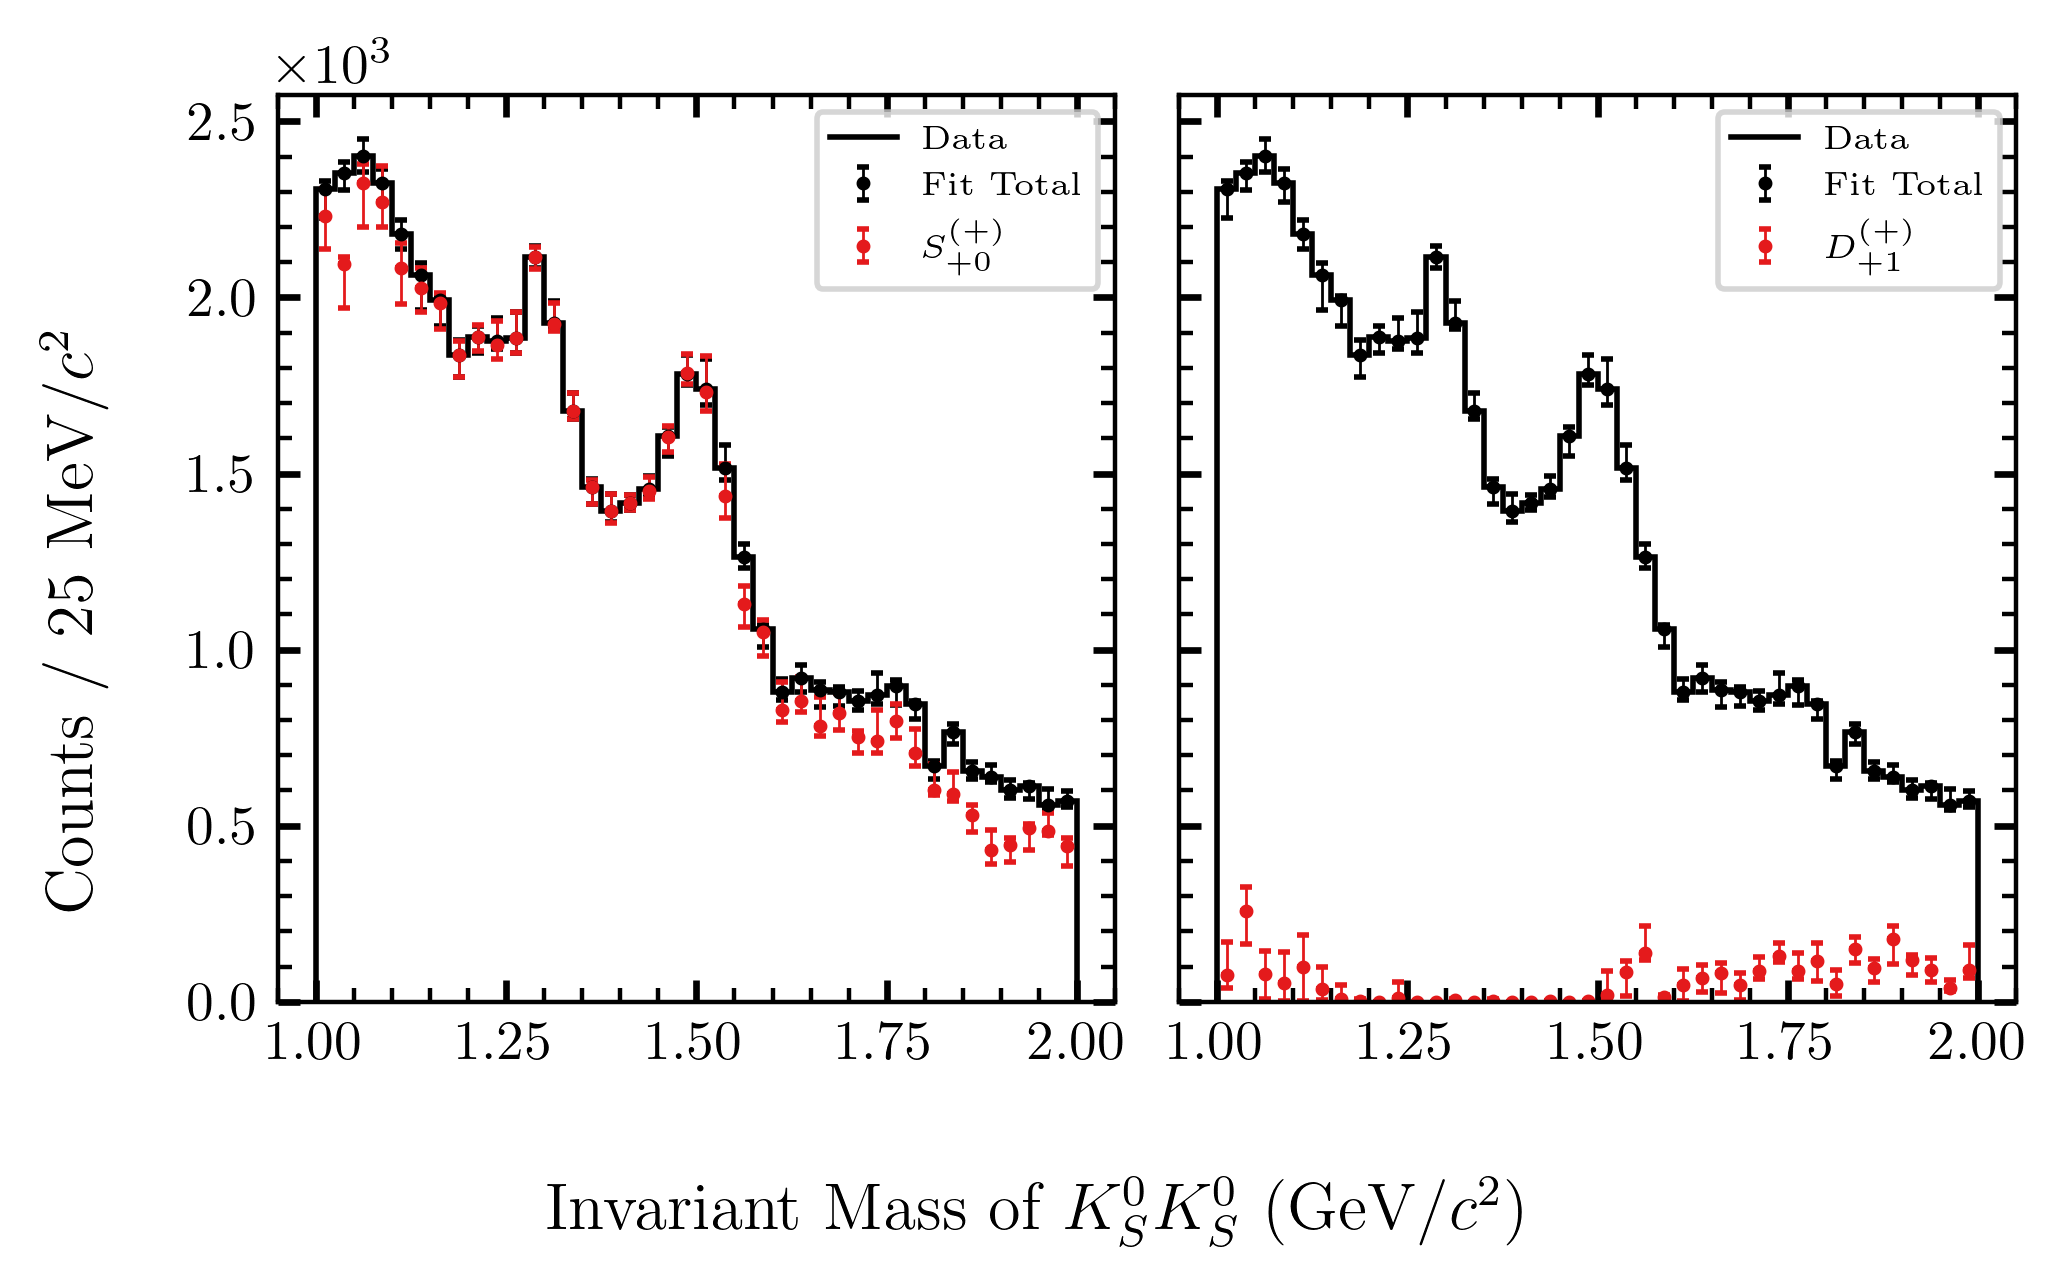
\includegraphics[width=\linewidth]{figures/binned_fit_chisqdof_2.4_splot_D_1s_2b_phase_factor_waves489_uncertainty_bootstrap-CI-BC.png}
        \caption{$\chi^2_\nu < 2.4$}
    \end{subfigure}

    \vspace{1em}

    \begin{subfigure}{0.8\textwidth}
        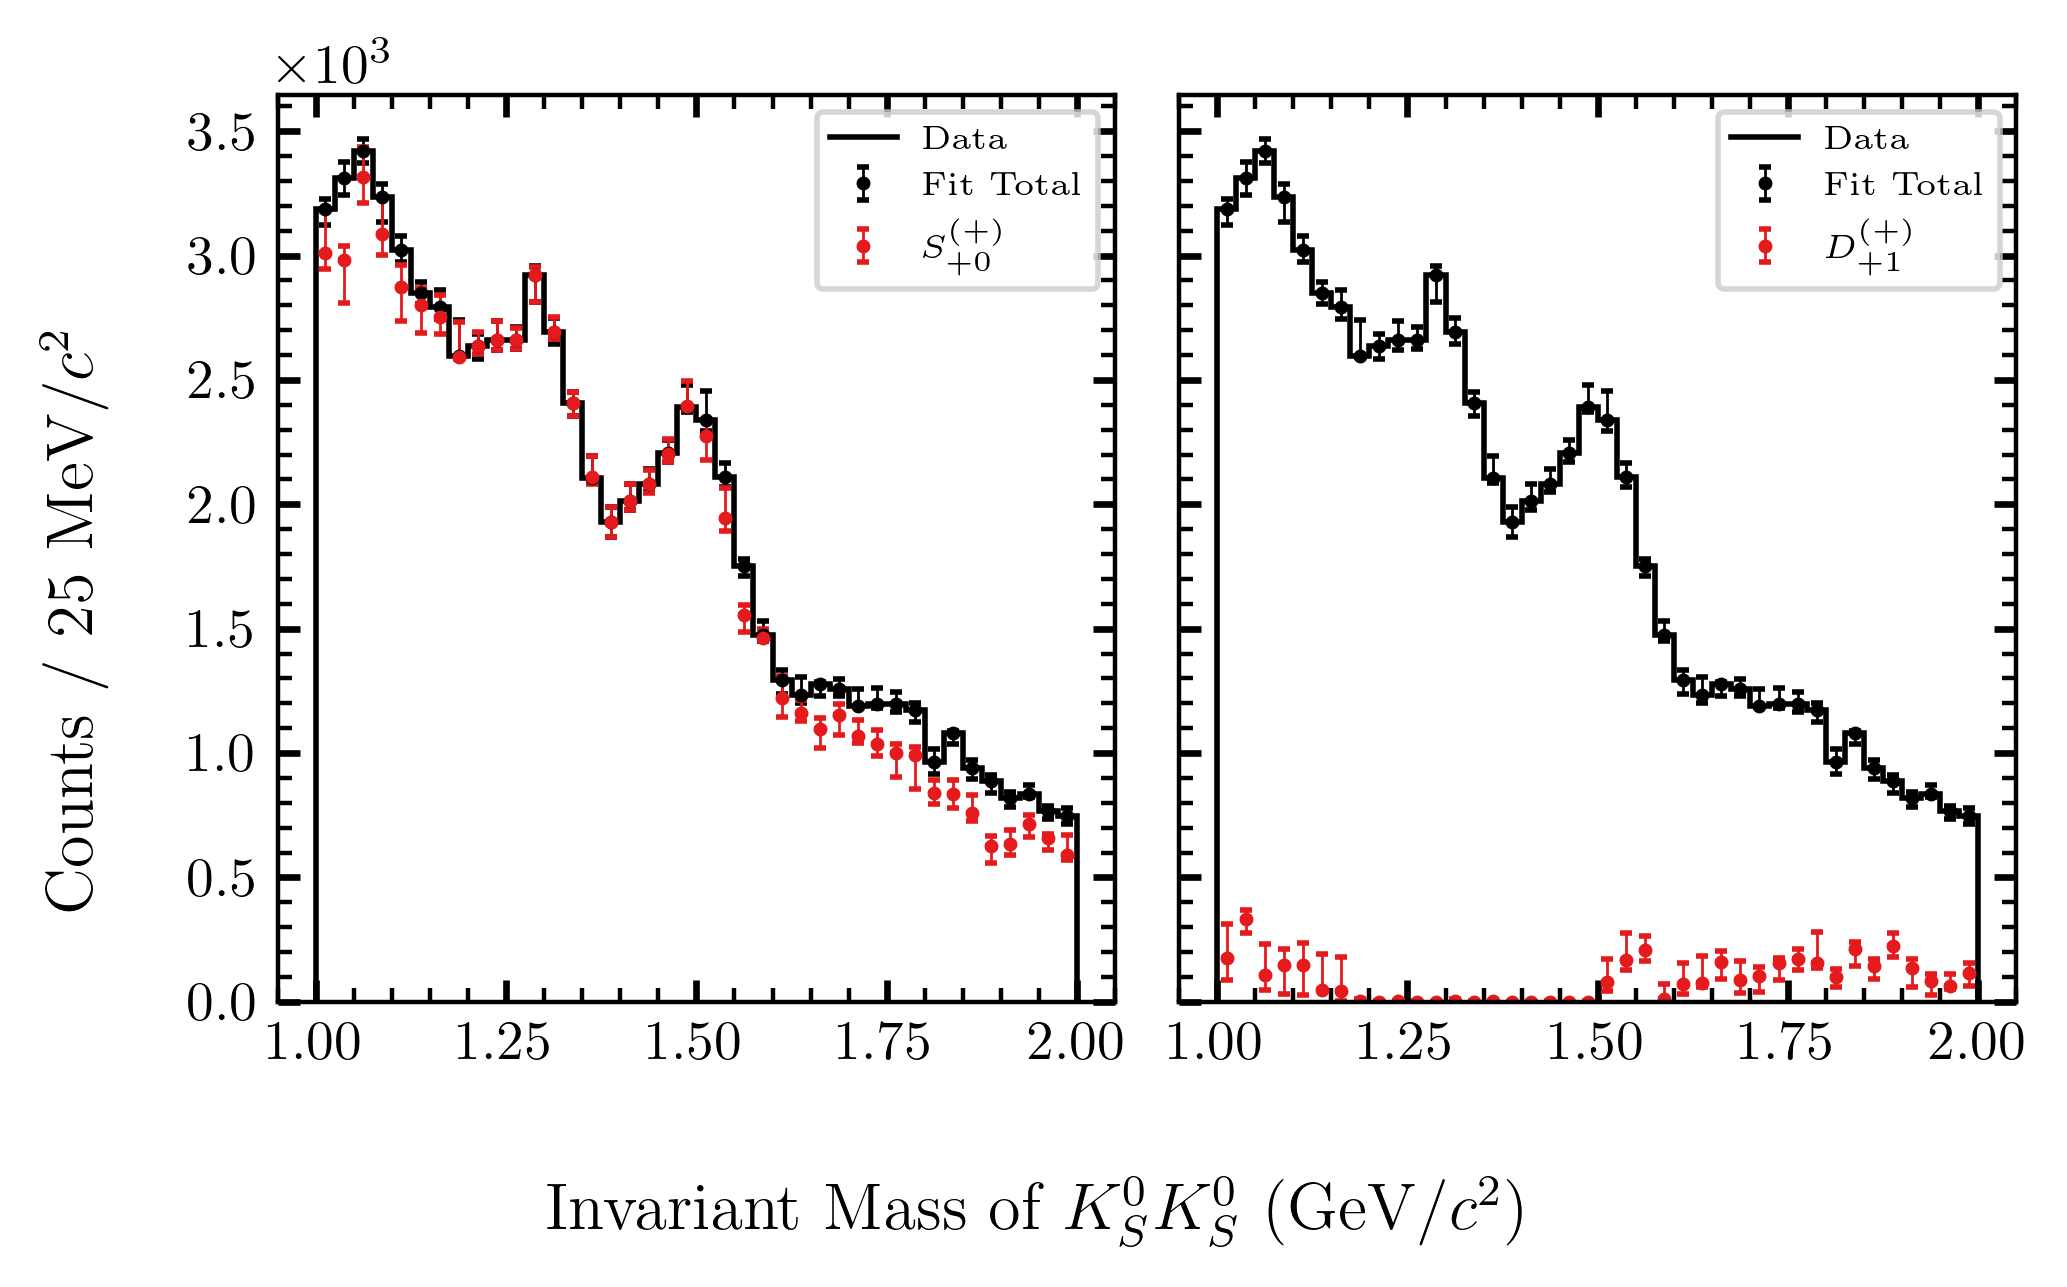
\includegraphics[width=\linewidth]{figures/binned_fit_chisqdof_3.4_splot_D_1s_2b_phase_factor_waves489_uncertainty_bootstrap-CI-BC.png}
        \caption{$\chi^2_\nu < 3.4$}
    \end{subfigure}

    \vspace{1em}

    \begin{subfigure}{0.45\textwidth}
        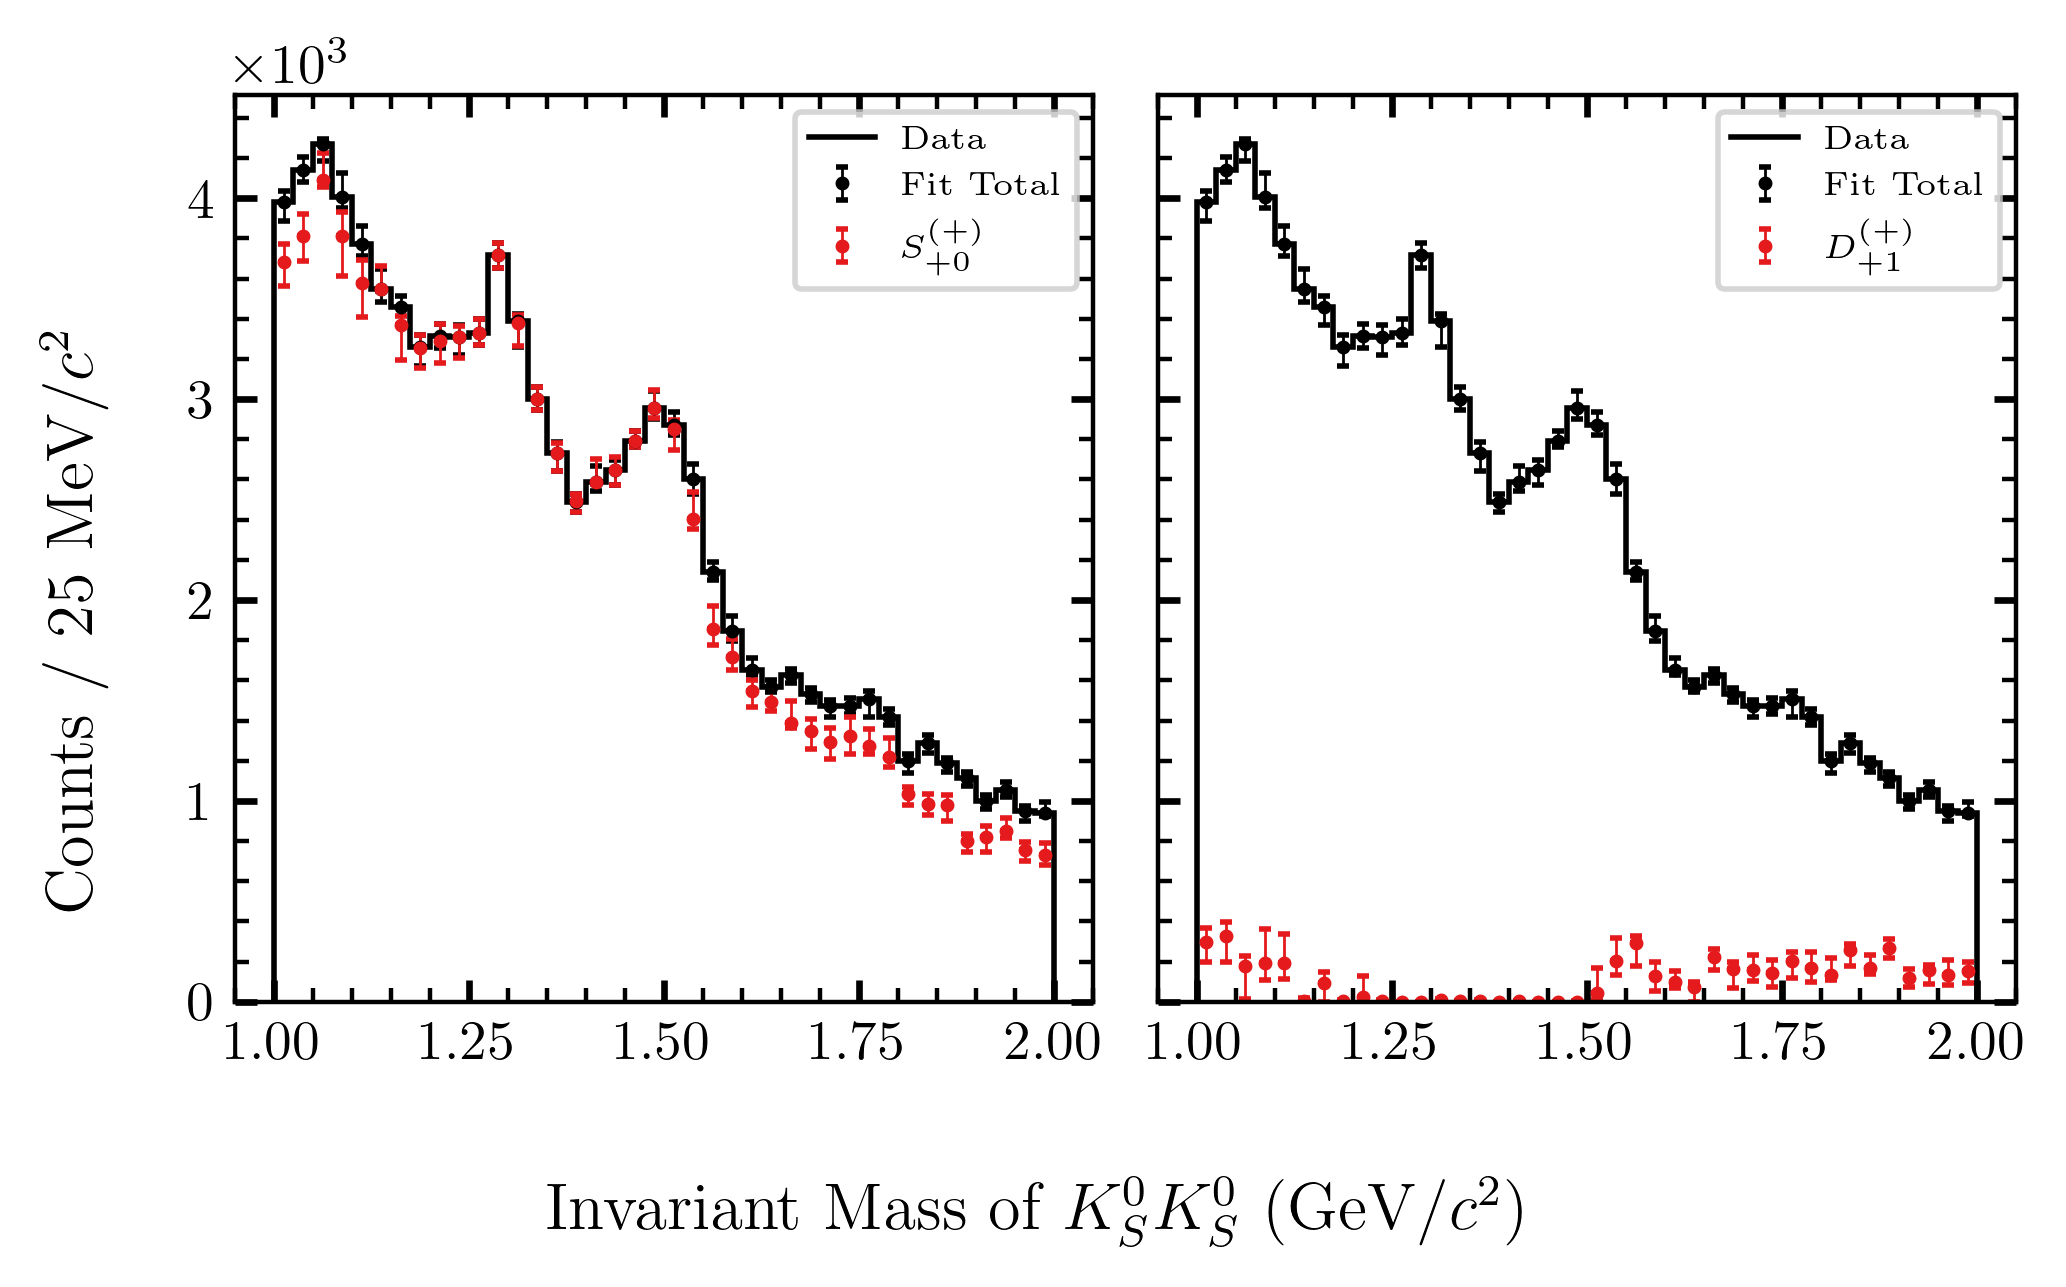
\includegraphics[width=\linewidth]{figures/binned_fit_chisqdof_4.4_splot_D_1s_2b_phase_factor_waves489_uncertainty_bootstrap-CI-BC.png}
        \caption{$\chi^2_\nu < 4.4$}
    \end{subfigure}
    \hfill
    \begin{subfigure}{0.45\textwidth}
        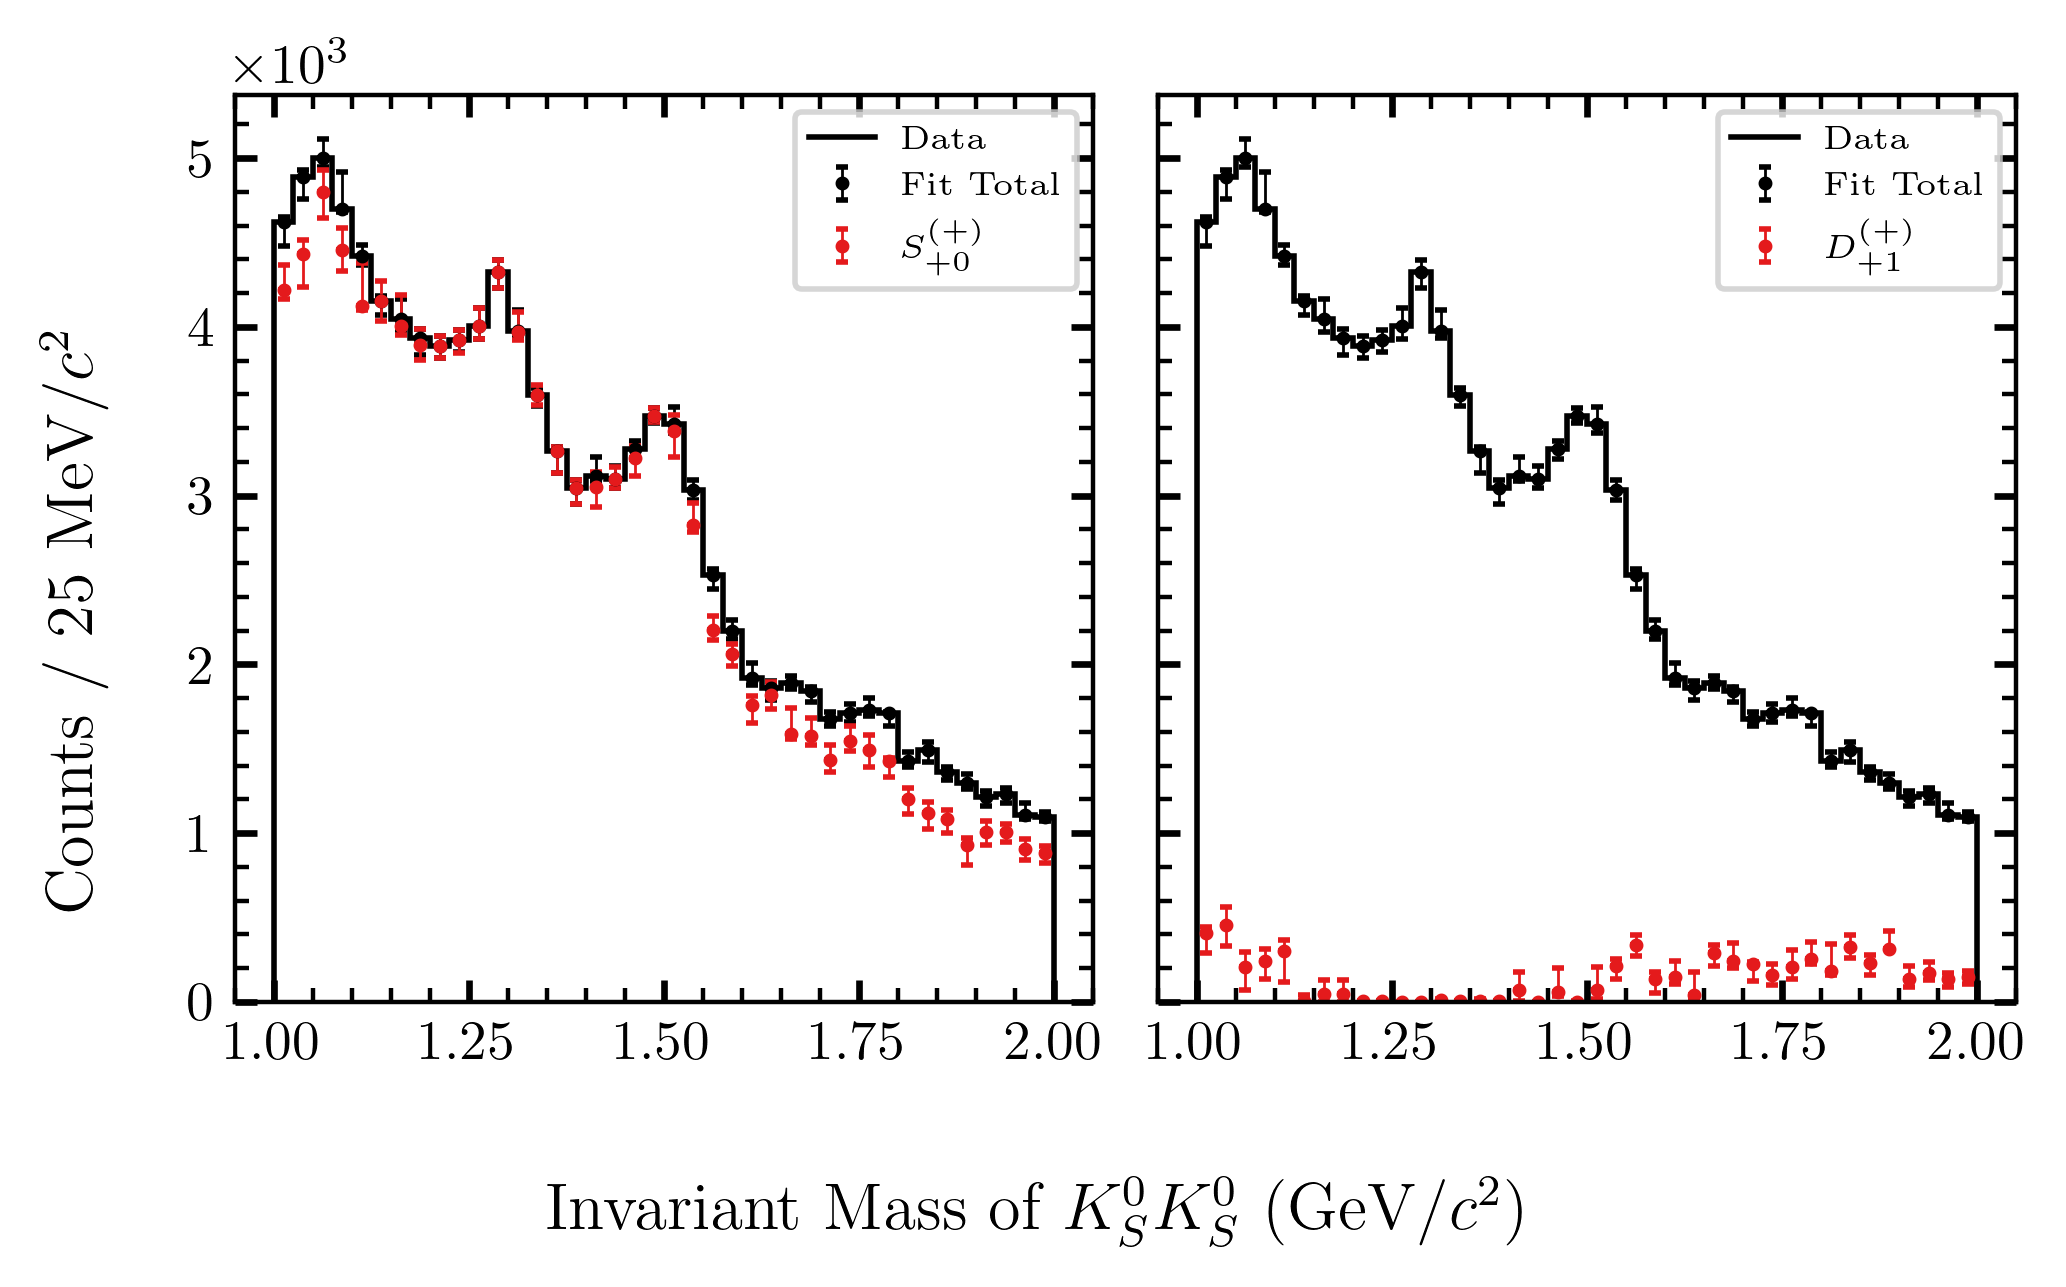
\includegraphics[width=\linewidth]{figures/binned_fit_chisqdof_5.4_splot_D_1s_2b_phase_factor_waves489_uncertainty_bootstrap-CI-BC.png}
        \caption{$\chi^2_\nu < 5.4$}
    \end{subfigure}

    \caption{Binned fit of $S_{0}^{(+)}$, and $D_{1}^{(+)}$ waves. Bars on each fit point correspond to $68\%$ bias-corrected confidence intervals over $ 30 $ bootstrap iterations.}
    \label{fig:binned-fit-all-Sp-D1p}
\end{figure}

\begin{figure}[htbp]
    \centering
    \begin{subfigure}{0.45\textwidth}
        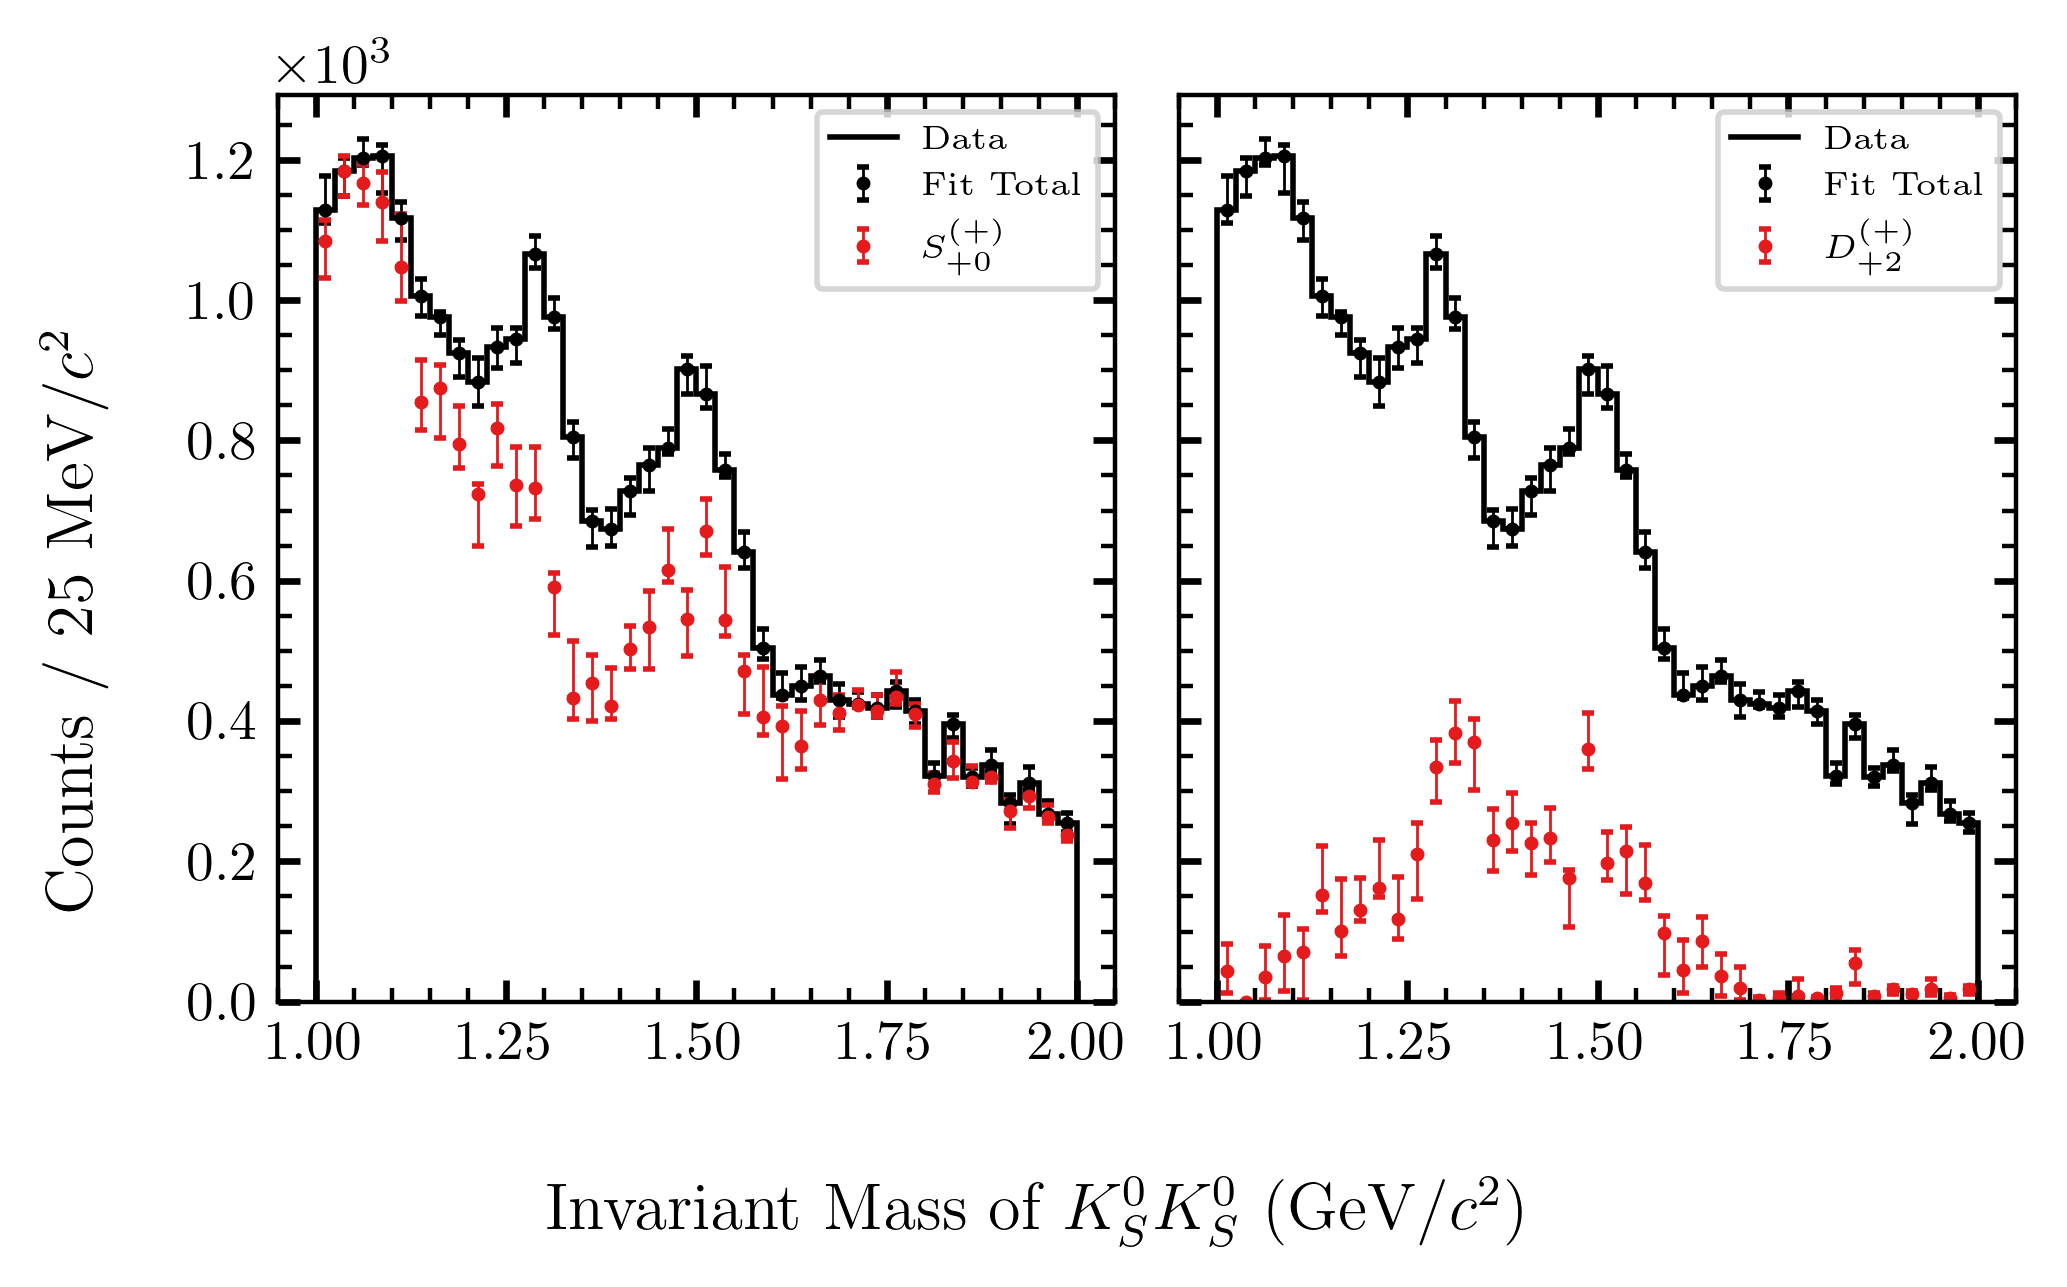
\includegraphics[width=\linewidth]{figures/binned_fit_chisqdof_1.4_splot_D_1s_2b_phase_factor_waves491_uncertainty_bootstrap-CI-BC.png}
        \caption{$\chi^2_\nu < 1.4$}
    \end{subfigure}
    \hfill
    \begin{subfigure}{0.45\textwidth}
        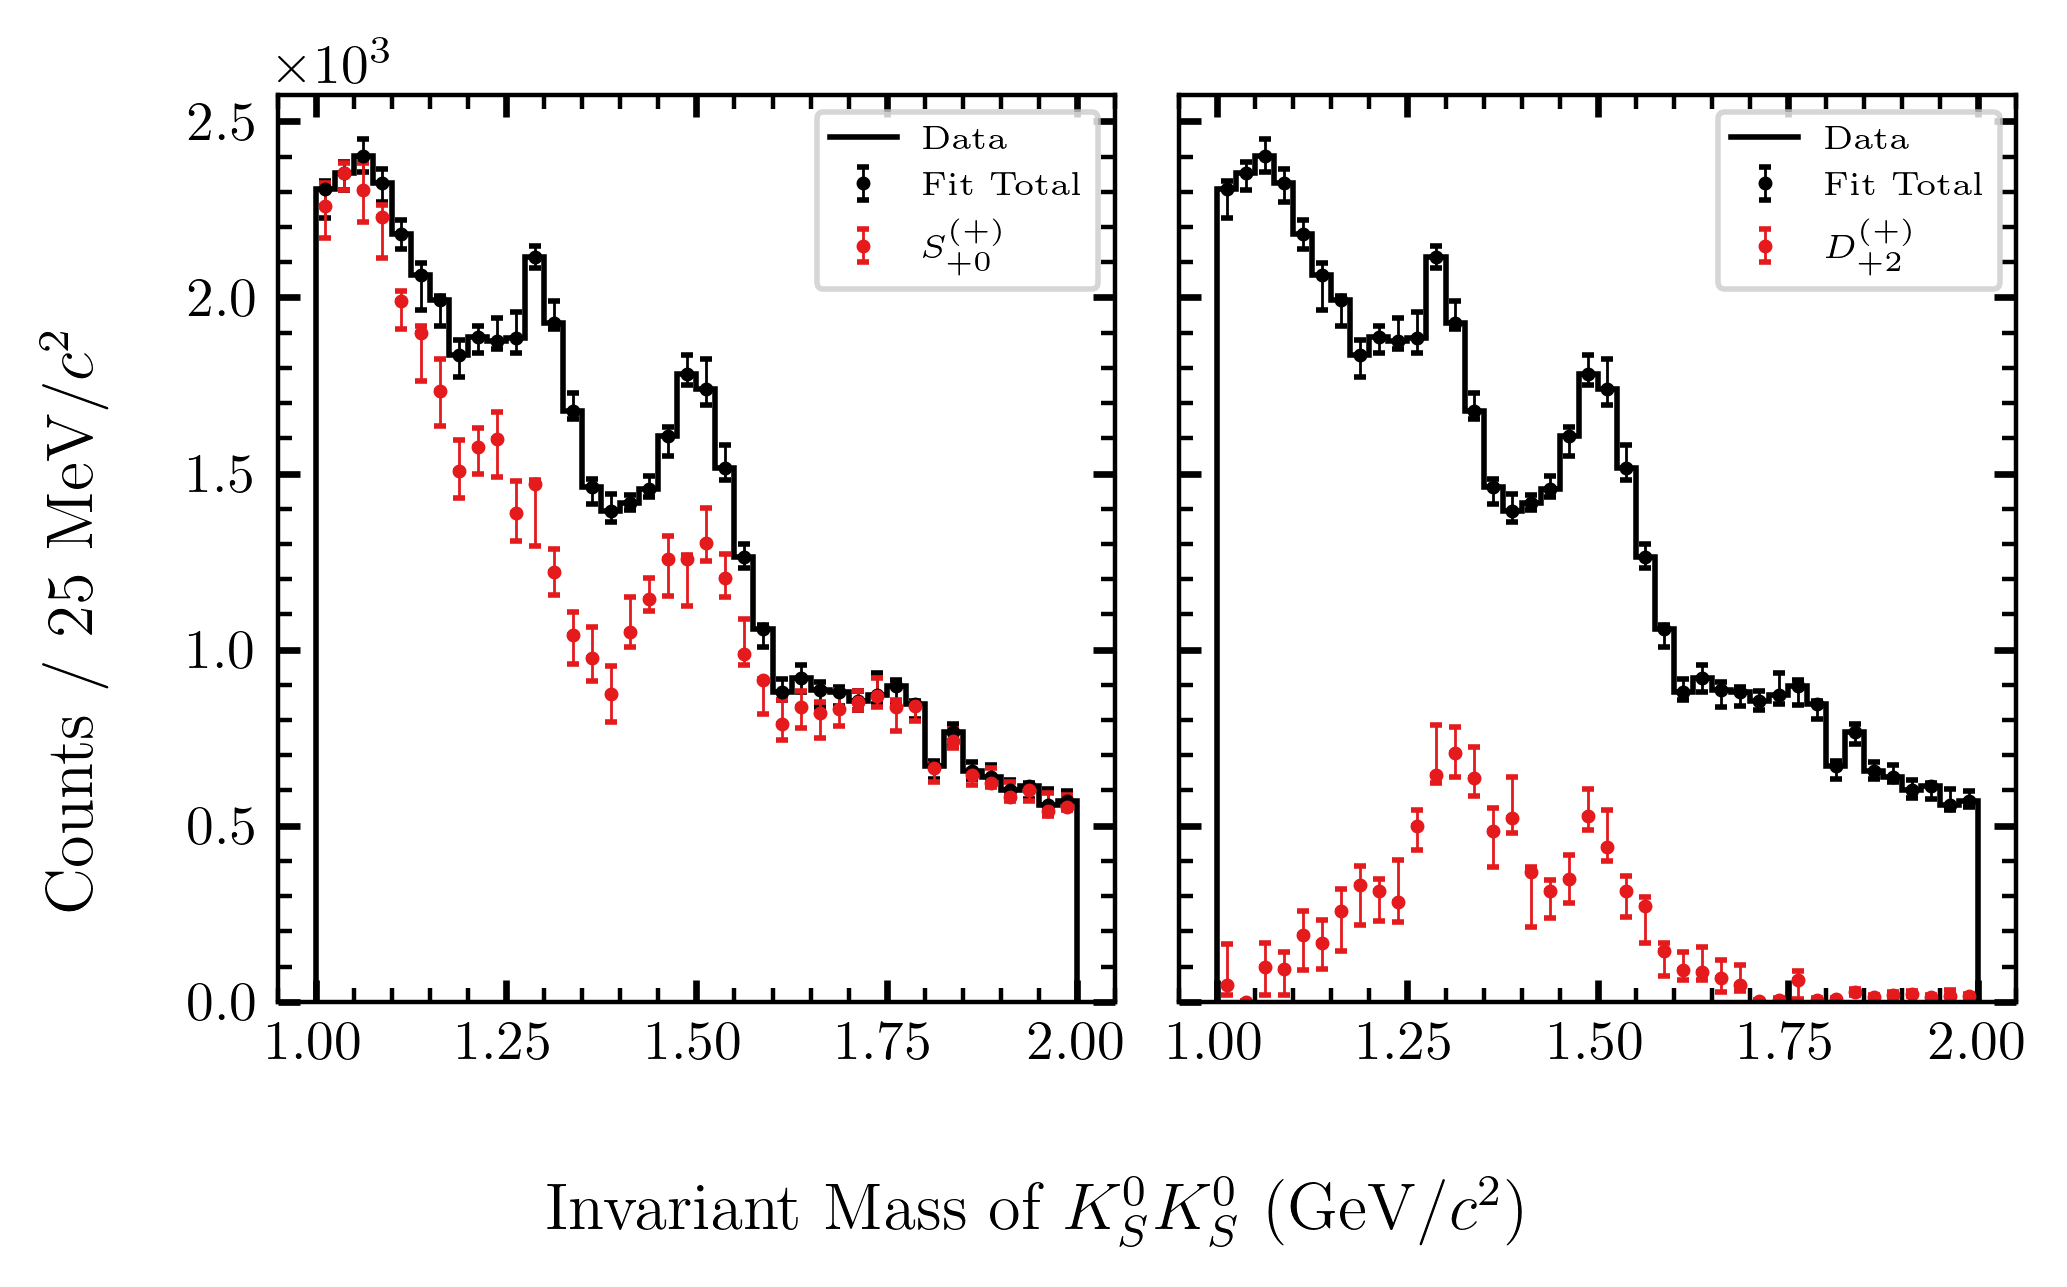
\includegraphics[width=\linewidth]{figures/binned_fit_chisqdof_2.4_splot_D_1s_2b_phase_factor_waves491_uncertainty_bootstrap-CI-BC.png}
        \caption{$\chi^2_\nu < 2.4$}
    \end{subfigure}

    \vspace{1em}

    \begin{subfigure}{0.8\textwidth}
        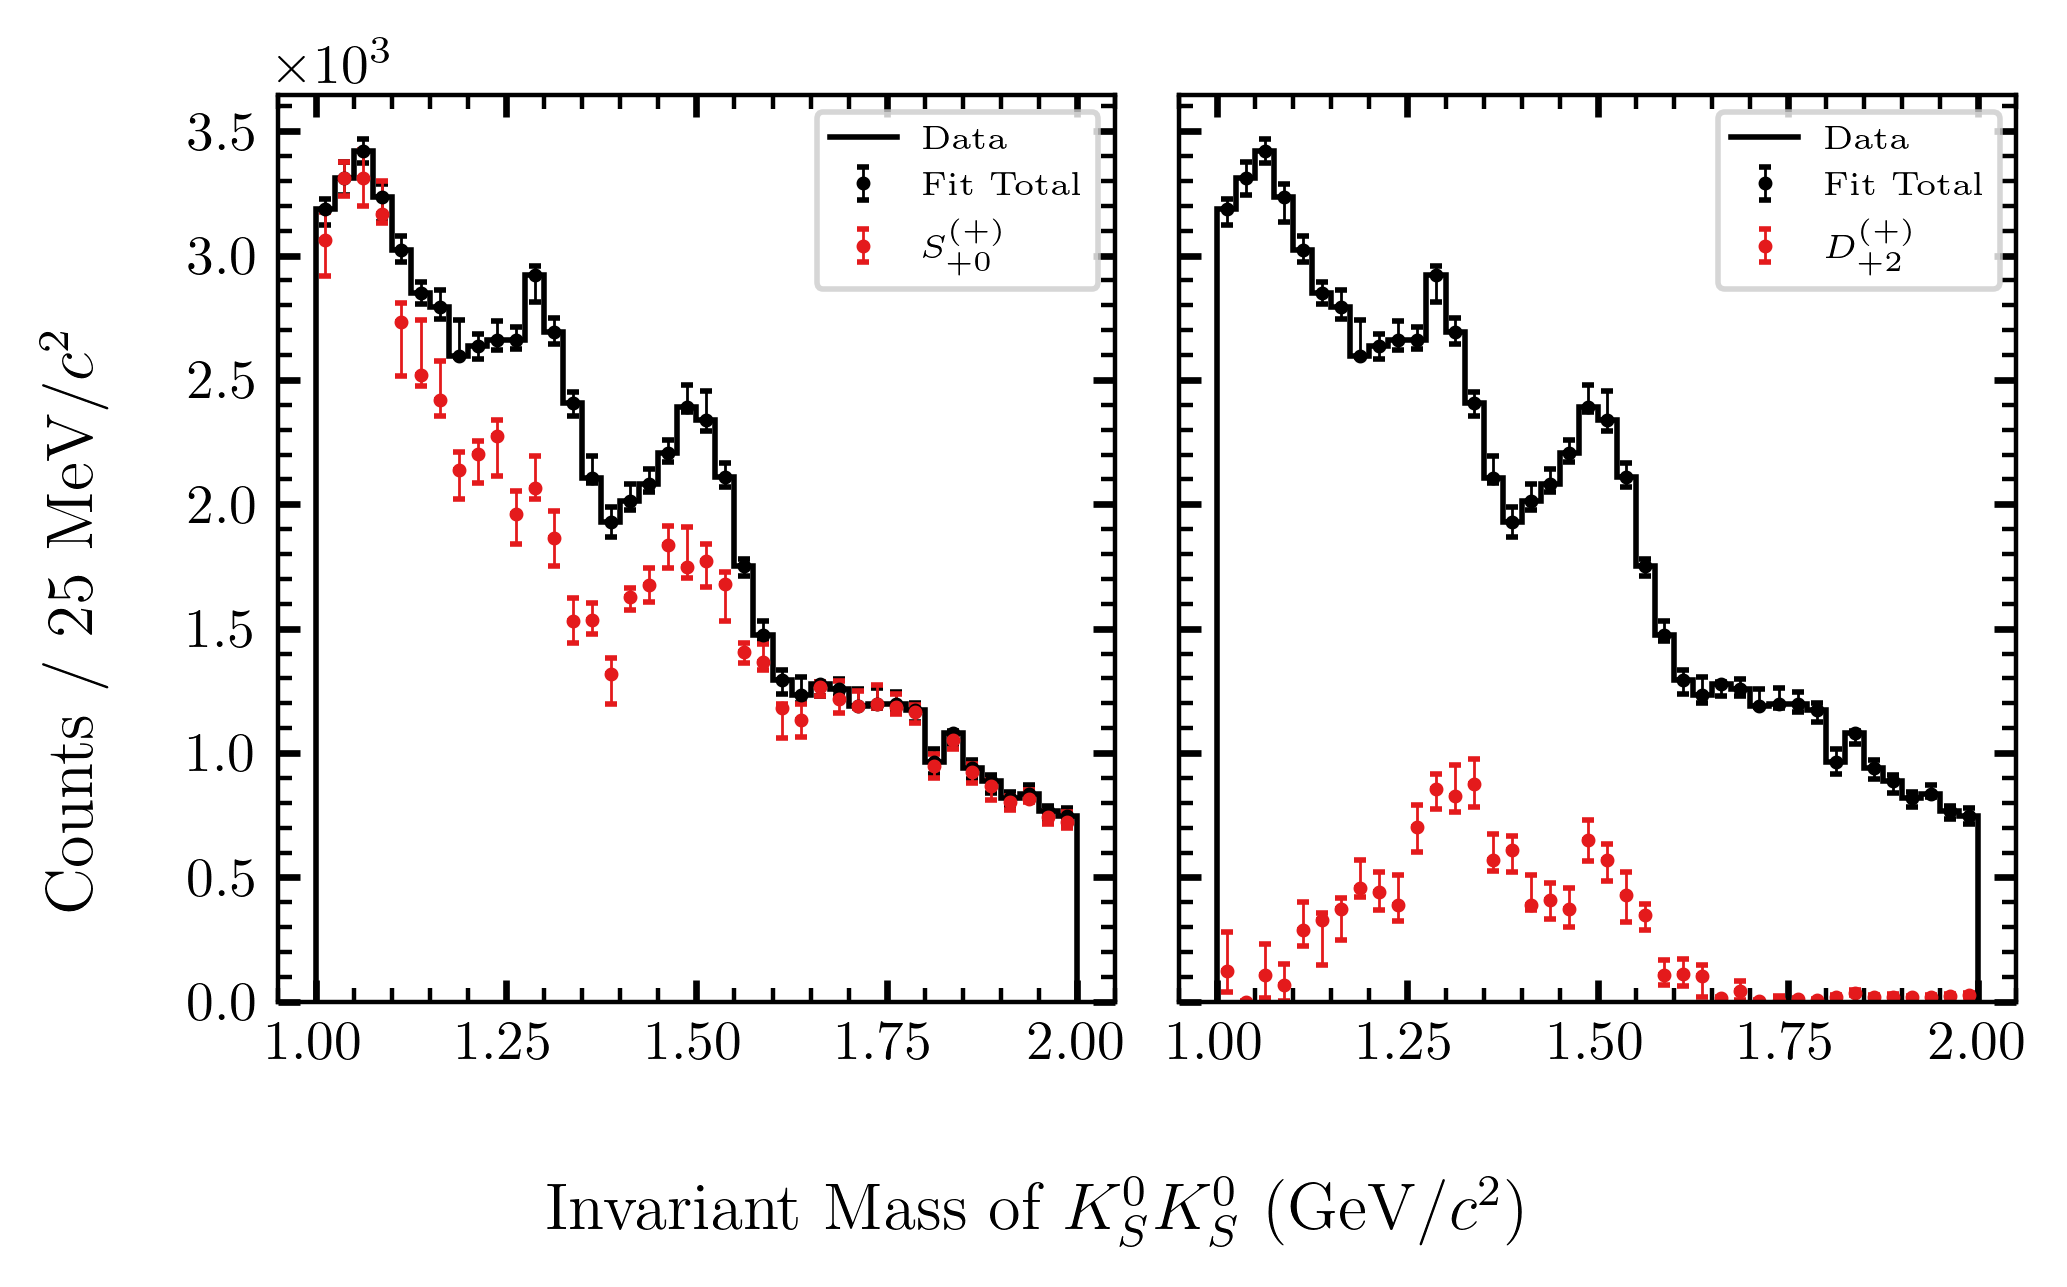
\includegraphics[width=\linewidth]{figures/binned_fit_chisqdof_3.4_splot_D_1s_2b_phase_factor_waves491_uncertainty_bootstrap-CI-BC.png}
        \caption{$\chi^2_\nu < 3.4$}
    \end{subfigure}

    \vspace{1em}

    \begin{subfigure}{0.45\textwidth}
        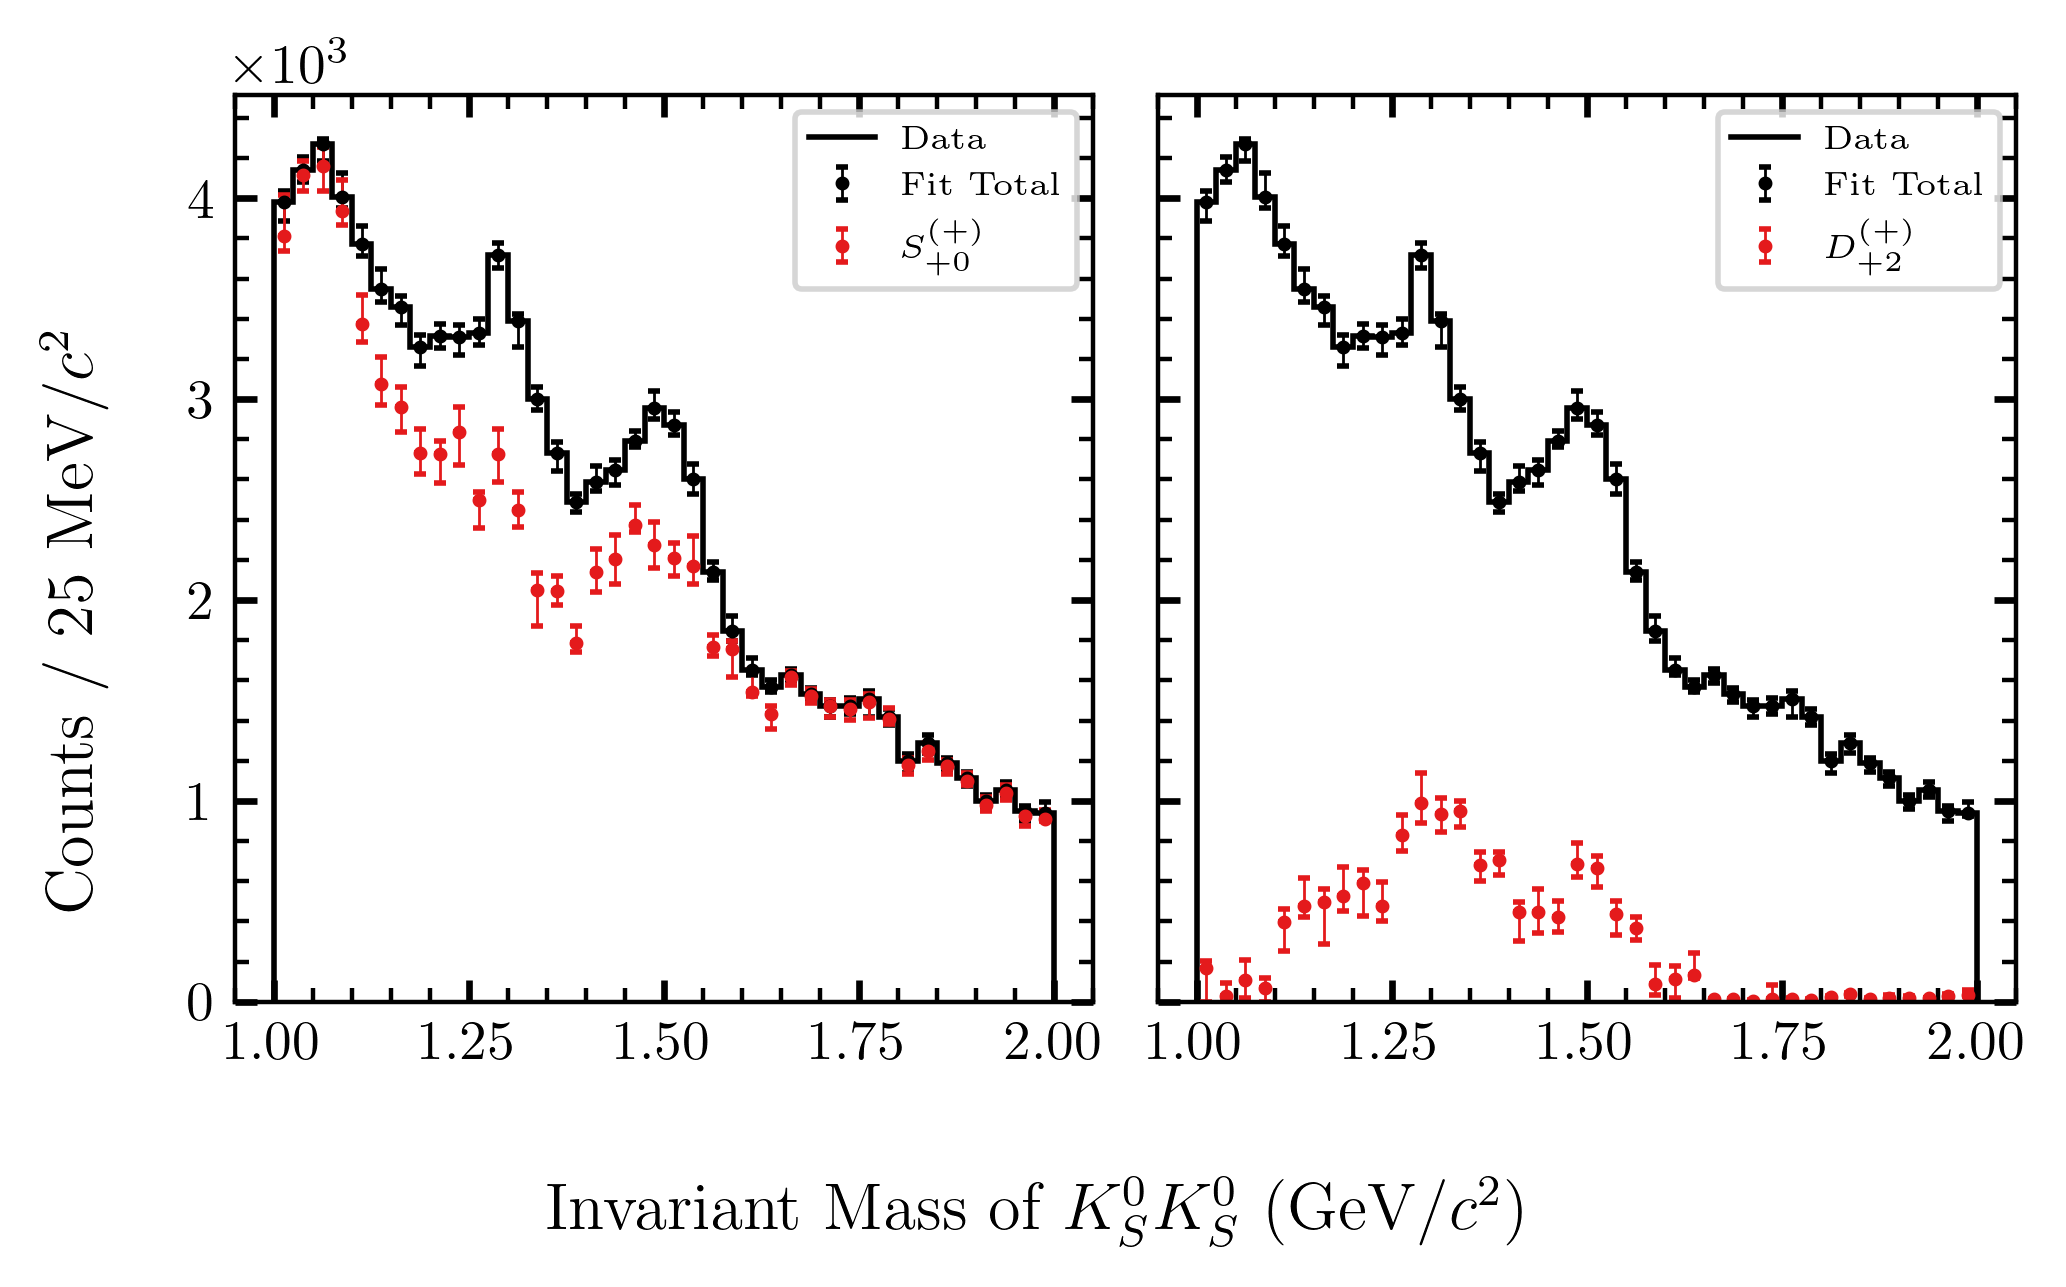
\includegraphics[width=\linewidth]{figures/binned_fit_chisqdof_4.4_splot_D_1s_2b_phase_factor_waves491_uncertainty_bootstrap-CI-BC.png}
        \caption{$\chi^2_\nu < 4.4$}
    \end{subfigure}
    \hfill
    \begin{subfigure}{0.45\textwidth}
        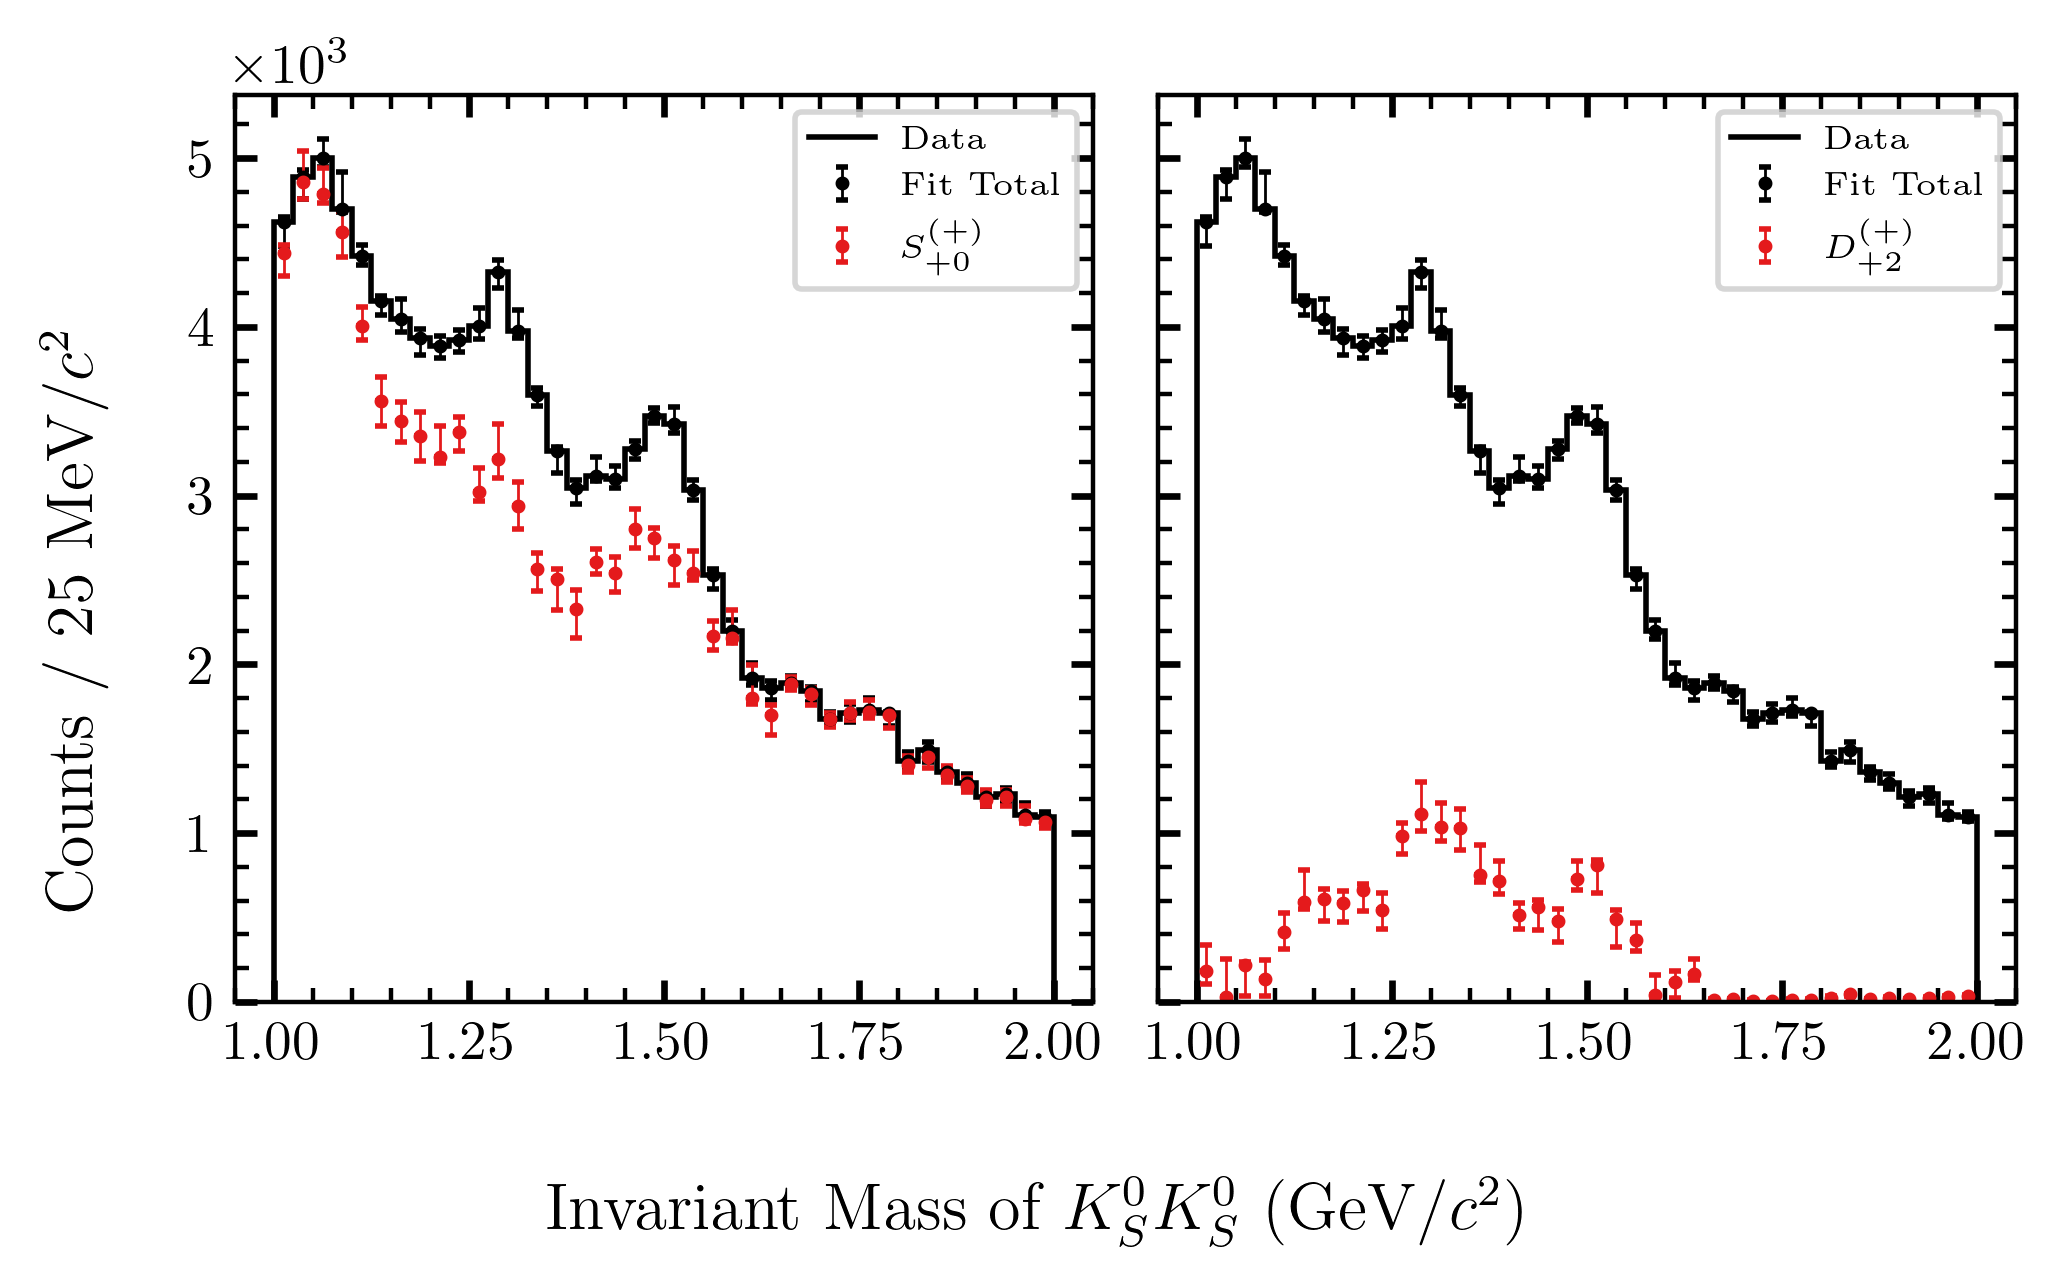
\includegraphics[width=\linewidth]{figures/binned_fit_chisqdof_5.4_splot_D_1s_2b_phase_factor_waves491_uncertainty_bootstrap-CI-BC.png}
        \caption{$\chi^2_\nu < 5.4$}
    \end{subfigure}

    \caption{Binned fit of $S_{0}^{(+)}$, and $D_{+2}^{(+)}$ waves. Bars on each fit point correspond to $68\%$ bias-corrected confidence intervals over $ 30 $ bootstrap iterations.}
    \label{fig:binned-fit-all-Sp-D2p}
\end{figure}

\begin{figure}[htbp]
    \centering
    \begin{subfigure}{0.45\textwidth}
        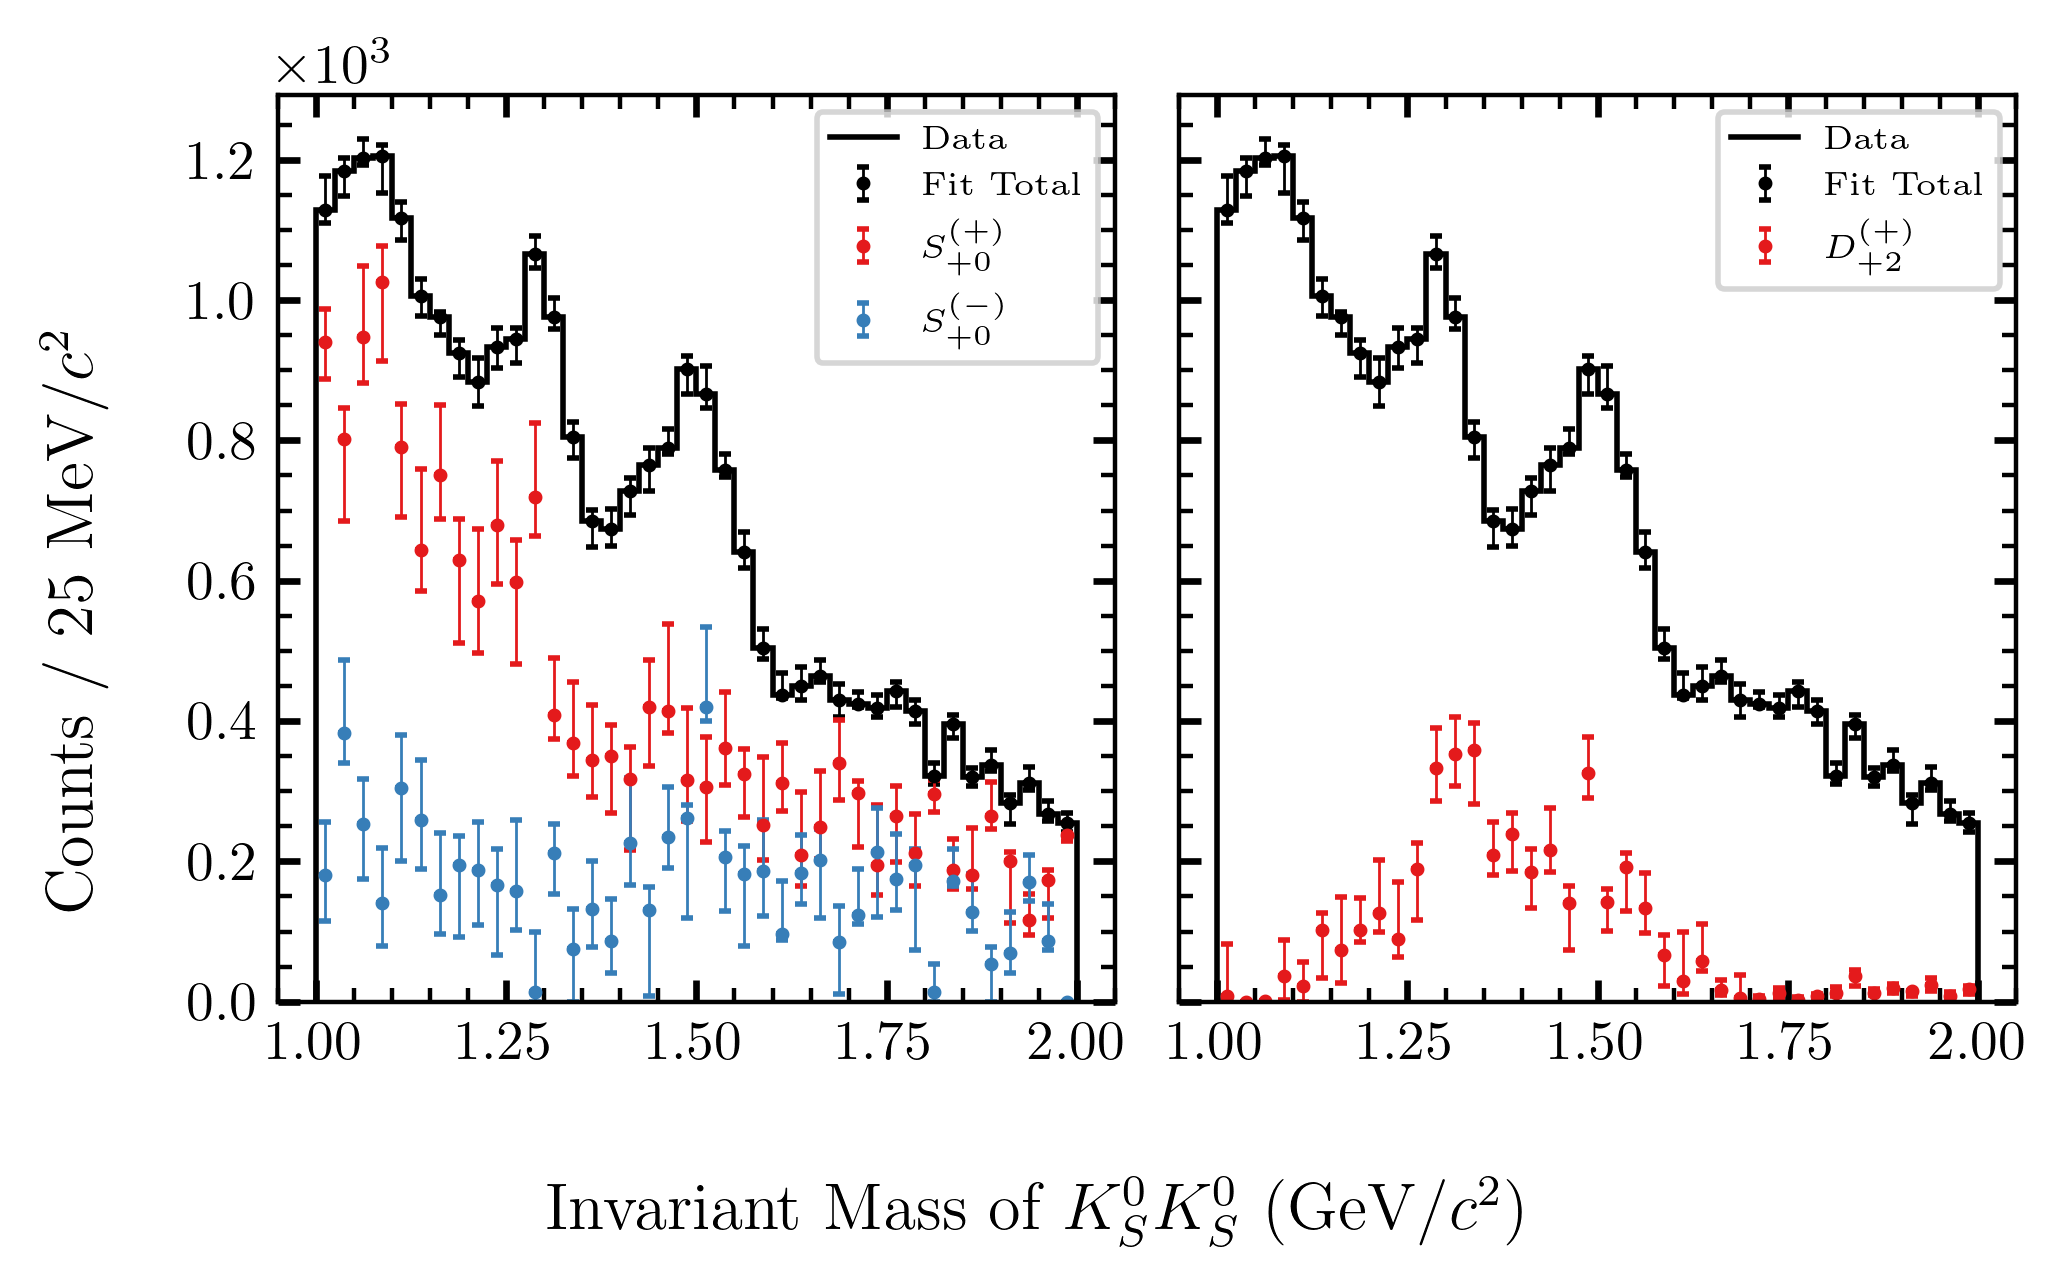
\includegraphics[width=\linewidth]{figures/binned_fit_chisqdof_1.4_splot_D_1s_2b_phase_factor_waves29099_uncertainty_bootstrap-CI-BC.png}
        \caption{$\chi^2_\nu < 1.4$}
    \end{subfigure}
    \hfill
    \begin{subfigure}{0.45\textwidth}
        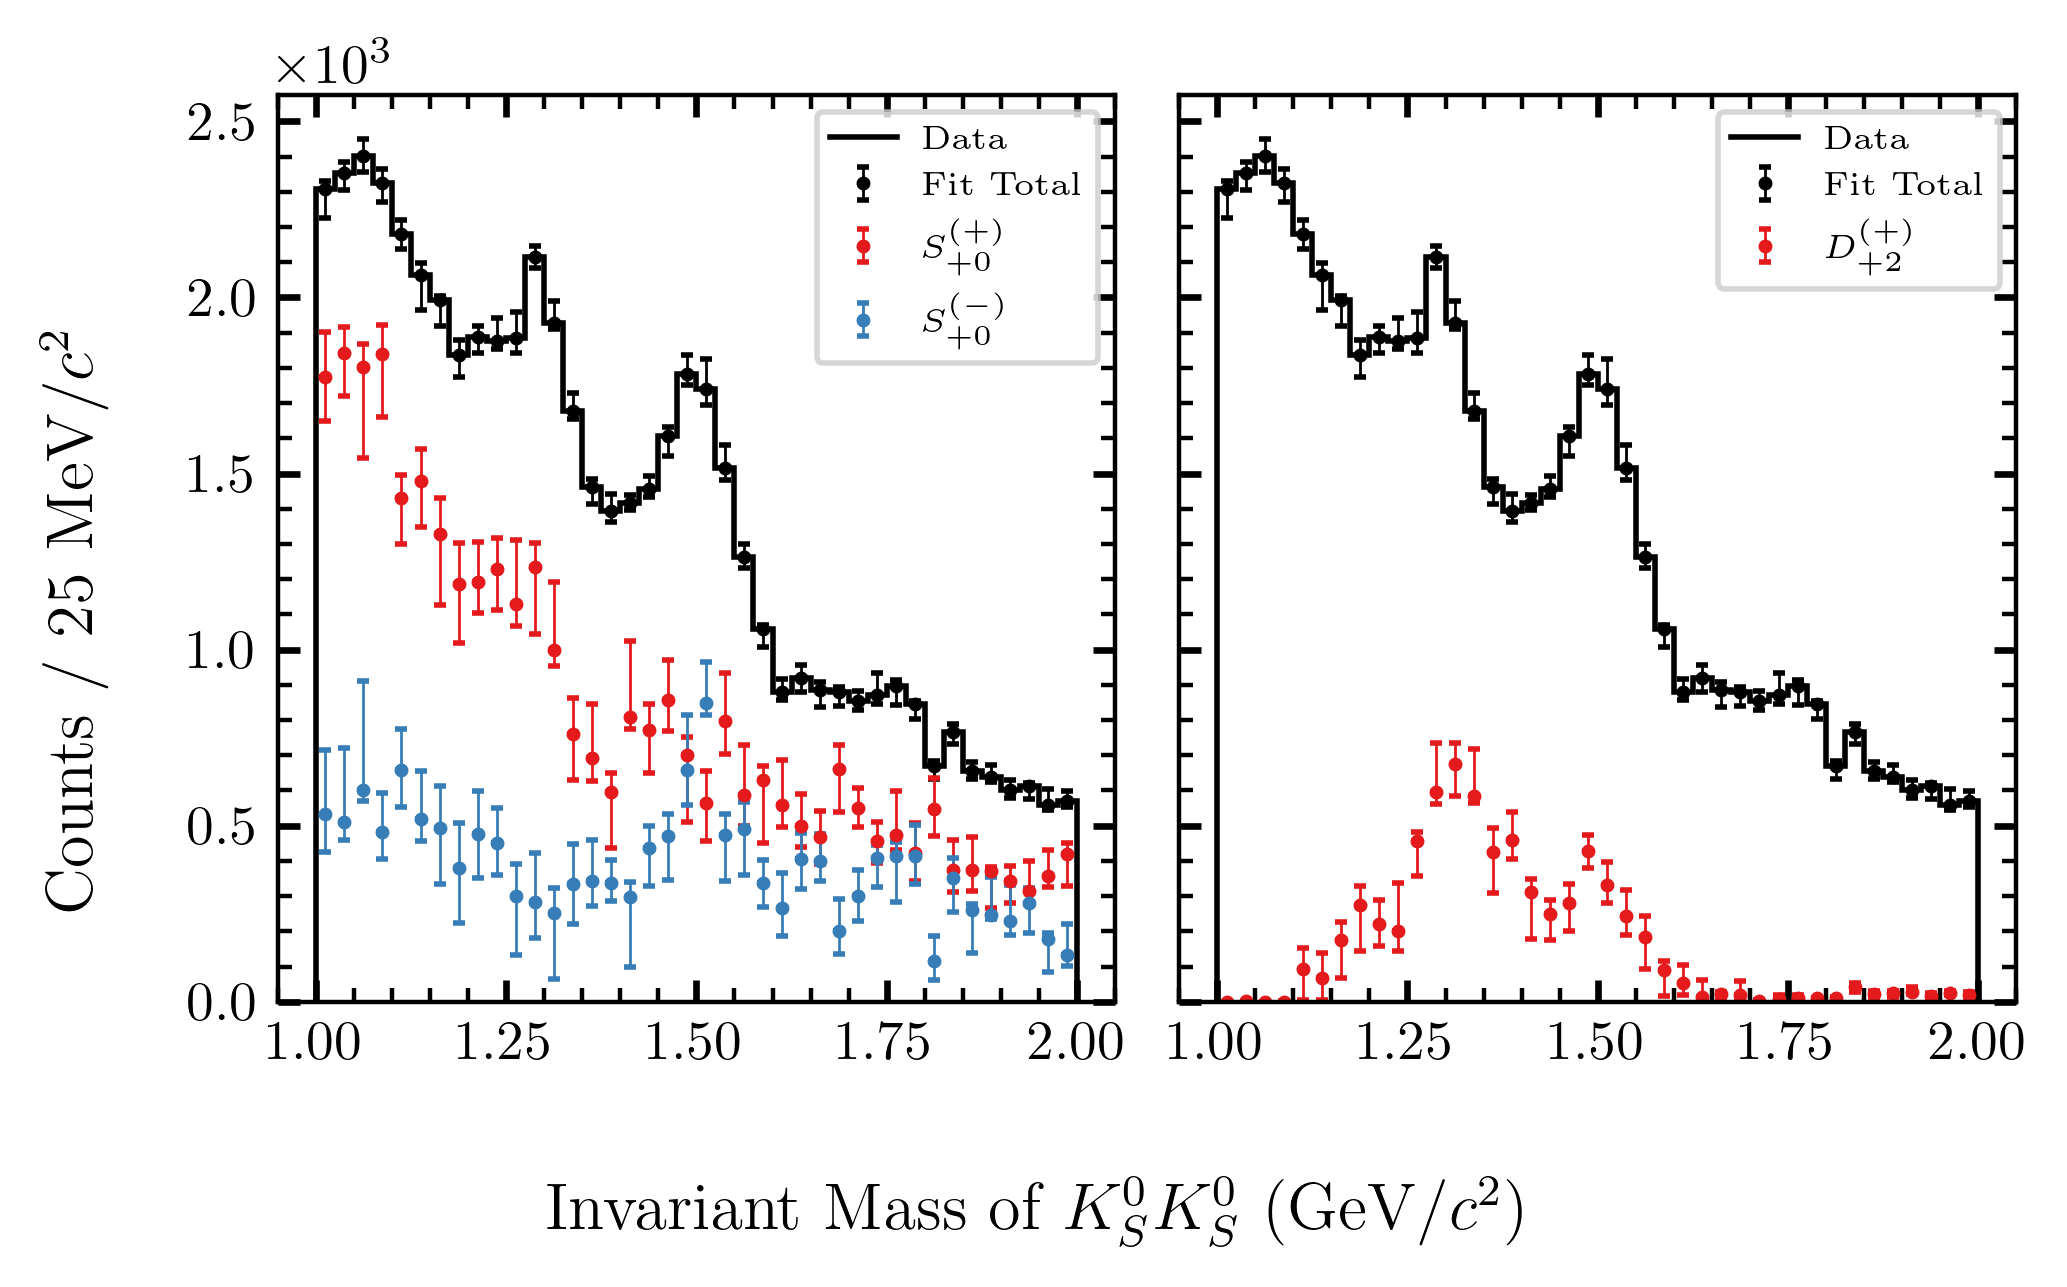
\includegraphics[width=\linewidth]{figures/binned_fit_chisqdof_2.4_splot_D_1s_2b_phase_factor_waves29099_uncertainty_bootstrap-CI-BC.png}
        \caption{$\chi^2_\nu < 2.4$}
    \end{subfigure}

    \vspace{1em}

    \begin{subfigure}{0.8\textwidth}
        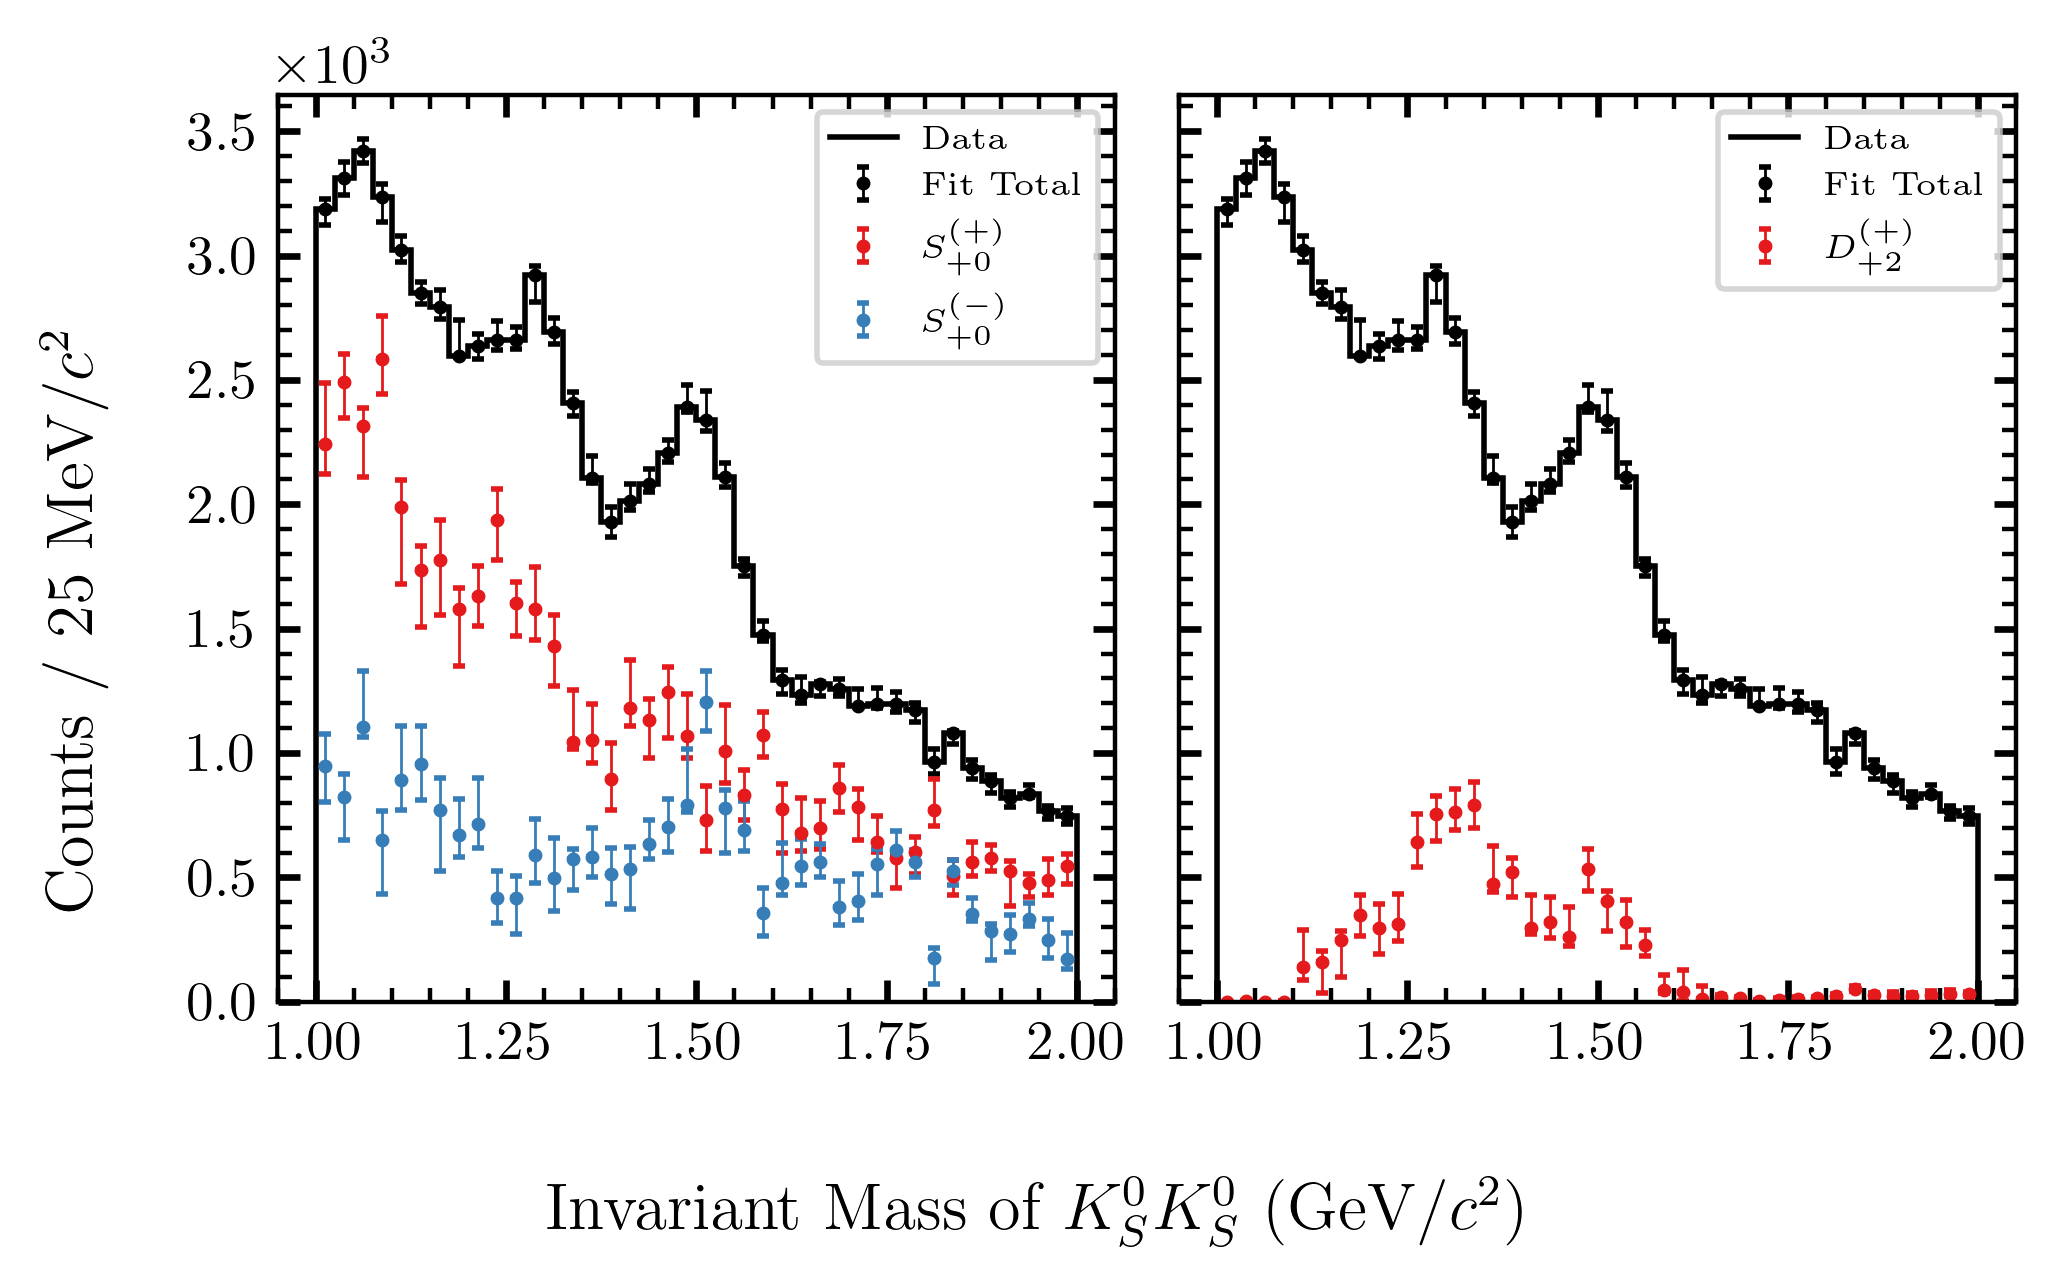
\includegraphics[width=\linewidth]{figures/binned_fit_chisqdof_3.4_splot_D_1s_2b_phase_factor_waves29099_uncertainty_bootstrap-CI-BC.png}
        \caption{$\chi^2_\nu < 3.4$}
    \end{subfigure}

    \vspace{1em}

    \begin{subfigure}{0.45\textwidth}
        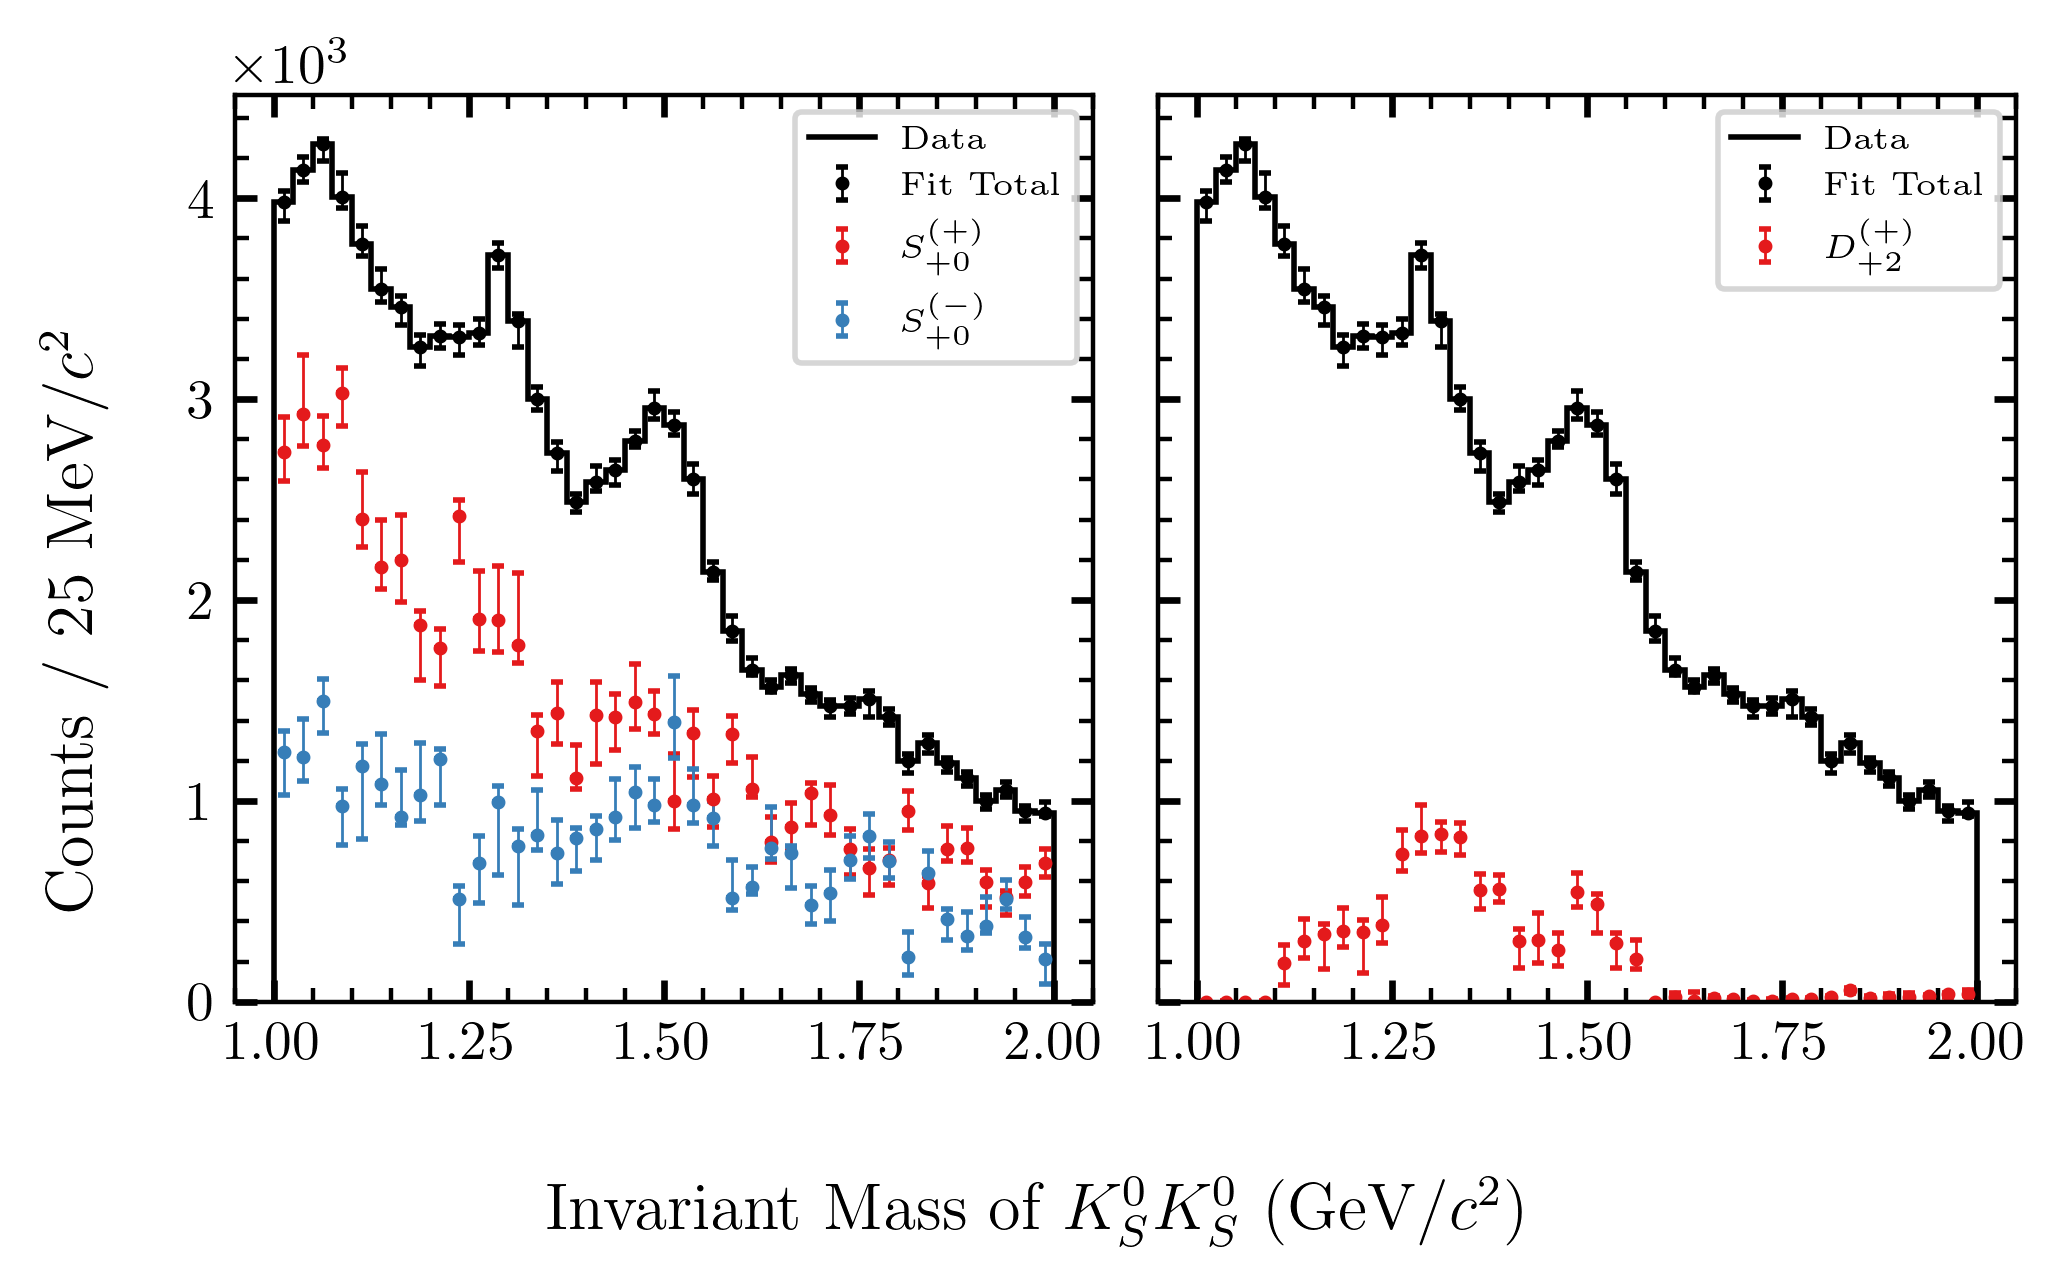
\includegraphics[width=\linewidth]{figures/binned_fit_chisqdof_4.4_splot_D_1s_2b_phase_factor_waves29099_uncertainty_bootstrap-CI-BC.png}
        \caption{$\chi^2_\nu < 4.4$}
    \end{subfigure}
    \hfill
    \begin{subfigure}{0.45\textwidth}
        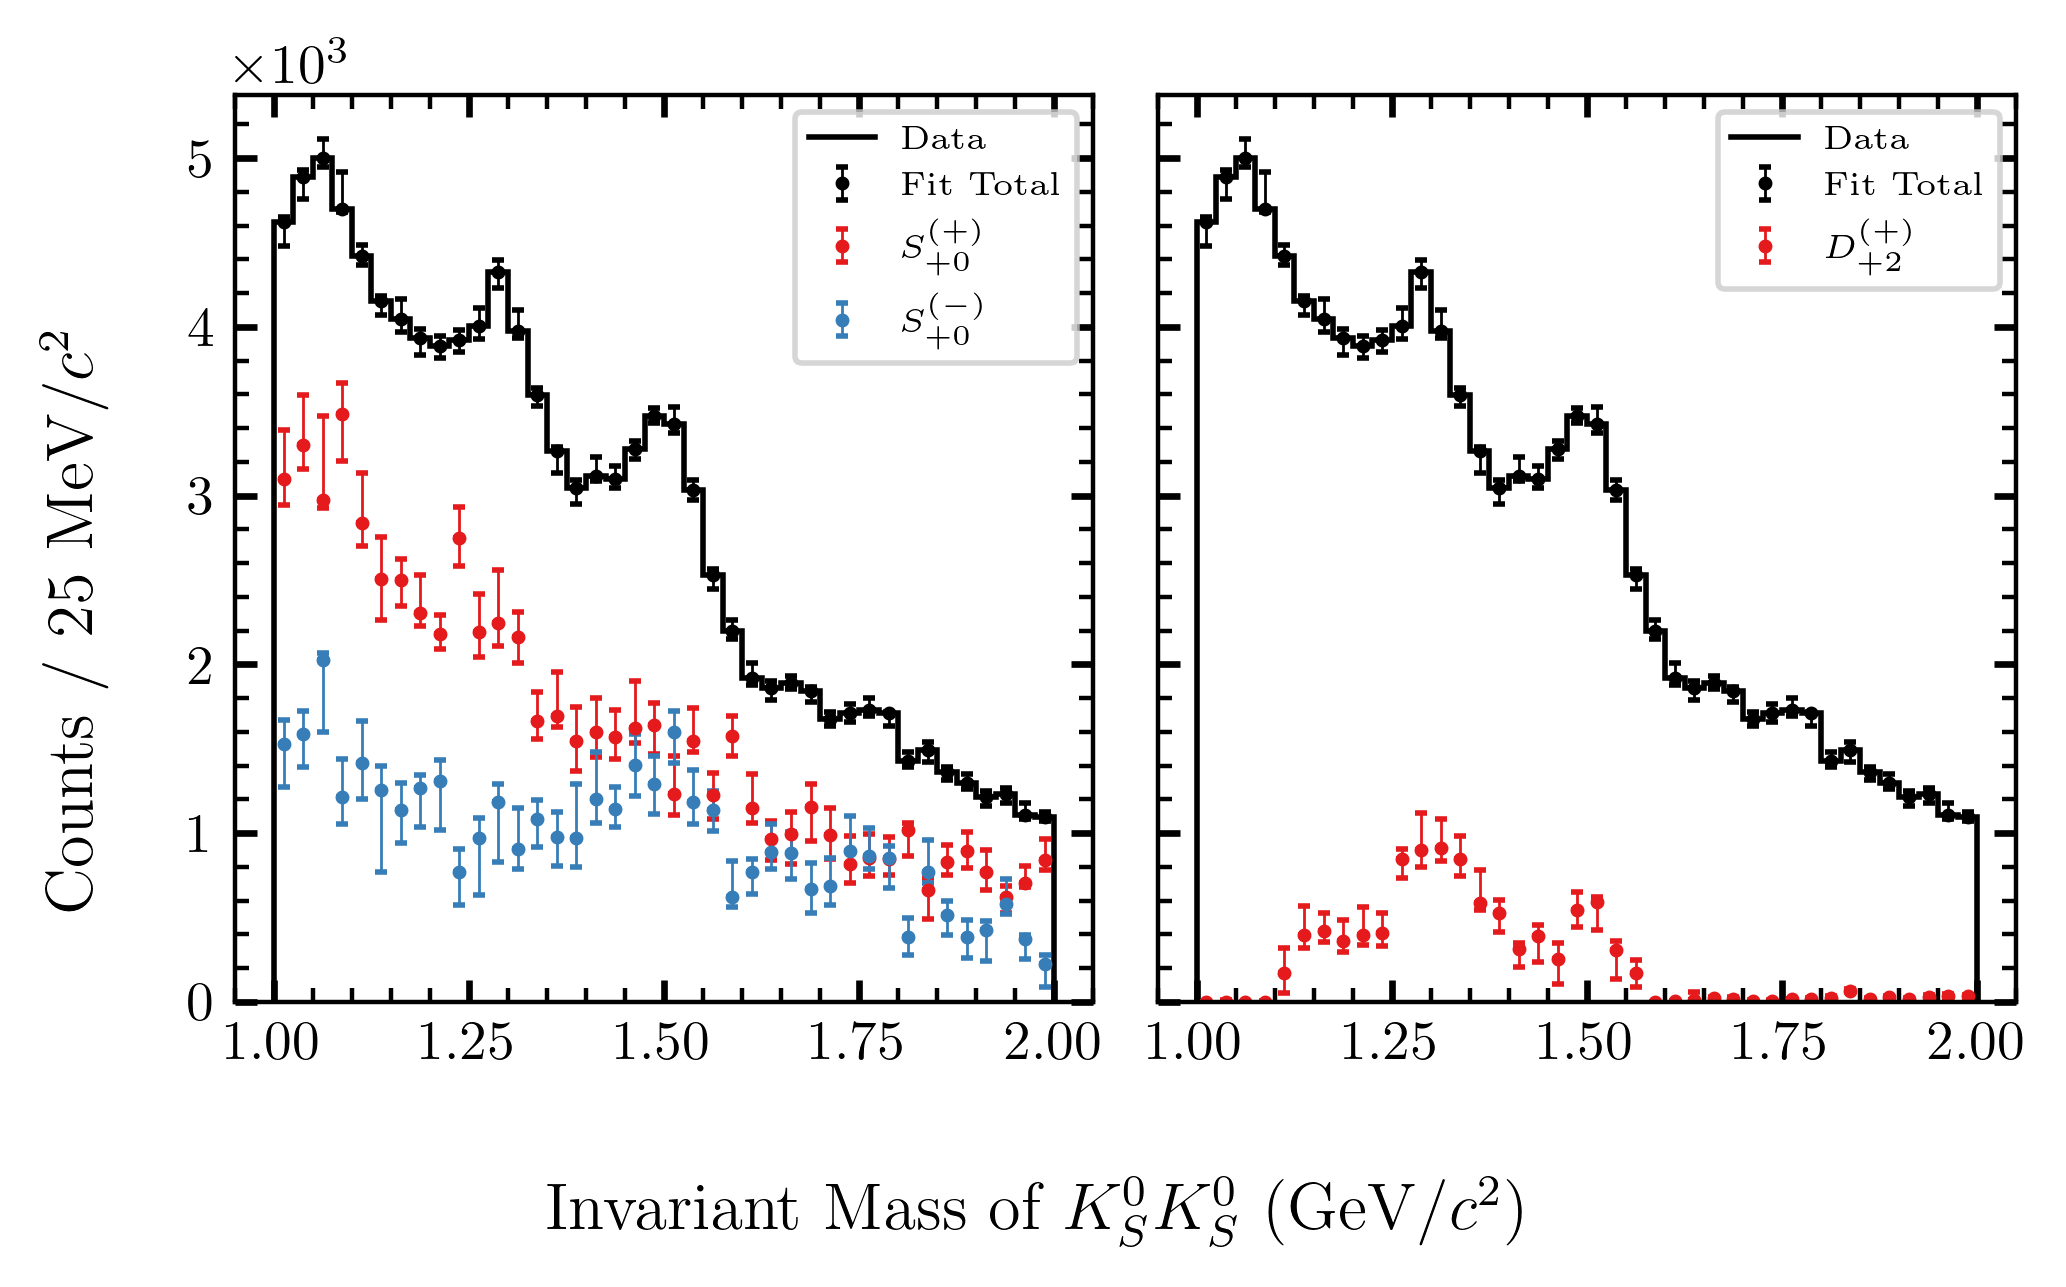
\includegraphics[width=\linewidth]{figures/binned_fit_chisqdof_5.4_splot_D_1s_2b_phase_factor_waves29099_uncertainty_bootstrap-CI-BC.png}
        \caption{$\chi^2_\nu < 5.4$}
    \end{subfigure}

    \caption{Binned fit of $S_{0}^{(+)}$, $S_{0}^{(-)}$, and $D_{+2}^{(+)}$ waves. Bars on each fit point correspond to $68\%$ bias-corrected confidence intervals over $ 30 $ bootstrap iterations.}
    \label{fig:binned-fit-all-Spn-D2p}
\end{figure}

\begin{figure}[htbp]
    \centering
    \begin{subfigure}{0.45\textwidth}
        \includegraphics[width=\linewidth]{figures/binned_and_unbinned_fit_chisqdof_1.4_splot_D_1s_2b_phase_factor_waves491_uncertainty_bootstrap-SE.png}
        \caption{$\chi^2_\nu < 1.4$}
    \end{subfigure}
    \hfill
    \begin{subfigure}{0.45\textwidth}
        \includegraphics[width=\linewidth]{figures/binned_and_unbinned_fit_chisqdof_2.4_splot_D_1s_2b_phase_factor_waves491_uncertainty_bootstrap-SE.png}
        \caption{$\chi^2_\nu < 2.4$}
    \end{subfigure}

    \vspace{1em}

    \begin{subfigure}{0.8\textwidth}
        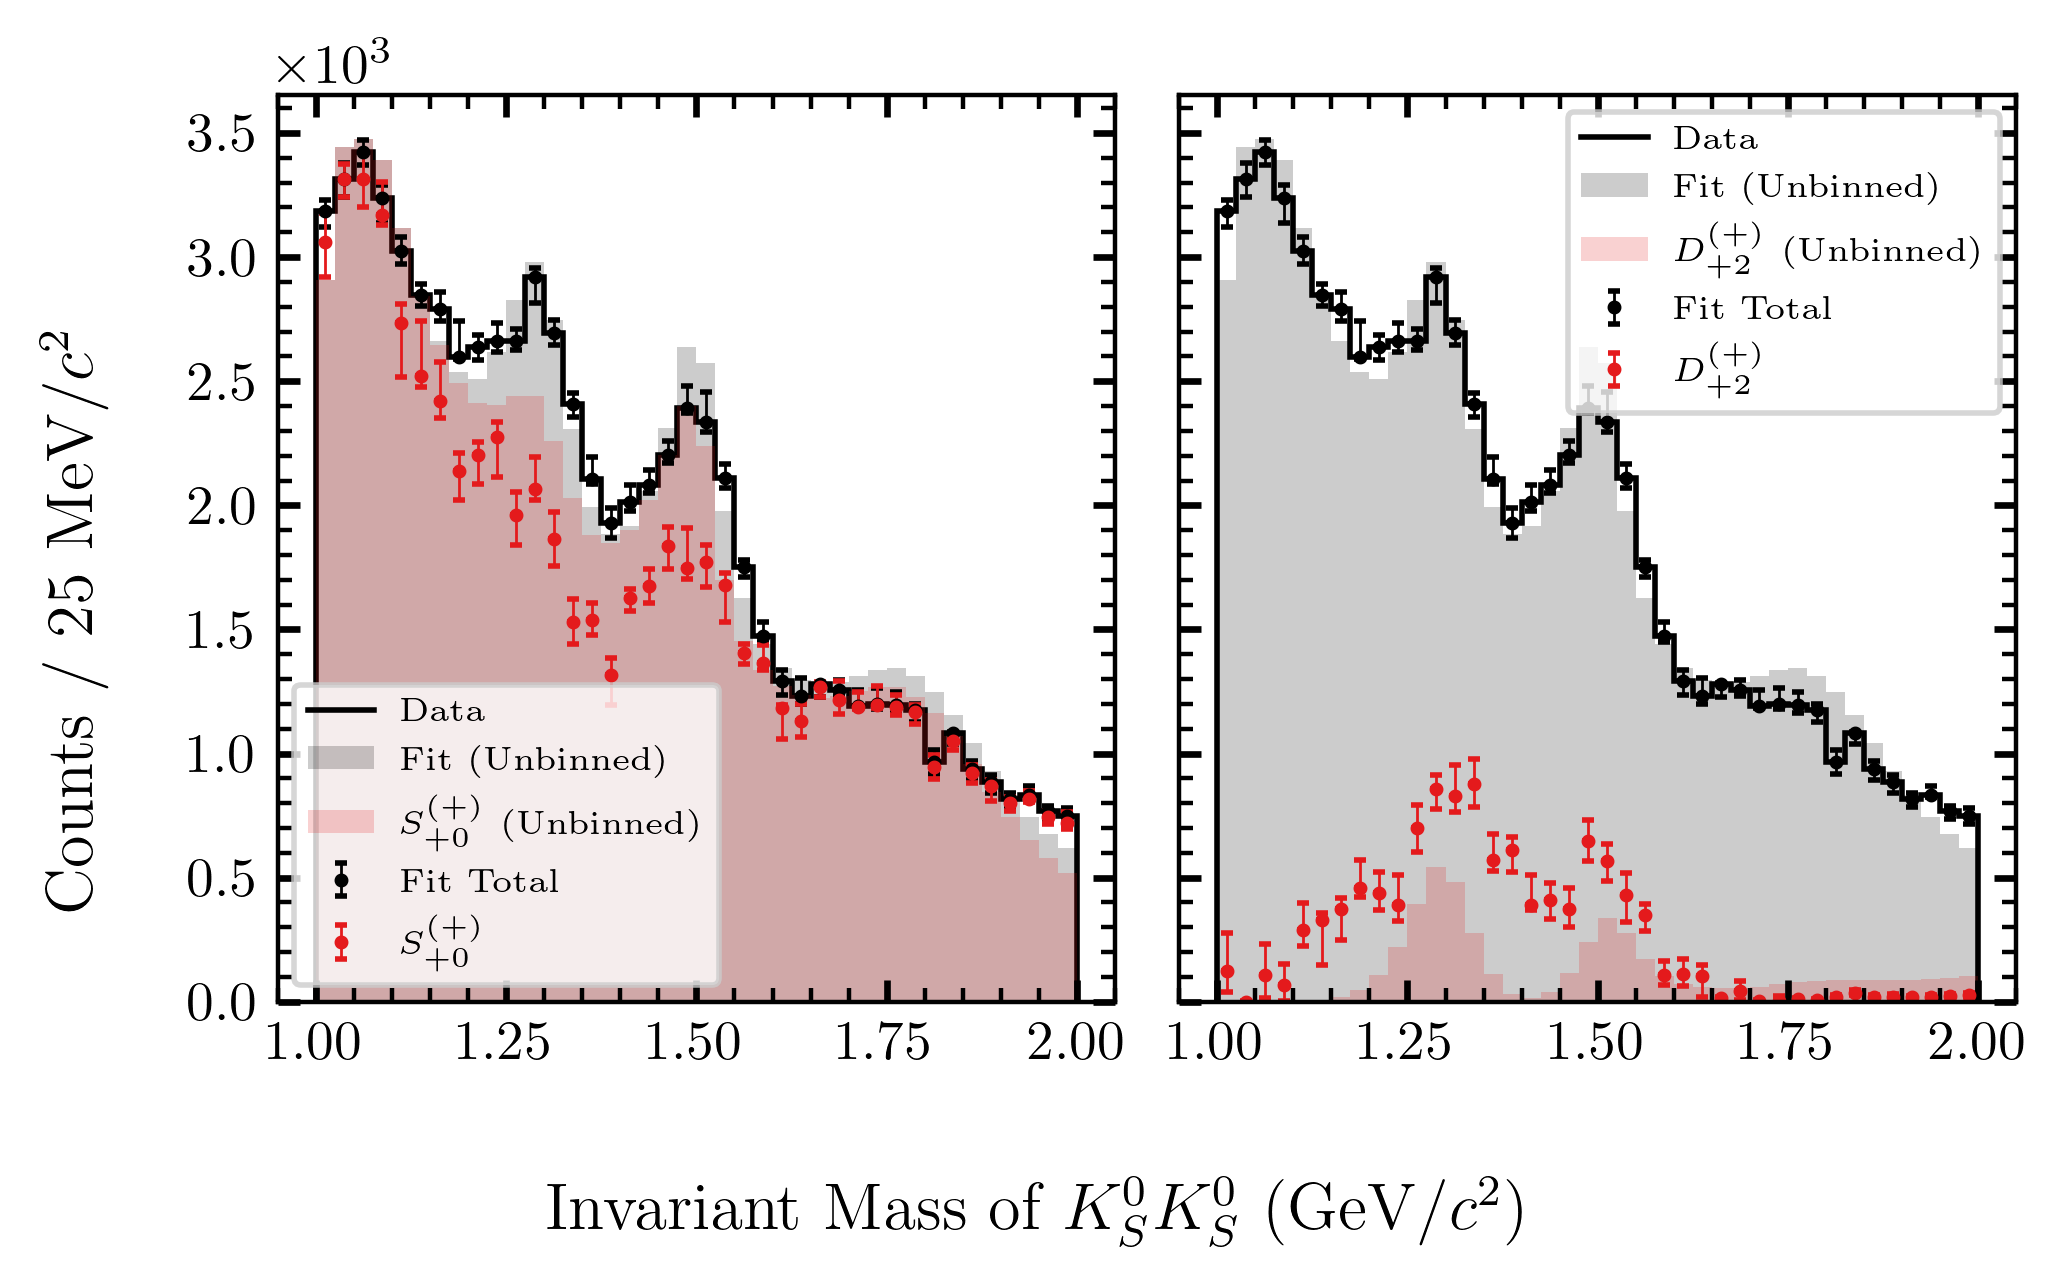
\includegraphics[width=\linewidth]{figures/binned_and_unbinned_fit_chisqdof_3.4_splot_D_1s_2b_phase_factor_waves491_uncertainty_bootstrap-SE.png}
        \caption{$\chi^2_\nu < 3.4$}
    \end{subfigure}

    \vspace{1em}

    \begin{subfigure}{0.45\textwidth}
        \includegraphics[width=\linewidth]{figures/binned_and_unbinned_fit_chisqdof_4.4_splot_D_1s_2b_phase_factor_waves491_uncertainty_bootstrap-SE.png}
        \caption{$\chi^2_\nu < 4.4$}
    \end{subfigure}
    \hfill
    \begin{subfigure}{0.45\textwidth}
        \includegraphics[width=\linewidth]{figures/binned_and_unbinned_fit_chisqdof_5.4_splot_D_1s_2b_phase_factor_waves491_uncertainty_bootstrap-SE.png}
        \caption{$\chi^2_\nu < 5.4$}
    \end{subfigure}

    \caption{Mass-independent (binned) and mass-dependent (unbinned) fit of $S_{0}^{(+)}$ and $D_{+2}^{(+)}$ waves. Bars on each fit point correspond to $68\%$ bias-corrected confidence intervals over $ 30 $ bootstrap iterations.}
    \label{fig:unbinned-fit-all-Sp-D2p}
\end{figure}

\begin{figure}[htbp]
    \centering
    \begin{subfigure}{0.45\textwidth}
        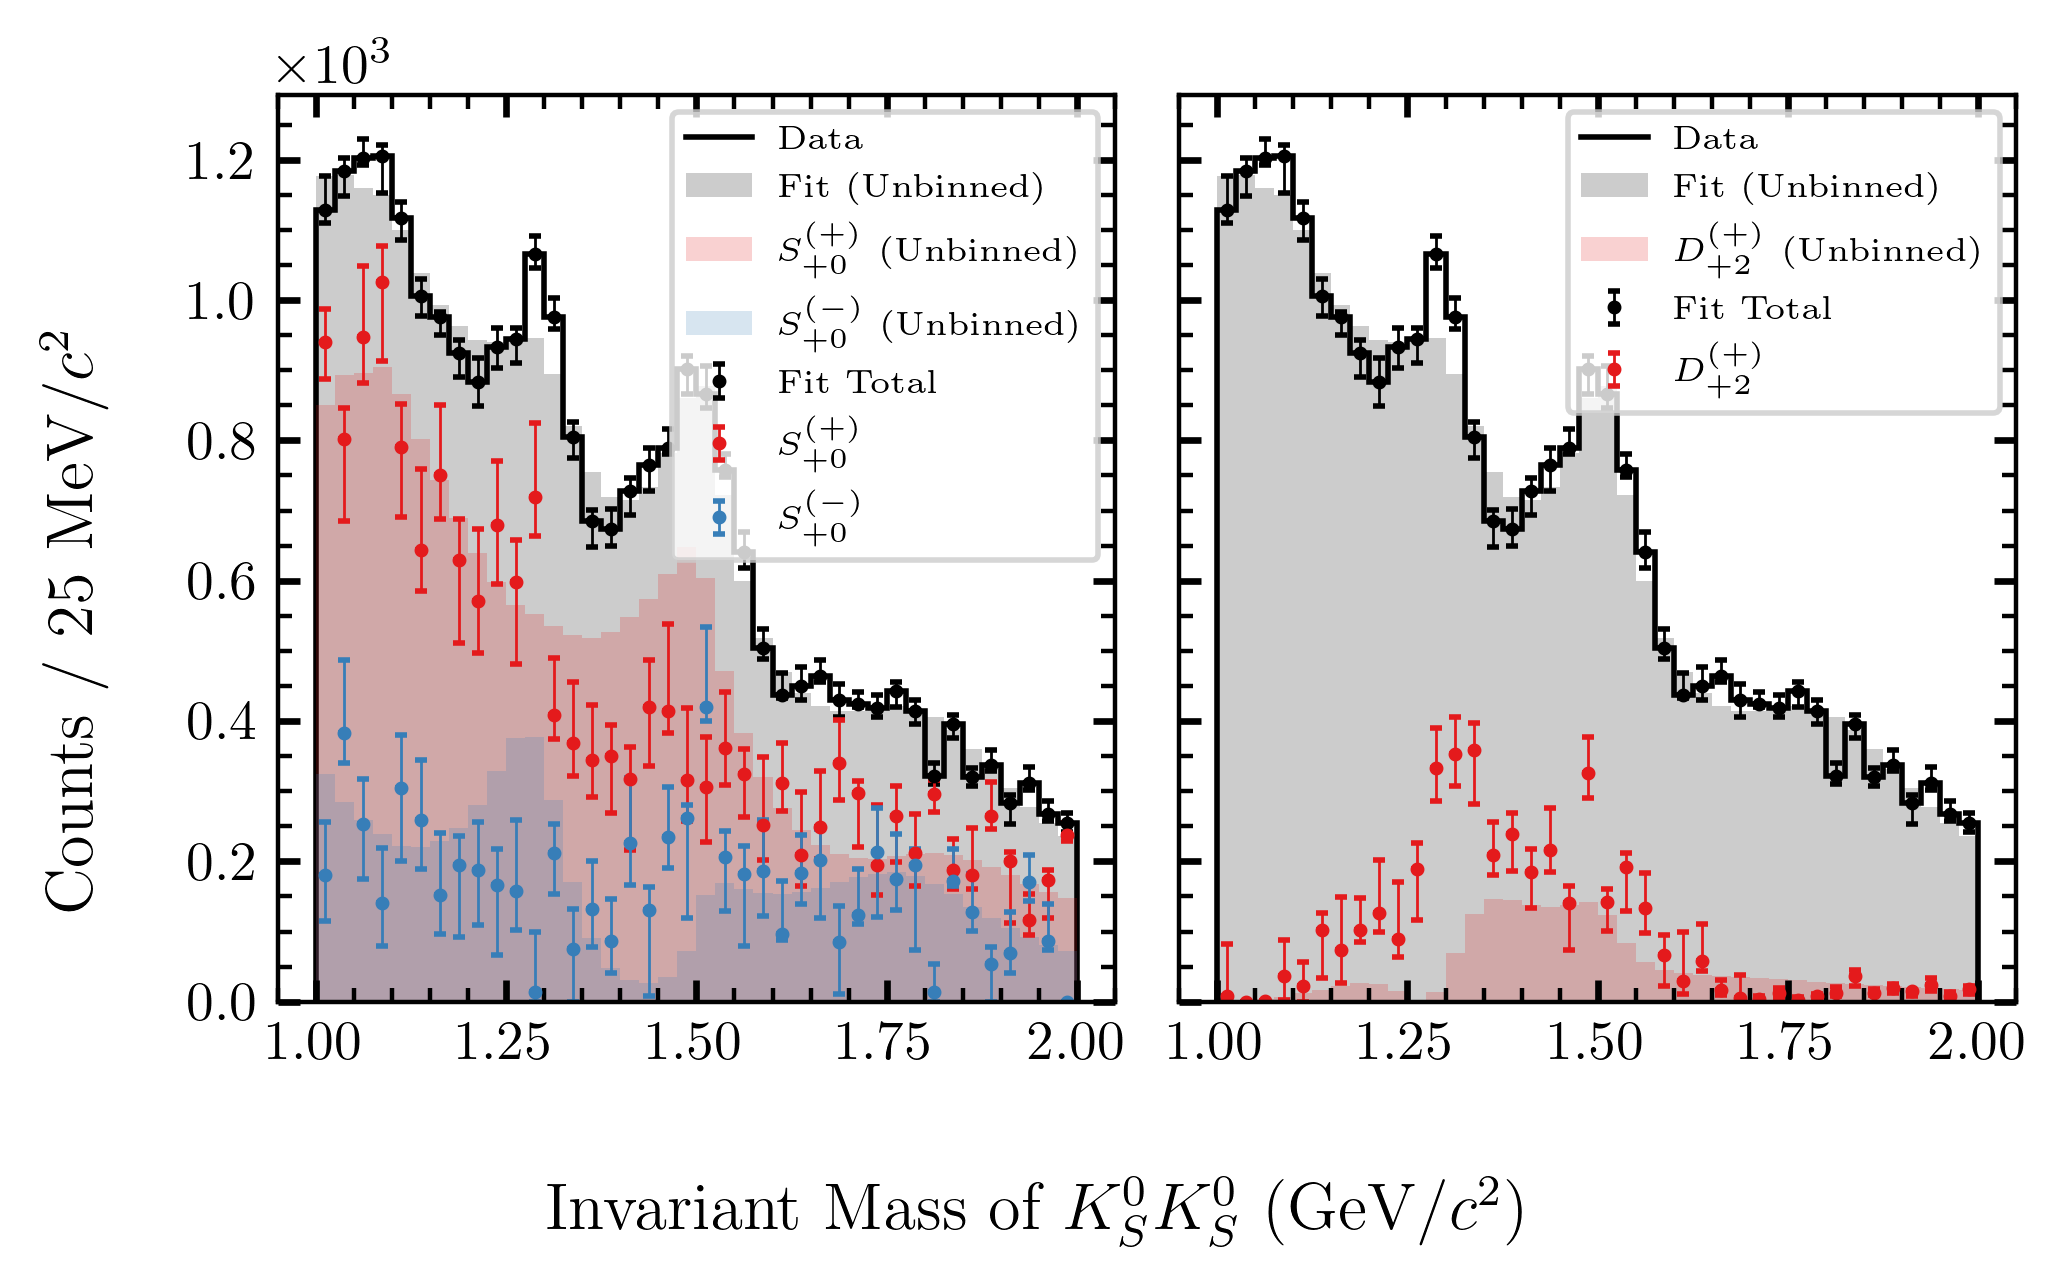
\includegraphics[width=\linewidth]{figures/binned_and_unbinned_fit_chisqdof_1.4_splot_D_1s_2b_phase_factor_waves29099_uncertainty_bootstrap-SE.png}
        \caption{$\chi^2_\nu < 1.4$}
    \end{subfigure}
    \hfill
    \begin{subfigure}{0.45\textwidth}
        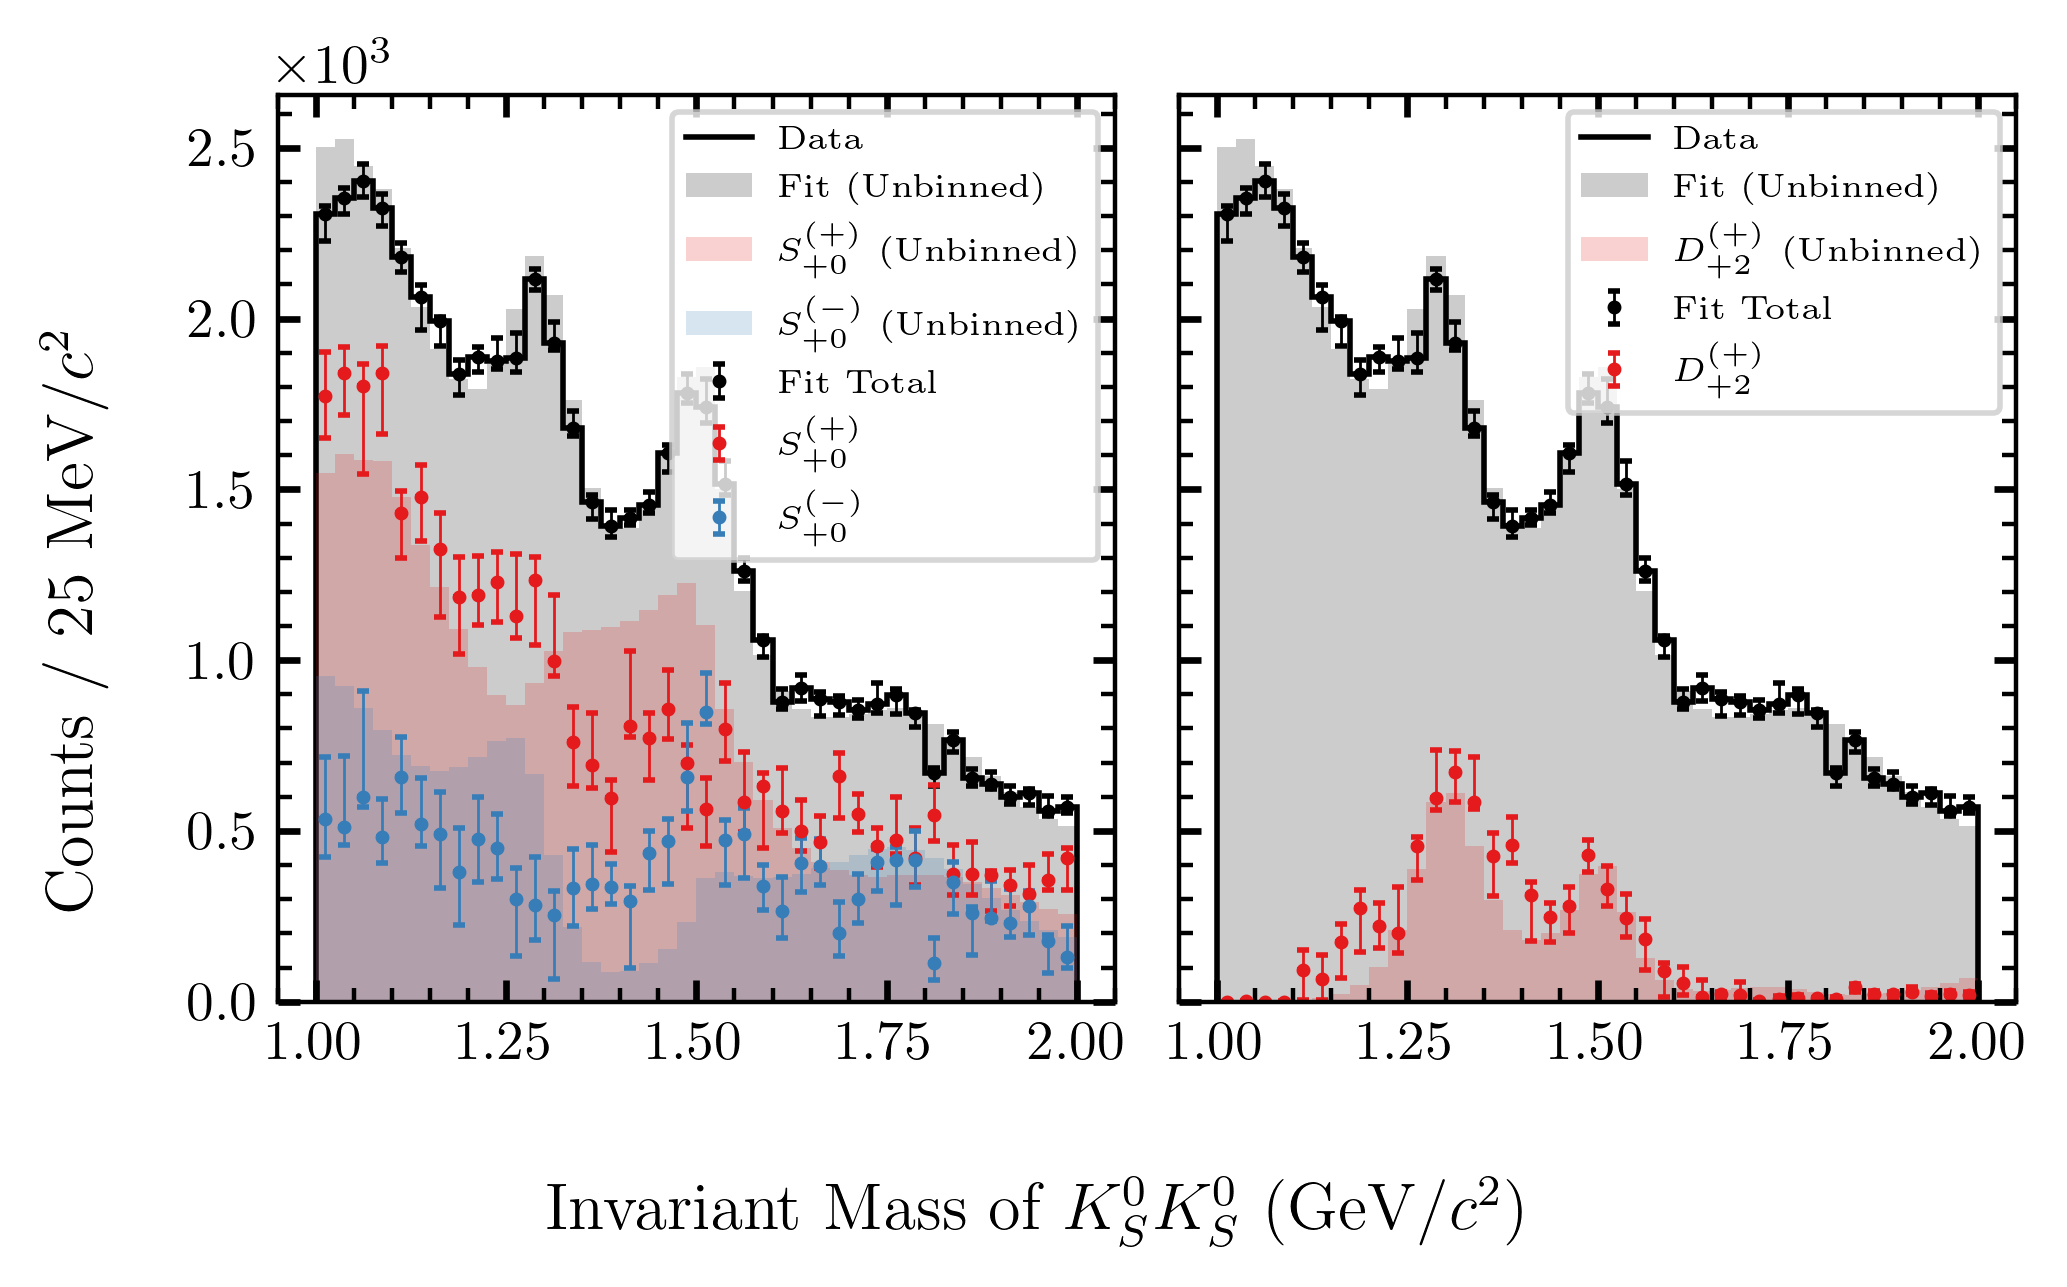
\includegraphics[width=\linewidth]{figures/binned_and_unbinned_fit_chisqdof_2.4_splot_D_1s_2b_phase_factor_waves29099_uncertainty_bootstrap-SE.png}
        \caption{$\chi^2_\nu < 2.4$}
    \end{subfigure}

    \vspace{1em}

    \begin{subfigure}{0.8\textwidth}
        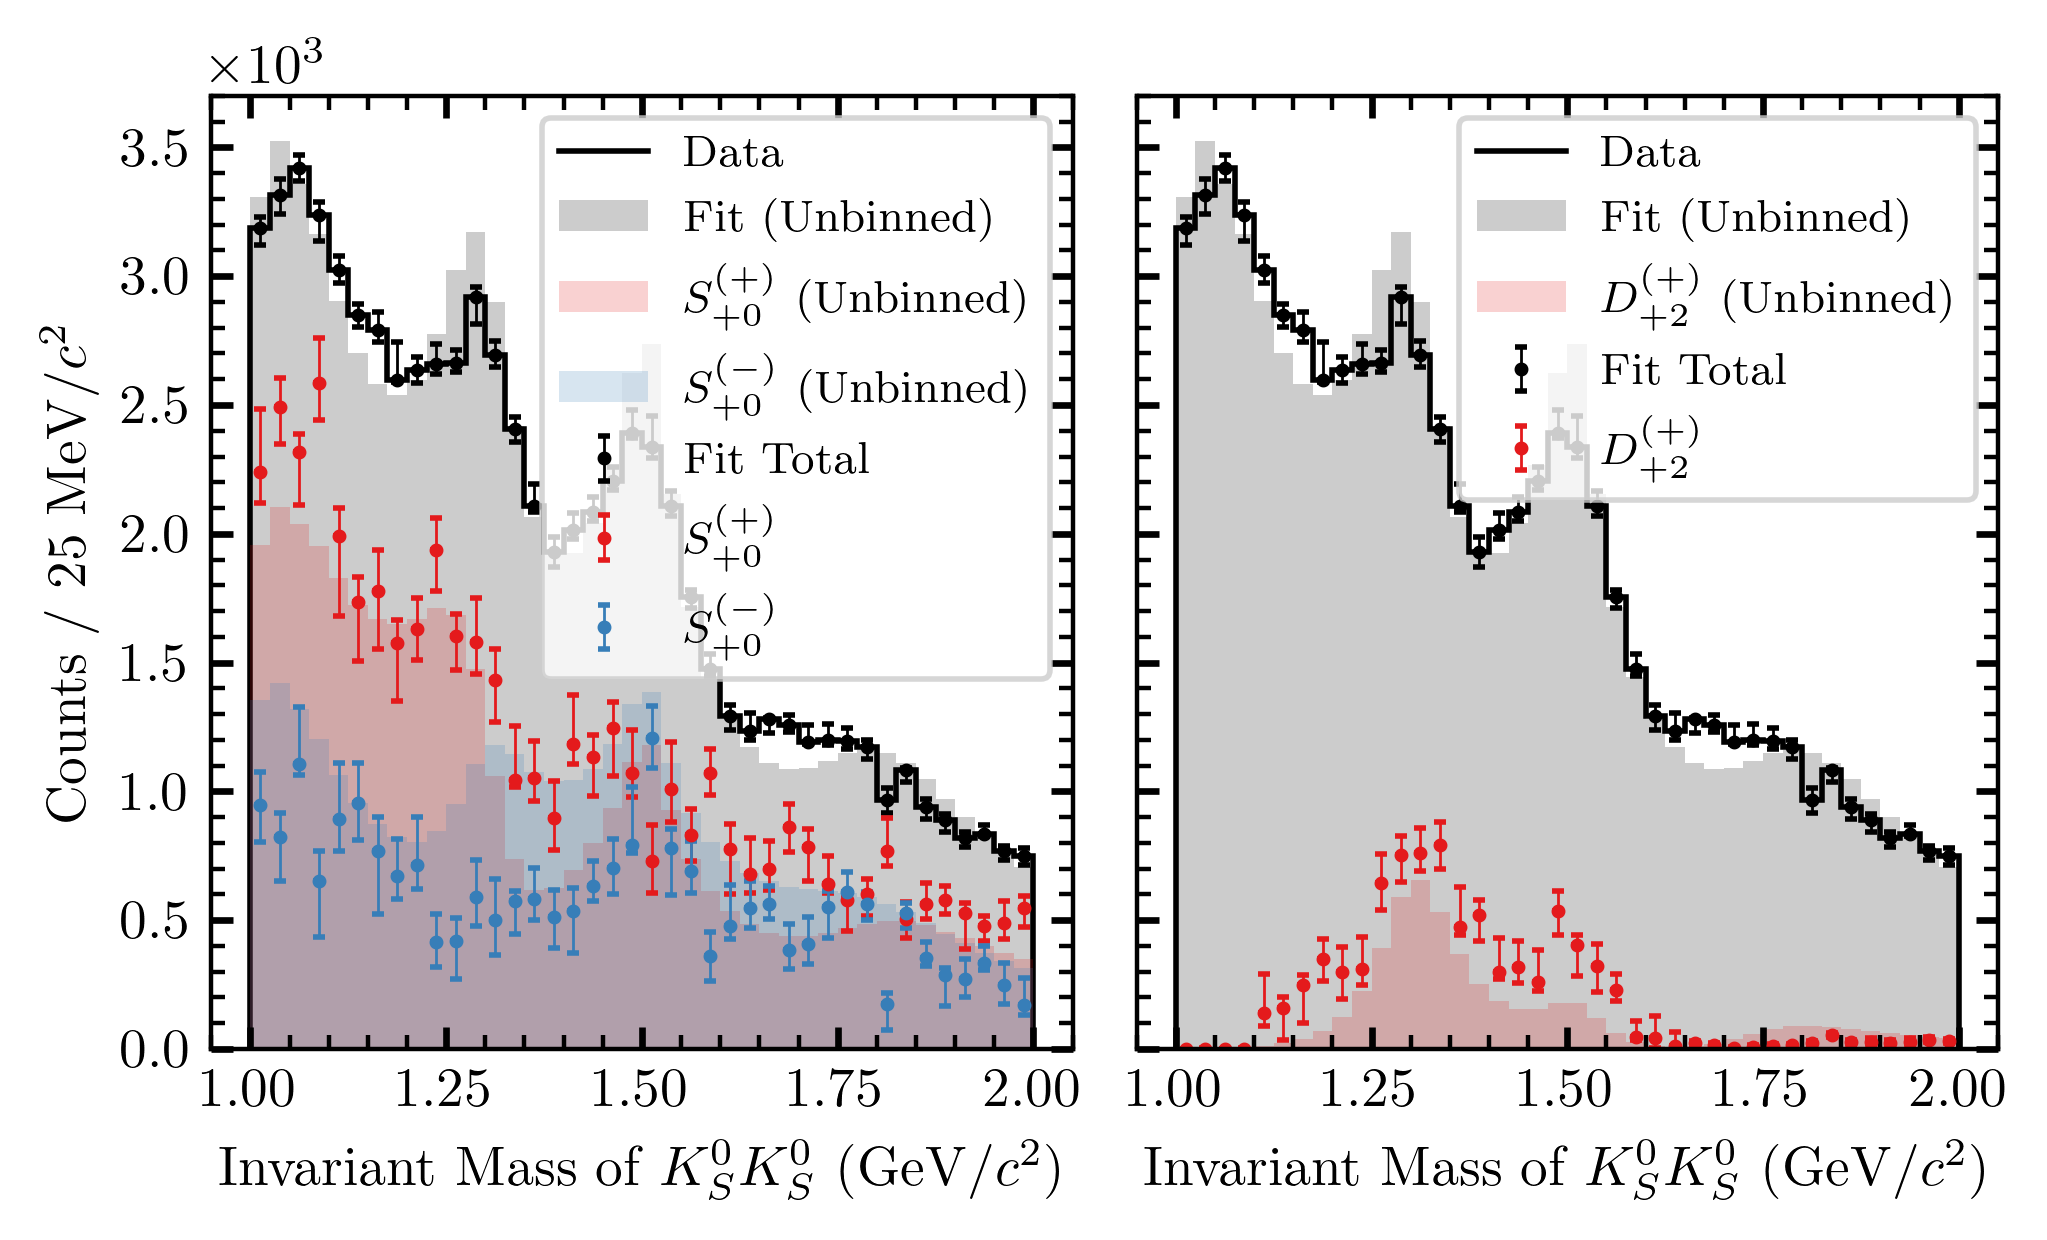
\includegraphics[width=\linewidth]{figures/binned_and_unbinned_fit_chisqdof_3.4_splot_D_1s_2b_phase_factor_waves29099_uncertainty_bootstrap-SE.png}
        \caption{$\chi^2_\nu < 3.4$}
    \end{subfigure}

    \vspace{1em}

    \begin{subfigure}{0.45\textwidth}
        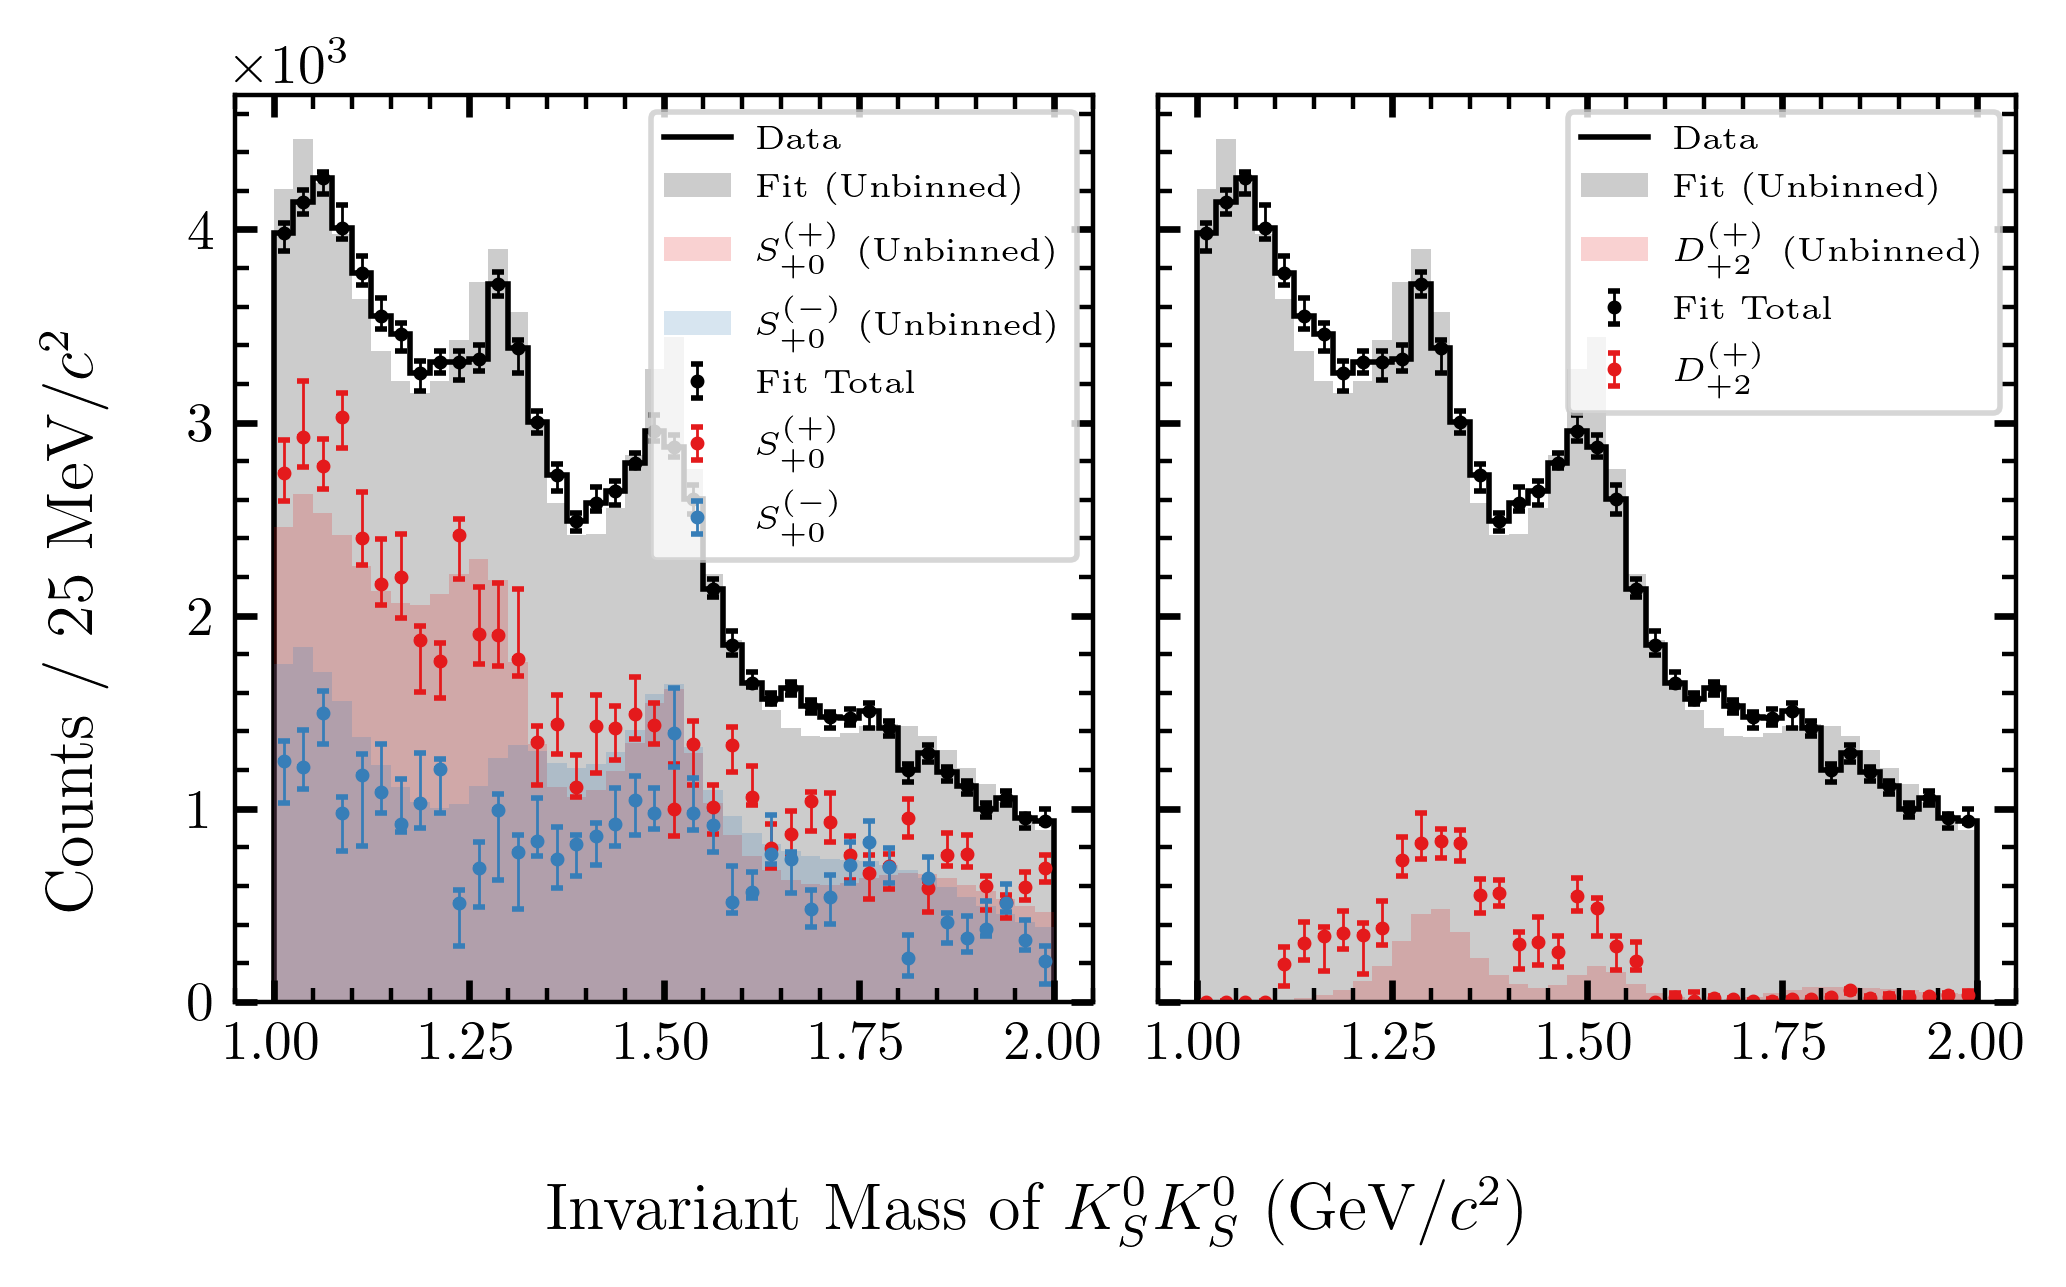
\includegraphics[width=\linewidth]{figures/binned_and_unbinned_fit_chisqdof_4.4_splot_D_1s_2b_phase_factor_waves29099_uncertainty_bootstrap-SE.png}
        \caption{$\chi^2_\nu < 4.4$}
    \end{subfigure}
    \hfill
    \begin{subfigure}{0.45\textwidth}
        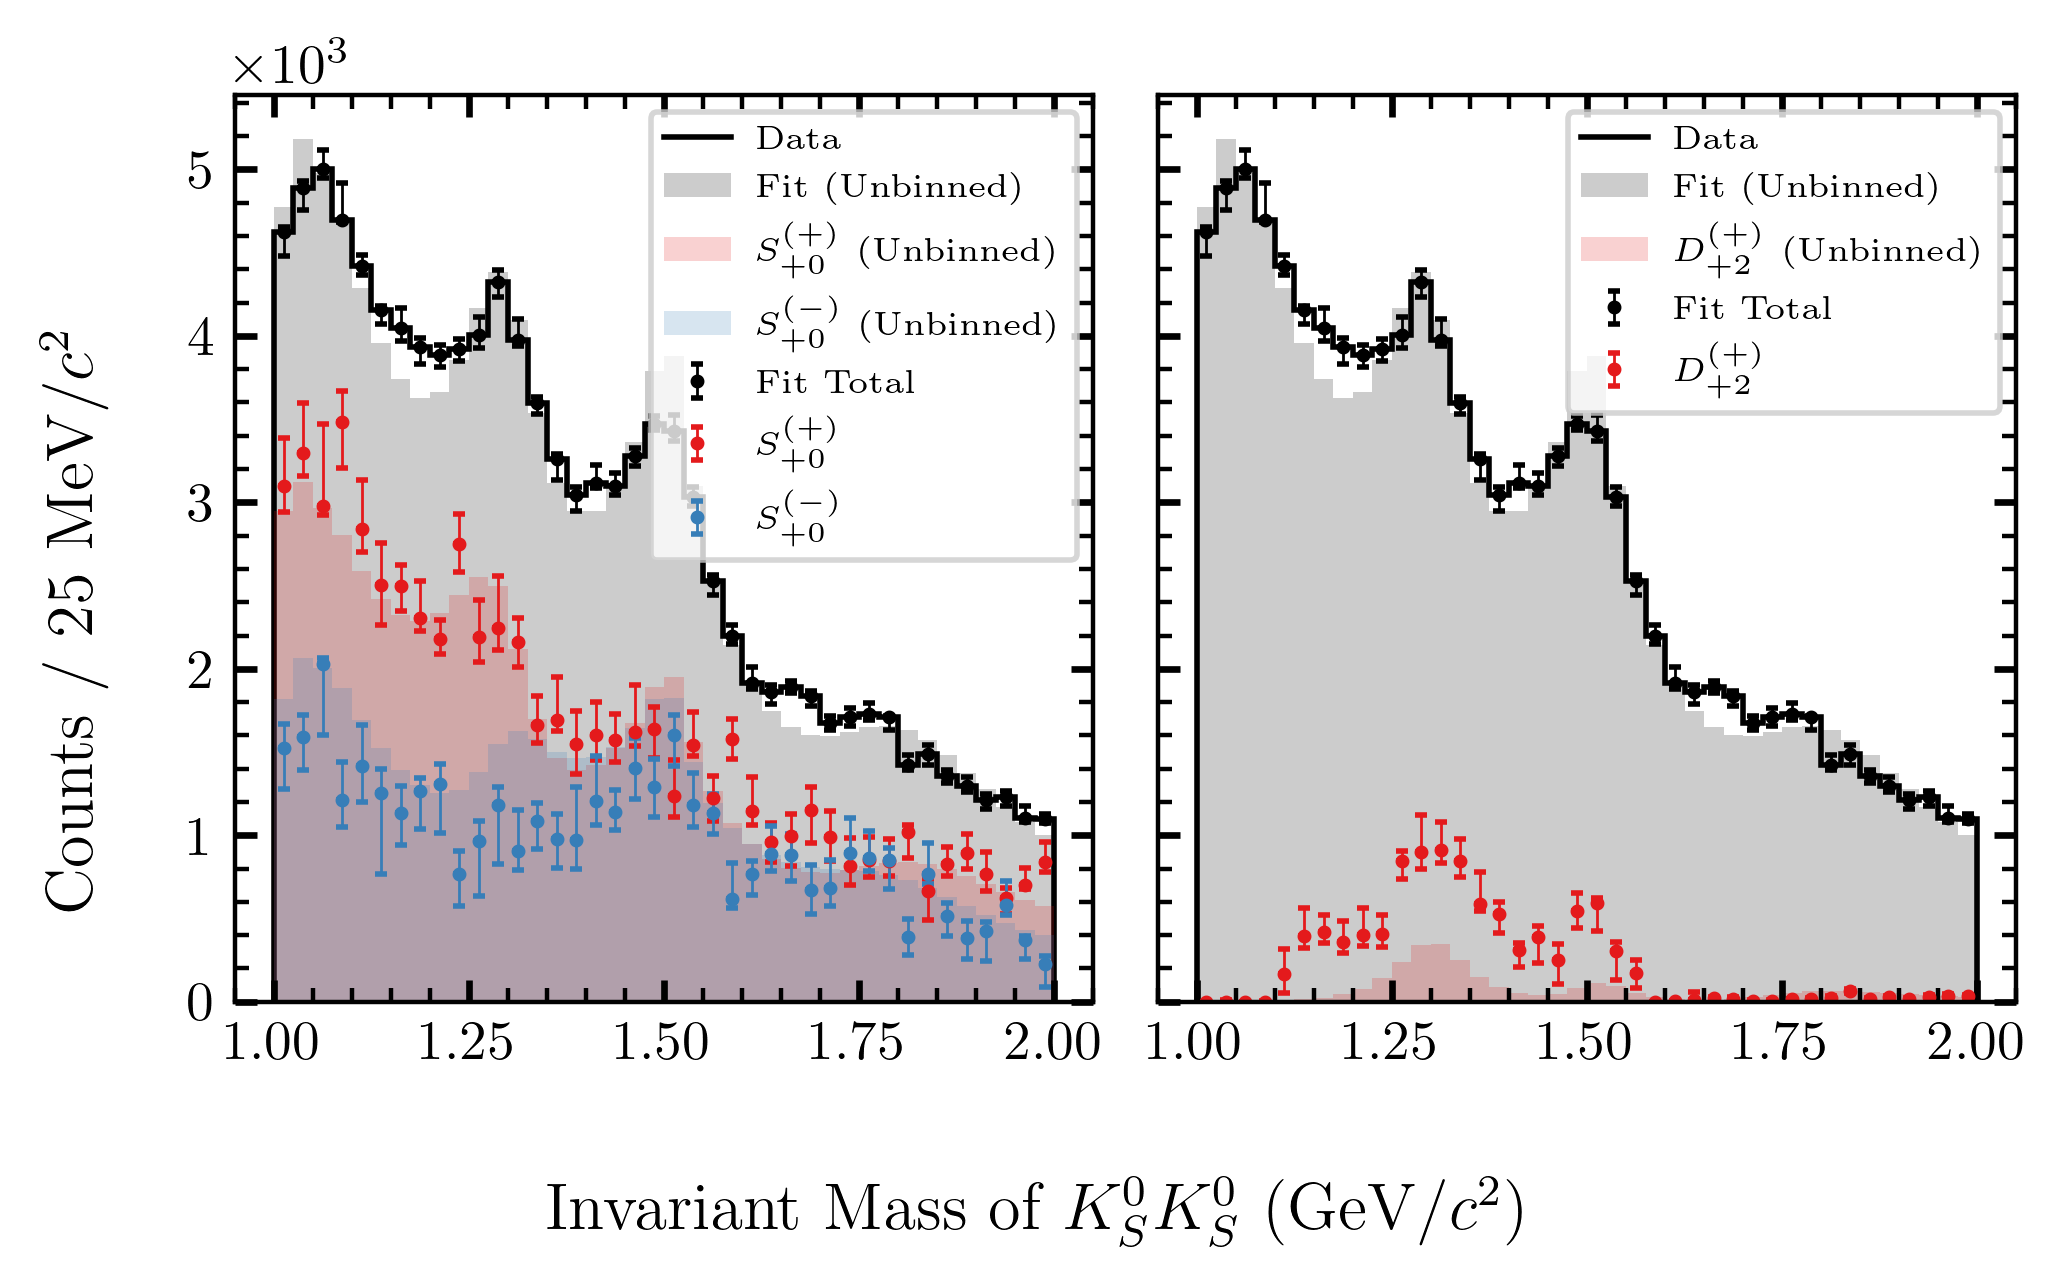
\includegraphics[width=\linewidth]{figures/binned_and_unbinned_fit_chisqdof_5.4_splot_D_1s_2b_phase_factor_waves29099_uncertainty_bootstrap-SE.png}
        \caption{$\chi^2_\nu < 5.4$}
    \end{subfigure}

    \caption{Mass-independent (binned) and mass-dependent (unbinned) fit of $S_{0}^{(+)}$, $S_{0}^{(-)}$, and $D_{+2}^{(+)}$ waves. Bars on each fit point correspond to $68\%$ bias-corrected confidence intervals over $ 30 $ bootstrap iterations.}
    \label{fig:unbinned-fit-all-Spn-D2p}
\end{figure}

\begin{figure}[htbp]
    \centering
    \begin{subfigure}{0.45\textwidth}
        \includegraphics[width=\linewidth]{figures/guided_fit_chisqdof_1.4_splot_D_1s_2b_phase_factor_waves491_uncertainty_bootstrap-SE.png}
        \caption{$\chi^2_\nu < 1.4$}
    \end{subfigure}
    \hfill
    \begin{subfigure}{0.45\textwidth}
        \includegraphics[width=\linewidth]{figures/guided_fit_chisqdof_2.4_splot_D_1s_2b_phase_factor_waves491_uncertainty_bootstrap-SE.png}
        \caption{$\chi^2_\nu < 2.4$}
    \end{subfigure}

    \vspace{1em}

    \begin{subfigure}{0.8\textwidth}
        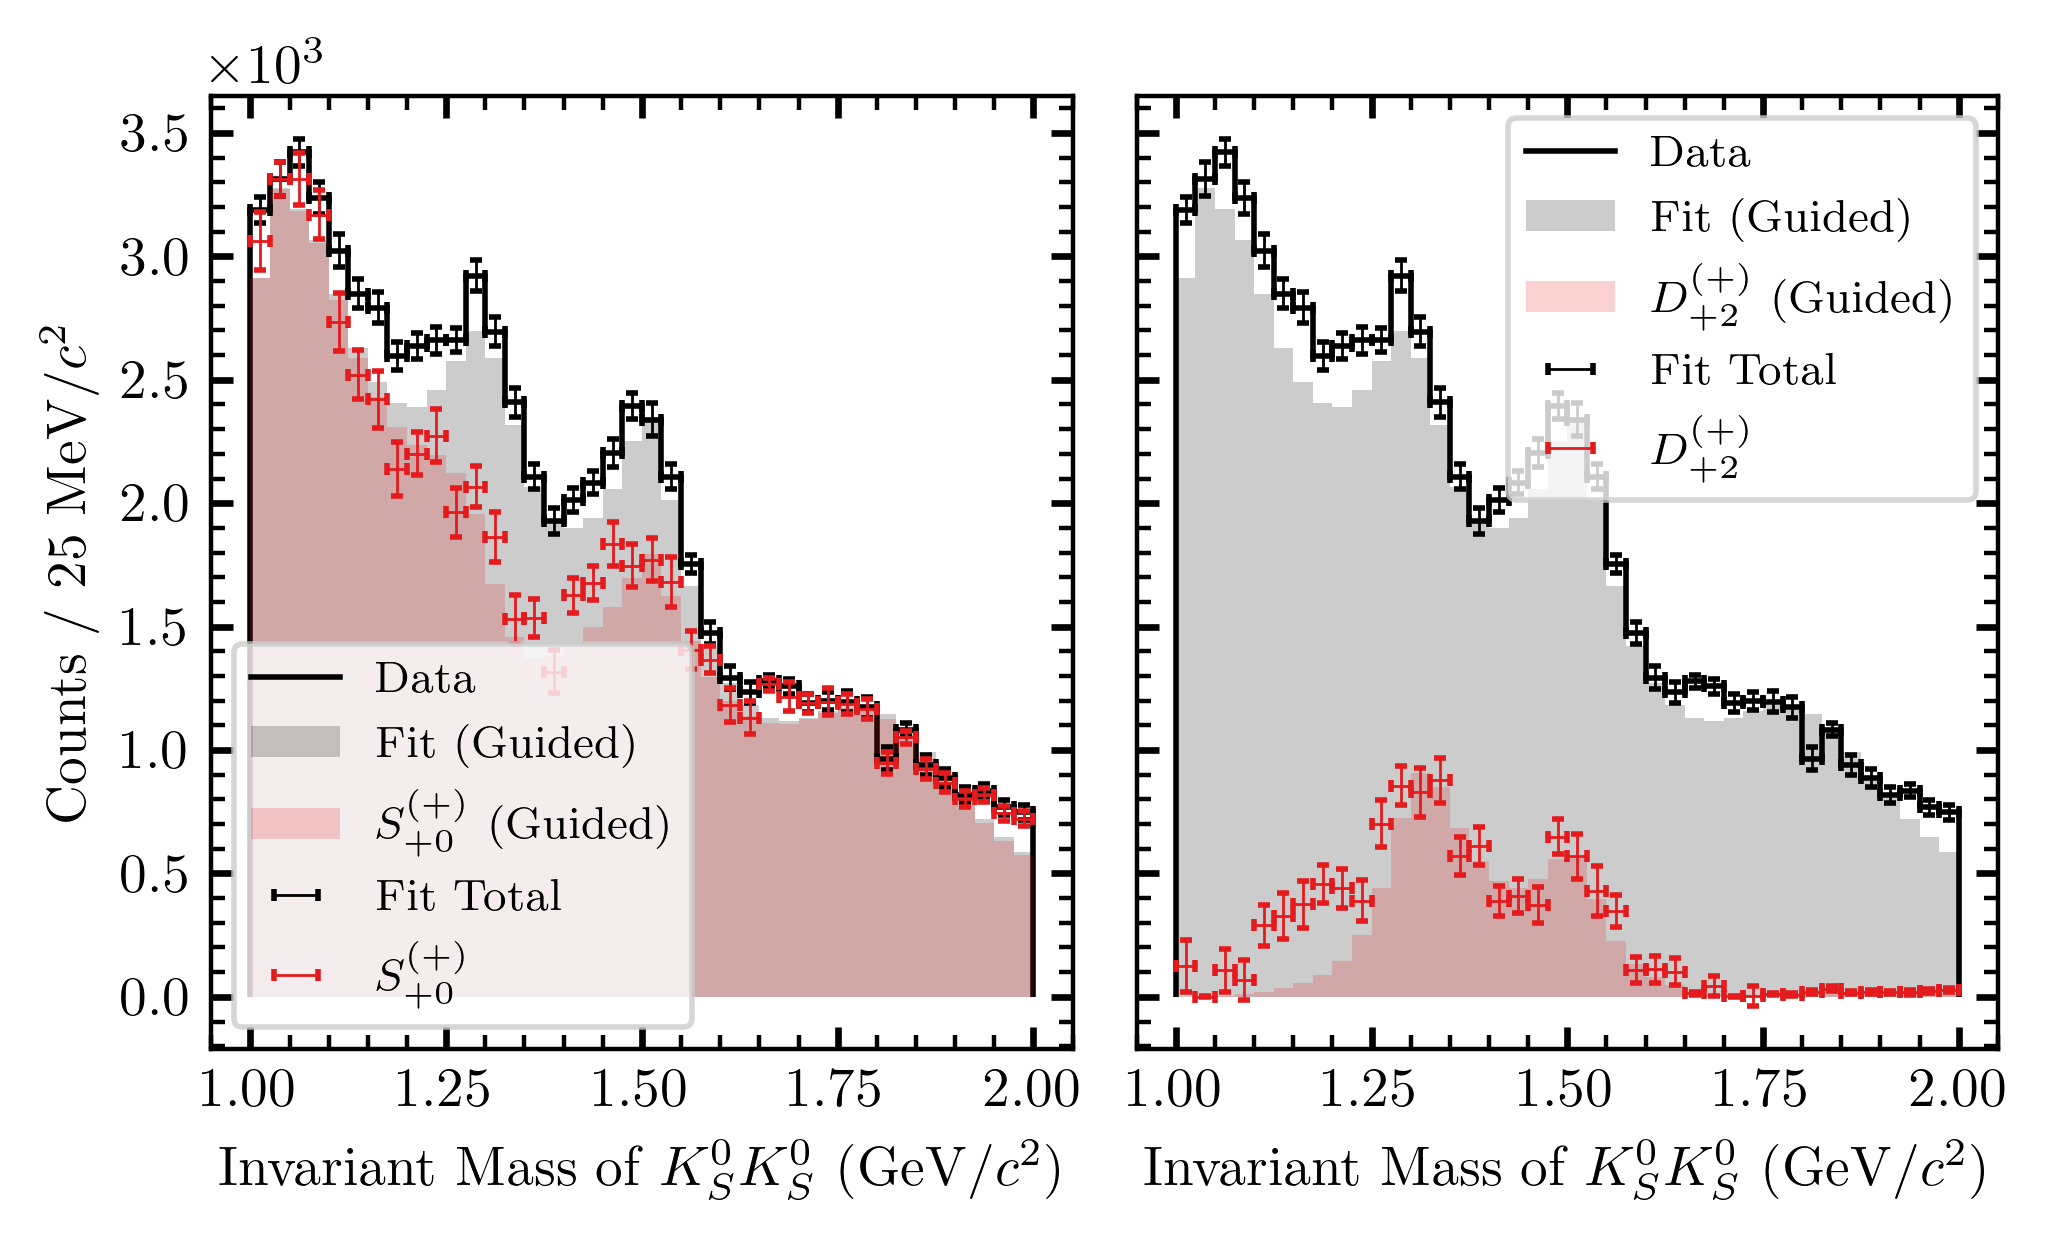
\includegraphics[width=\linewidth]{figures/guided_fit_chisqdof_3.4_splot_D_1s_2b_phase_factor_waves491_uncertainty_bootstrap-SE.png}
        \caption{$\chi^2_\nu < 3.4$}
    \end{subfigure}

    \vspace{1em}

    \begin{subfigure}{0.45\textwidth}
        \includegraphics[width=\linewidth]{figures/guided_fit_chisqdof_4.4_splot_D_1s_2b_phase_factor_waves491_uncertainty_bootstrap-SE.png}
        \caption{$\chi^2_\nu < 4.4$}
    \end{subfigure}
    \hfill
    \begin{subfigure}{0.45\textwidth}
        \includegraphics[width=\linewidth]{figures/guided_fit_chisqdof_5.4_splot_D_1s_2b_phase_factor_waves491_uncertainty_bootstrap-SE.png}
        \caption{$\chi^2_\nu < 5.4$}
    \end{subfigure}

    \caption{The state of the guided fit to $S_{0}^{(+)}$ and $D_{+2}^{(+)}$ waves after the guided step. Bars on each fit point correspond to the standard error on the intensity from $ 30 $ bootstrap iterations.}
    \label{fig:guided-fit-all-Sp-D2p}
\end{figure}

\begin{figure}[htbp]
    \centering
    \begin{subfigure}{0.45\textwidth}
        \includegraphics[width=\linewidth]{figures/guided_fit_chisqdof_1.4_splot_D_1s_2b_phase_factor_waves29099_uncertainty_bootstrap-SE.png}
        \caption{$\chi^2_\nu < 1.4$}
    \end{subfigure}
    \hfill
    \begin{subfigure}{0.45\textwidth}
        \includegraphics[width=\linewidth]{figures/guided_fit_chisqdof_2.4_splot_D_1s_2b_phase_factor_waves29099_uncertainty_bootstrap-SE.png}
        \caption{$\chi^2_\nu < 2.4$}
    \end{subfigure}

    \vspace{1em}

    \begin{subfigure}{0.8\textwidth}
        \includegraphics[width=\linewidth]{figures/guided_fit_chisqdof_3.4_splot_D_1s_2b_phase_factor_waves29099_uncertainty_bootstrap-SE.png}
        \caption{$\chi^2_\nu < 3.4$}
    \end{subfigure}

    \vspace{1em}

    \begin{subfigure}{0.45\textwidth}
        \includegraphics[width=\linewidth]{figures/guided_fit_chisqdof_4.4_splot_D_1s_2b_phase_factor_waves29099_uncertainty_bootstrap-SE.png}
        \caption{$\chi^2_\nu < 4.4$}
    \end{subfigure}
    \hfill
    \begin{subfigure}{0.45\textwidth}
        \includegraphics[width=\linewidth]{figures/guided_fit_chisqdof_5.4_splot_D_1s_2b_phase_factor_waves29099_uncertainty_bootstrap-SE.png}
        \caption{$\chi^2_\nu < 5.4$}
    \end{subfigure}

    \caption{The state of the guided fit to $S_{0}^{(+)}$, $S_{0}^{(-)}$, and $D_{+2}^{(+)}$ waves after the guided step. Bars on each fit point correspond to the standard error on the intensity from $ 30 $ bootstrap iterations.}
    \label{fig:guided-fit-all-Spn-D2p}
\end{figure}

\begin{figure}[htbp]
    \centering
    \begin{subfigure}{0.45\textwidth}
        \includegraphics[width=\linewidth]{figures/binned_and_unbinned_fit_chisqdof_1.4_splot_D_1s_2b_guided_phase_factor_waves491_uncertainty_bootstrap-SE.png}
        \caption{$\chi^2_\nu < 1.4$}
    \end{subfigure}
    \hfill
    \begin{subfigure}{0.45\textwidth}
        \includegraphics[width=\linewidth]{figures/binned_and_unbinned_fit_chisqdof_2.4_splot_D_1s_2b_guided_phase_factor_waves491_uncertainty_bootstrap-SE.png}
        \caption{$\chi^2_\nu < 2.4$}
    \end{subfigure}

    \vspace{1em}

    \begin{subfigure}{0.8\textwidth}
        \includegraphics[width=\linewidth]{figures/binned_and_unbinned_fit_chisqdof_3.4_splot_D_1s_2b_guided_phase_factor_waves491_uncertainty_bootstrap-SE.png}
        \caption{$\chi^2_\nu < 3.4$}
    \end{subfigure}

    \vspace{1em}

    \begin{subfigure}{0.45\textwidth}
        \includegraphics[width=\linewidth]{figures/binned_and_unbinned_fit_chisqdof_4.4_splot_D_1s_2b_guided_phase_factor_waves491_uncertainty_bootstrap-SE.png}
        \caption{$\chi^2_\nu < 4.4$}
    \end{subfigure}
    \hfill
    \begin{subfigure}{0.45\textwidth}
        \includegraphics[width=\linewidth]{figures/binned_and_unbinned_fit_chisqdof_5.4_splot_D_1s_2b_guided_phase_factor_waves491_uncertainty_bootstrap-SE.png}
        \caption{$\chi^2_\nu < 5.4$}
    \end{subfigure}

    \caption{Mass-independent (binned) and mass-dependent (unbinned, guided) fit of $S_{0}^{(+)}$ and $D_{+2}^{(+)}$ waves. Bars on each fit point correspond to $68\%$ bias-corrected confidence intervals over $ 30 $ bootstrap iterations.}
    \label{fig:unbinned-guided-fit-all-Sp-D2p}
\end{figure}

\begin{figure}[htbp]
    \centering
    \begin{subfigure}{0.45\textwidth}
        \includegraphics[width=\linewidth]{figures/binned_and_unbinned_fit_chisqdof_1.4_splot_D_1s_2b_guided_phase_factor_waves29099_uncertainty_bootstrap-SE.png}
        \caption{$\chi^2_\nu < 1.4$}
    \end{subfigure}
    \hfill
    \begin{subfigure}{0.45\textwidth}
        \includegraphics[width=\linewidth]{figures/binned_and_unbinned_fit_chisqdof_2.4_splot_D_1s_2b_guided_phase_factor_waves29099_uncertainty_bootstrap-SE.png}
        \caption{$\chi^2_\nu < 2.4$}
    \end{subfigure}

    \vspace{1em}

    \begin{subfigure}{0.8\textwidth}
        \includegraphics[width=\linewidth]{figures/binned_and_unbinned_fit_chisqdof_3.4_splot_D_1s_2b_guided_phase_factor_waves29099_uncertainty_bootstrap-SE.png}
        \caption{$\chi^2_\nu < 3.4$}
    \end{subfigure}

    \vspace{1em}

    \begin{subfigure}{0.45\textwidth}
        \includegraphics[width=\linewidth]{figures/binned_and_unbinned_fit_chisqdof_4.4_splot_D_1s_2b_guided_phase_factor_waves29099_uncertainty_bootstrap-SE.png}
        \caption{$\chi^2_\nu < 4.4$}
    \end{subfigure}
    \hfill
    \begin{subfigure}{0.45\textwidth}
        \includegraphics[width=\linewidth]{figures/binned_and_unbinned_fit_chisqdof_5.4_splot_D_1s_2b_guided_phase_factor_waves29099_uncertainty_bootstrap-SE.png}
        \caption{$\chi^2_\nu < 5.4$}
    \end{subfigure}

    \caption{Mass-independent (binned) and mass-dependent (unbinned, guided) fit of $S_{0}^{(+)}$, $S_{0}^{(-)}$, and $D_{+2}^{(+)}$ waves. Bars on each fit point correspond to $68\%$ bias-corrected confidence intervals over $ 30 $ bootstrap iterations.}
    \label{fig:unbinned-guided-fit-all-Spn-D2p}
\end{figure}
